% Customizable fields and text areas start with % >> below.
% Lines starting with the comment character (%) are normally removed before release outside the collaboration, but not those comments ending lines

% svn info. These are modified by svn at checkout time.
% The last version of these macros found before the maketitle will be the one on the front page,
% so only the main file is tracked.
\RCS$Revision$
\RCS$HeadURL$
\RCS$Id$

%%%%%%%%%%%%% local definitions %%%%%%%%%%%%%%%%%%%%%
% This allows for switching between one column and two column (cms@external) layouts
% The widths should  be modified for your particular figures. You'll need additional copies if you have more than one standard figure size.
\newlength\cmsFigWidth
\ifthenelse{\boolean{cms@external}}{\setlength\cmsFigWidth{0.85\columnwidth}}{\setlength\cmsFigWidth{0.4\textwidth}}
\ifthenelse{\boolean{cms@external}}{\providecommand{\cmsLeft}{top\xspace}}{\providecommand{\cmsLeft}{left\xspace}}
\ifthenelse{\boolean{cms@external}}{\providecommand{\cmsRight}{bottom\xspace}}{\providecommand{\cmsRight}{right\xspace}}
\setcounter{tocdepth}{3}

\def\IP{\ensuremath{\hat{\mathrm{IP}}^\mathrm{2D}_\mathrm{sig}}\xspace}
\def\TA{\ensuremath{\hat{\Theta}^\mathrm{2D}}\xspace}
\def\AL{\ensuremath{\alpha_\mathrm{max}}\xspace}
\def\NT{\ensuremath{N_{\mathrm{displaced-tag}}}\xspace}
\def\ptossf{\pt($\ell^+\ell^-$)\xspace}
\def\dilepton{\ensuremath{\ell^+\ell^-}\xspace}
\def\emu{\ensuremath{\ell^+\ell'^-}\xspace}
\def\Z{\ensuremath{\mathrm{Z}}\xspace}
\def\ZL{\ensuremath{\mathrm{Z}_{\mathrm{low-p_{T}}}}\xspace}
\def\ZH{\ensuremath{\mathrm{ZH}}\xspace}
\def\heavy{\ensuremath{\mathrm{t\bar{t}}+\mathrm{top}}\xspace}
\def\WW{\ensuremath{\mathrm{W^{+}W^{-}}}\xspace}
\def\ZZ{\ensuremath{\mathrm{ZZ}}\xspace}
\def\WZ{\ensuremath{\mathrm{W^{\pm}Z}}\xspace}
\def\DY{\ensuremath{\mathrm{Z}/\gamma^{*}}\xspace}
%\def\twoeledy{\ensuremath{\mathrm{TwoEleLowPt}}\xspace}
\def\twoeledy{\ensuremath{\mathrm{Z(}e^+e^-\mathrm{)}_\mathrm{low-p_{T}}}\xspace}
%\def\twomudy{\ensuremath{\mathrm{TwoMuLowPt}}\xspace}
\def\twomudy{\ensuremath{\mathrm{Z(}\mu^+\mu^-\mathrm{)}_\mathrm{low-p_{T}}}\xspace}
%\def\twomuzh{\ensuremath{\mathrm{TwoMuHighPt}}\xspace}
\def\twoelezh{\ensuremath{\mathrm{Z(}e^+e^-\mathrm{)}_\mathrm{high-p_{T}}}\xspace}
\def\twollzh{\ensuremath{\mathrm{Z(}\ell^+\ell^-\mathrm{)}_\mathrm{high-p_{T}}}\xspace}
\def\twolldy{\ensuremath{\mathrm{Z(}\ell^+\ell^-\mathrm{)}_\mathrm{low-p_{T}}}\xspace}
%\def\twoelezh{\ensuremath{\mathrm{Z}_{e^+e^-}^\mathrm{high-p_{T}}}\xspace}
%\def\twoelezh{\ensuremath{\mathrm{TwoEleHighPt}}\xspace}
\def\twomuzh{\ensuremath{\mathrm{Z(}\mu^+\mu^-\mathrm{)}_\mathrm{high-p_{T}}}\xspace}
\def\elemulow{\ensuremath{\mathrm{EleMuLowPt}}\xspace}
\def\elemul{\ensuremath{\mathrm{Top(}e\mu\mathrm{)}_\mathrm{low-p_{T}}}\xspace}
\def\elemu{\ensuremath{\mathrm{Top(}e\mu\mathrm{)}_\mathrm{high-p_{T}}}\xspace}
\def\elemuall{\ensuremath{\mathrm{Top(}e\mu\mathrm{)}}\xspace}
\def\NTAGS{\ensuremath{\mathrm{N}_{j}^{\mathrm{dis}}}\xspace}
%\usepackage{cleveref}
%%%%%%%%%%%%%%%  Title page %%%%%%%%%%%%%%%%%%%%%%%%

\cmsNoteHeader{AN-22-013} % This is over-written in the CMS environment: useful as preprint no. for export versions
% >> Title: please make sure that the non-TeX equivalent is in PDFTitle below
\title{Search for Higgs boson decays to long-lived scalar particles to $\tau$ lepton final state with Regions of Interest}

% >> Authors
%Author is always "The CMS Collaboration" for PAS and papers, so author, etc, below will be ignored in those cases
%For multiple affiliations, create an address entry for the combination
%To mark authors as primary, use the \author* form
\address[DESY]{Deutsches Elektronen-Synchrotron}
\address[Rutgers]{Rutgers, The State University of New Jersey}
\address[fsu]{Florida State University}
\author[DESY]{L. Benato}
\author[Rutgers]{Y. Gerstein}
\author[Rutgers]{A. Hart}
\author[fsu]{S. Kim}
\author[fsu]{T. Kolberg}
\author[DESY]{K. Pe\~na}
\author[Rutgers]{K. Rahman}
% >> Date
% The date is in yyyy/mm/dd format. Today has been
% redefined to match, but if the date needs to be fixed, please write it in this fashion.
% For papers and PAS, \today is taken as the date the head file (this one) was last modified according to svn: see the RCS Id string above.
% For the final version it is best to "touch" the head file to make sure it has the latest date.
\date{\today}

% >> Abstract
% Abstract processing:
% 1. **DO NOT use \include or \input** to include the abstract: our abstract extractor will not search through other files than this one.
% 2. **DO NOT use %**                  to comment out sections of the abstract: the extractor will still grab those lines (and they won't be comments any longer!).
% 3. For PASs: **DO NOT use tex macros**         in the abstract: CDS MathJax processor used on the abstract doesn't understand them _and_ will only look within $$. The abstracts for papers are hand formatted so macros are okay.
\abstract{
   We present a search for long-lived particles (LLPs) produced in gluon fusion Higgs production mode (ggH), using a novel strategy of Regions of Interest (ROIs). Regions of Interest are collections of pair-wise track vertices fitted by the vertex fitter in CMSSW.
   The analysis focuses LLPs with lifetimes that result in decays in the tracker region, with concentration on the ggH production mode for the highest Higgs cross-section.
   Variables of the constructed ROIs become inputs for our Deep Neural Network (DNN) Machine Learning (ML) algorithms, as a main distriminator between the signal and the background. 
   We focus on the Standard Model (SM) $\tau$ lepton final state. This final state is particulary interesting, given $\tau$ lepton final state exclusion limits are frequently omitted in precedent analyses, due to $\tau$ leptons' non trivial reconstruction mechanisms.
  No excess of events over the standard model expectation is observed.
  The results are interpreted in the context of exotic Higgs decays to a pair of long-lived scalars ($S$).
  We set limits on the branching ratio of the Higgs to LLPs, \textbf{B}(H$\rightarrow SS$)
  , as a function of the proper lifetime. 
 % The expected limits
 % constrain the \textbf{B}(H$\rightarrow SS$) to be below $\sim$4-5~\% ($\sim$15\%) for masses
 % of 40-55~\GeV (15~\GeV) and proper lifetimes of 10-100~\mm (10-50~\mm).
}

% >> PDF Metadata
% Do not comment out the following hypersetup lines (metadata). They will disappear in NODRAFT mode and are needed by CDS.
% Also: make sure that the values of the metadata items are sensible and are in plain text:
% (1) no TeX! -- for \sqrt{s} use sqrt(s) -- this will show with extra quote marks in the draft version but is okay).
% (2) no %.
% (3) No curly braces {}.
\hypersetup{%
pdfauthor={S. Kim},%
pdftitle={Search for Higgs boson decays to long-lived scalar particles to $\tau$ final state with Regions of Interest},%
pdfsubject={CMS},%
pdfkeywords={CMS, physics}}

\maketitle %maketitle comes after all the front information has been supplied
% >> Text
%%%%%%%%%%%%%%%%%%%%%%%%%%%%%%%%  Begin text %%%%%%%%%%%%%%%%%%%%%%%%%%%%%
%% **DO NOT REMOVE THE BIBLIOGRAPHY** which is located before the appendix.
%% You can take the text between here and the bibiliography as an example which you should replace with the actual text of your document.
%% If you include other TeX files, be sure to use "\input{filename}" rather than "\input filename".
%% The latter works for you, but our parser looks for the braces and will break when uploading the document.
%%%%%%%%%%%%%%%
\tableofcontents
\clearpage

\input{01_introduction.tex}
\clearpage

\chapter{The CMS Detector}\label{sec:detectors}

\section{The LHC and the CMS}



\section{Tracker of the CMS}



\section{HGCAL of the CMS}

\clearpage

\clearpage
\chapter{B Parking Trigger Strategy}\label{sec:triggers}
The analysis signal process contains displaced SM $\tau$ leptons in their final state.
To exploit the leptonic decay of $\tau$ lepton with significant IP, specifically with the final muon state for a clean signal, the B-Parking triggers are used.
CMS implemented the B-Parking trigger in 2018 of Run 2 to research lepton universalities.
As described in chapter \ref{sec:detectors}, lepton universality tests claim that interaction between leptons and a gauge boson measures the same for each lepton.
In mathematical expression, R(K$^{*}$,D$^{*}$) defined in formulae \ref{eq:rk} and \ref{eq:rd}, are tested.
\begin{equation}
\label{eq:rk}
	R(K^{*})  = \frac{B->K^{*}\mu^{+}\mu^{-}}{B->K^{*}e^{+}e^{-}} 
\end{equation}
\begin{equation}
\label{eq:rd}
	R(D^{*})  = \frac{B->D^{*}\tau^{\pm}\nu}{B->D^{*}\mu^{\pm}\nu} 
\end{equation}

The first ratio specifically attracts the investigation of many physicists.
R(K$^{*}$)'s physics process is highly suppressed because Flavor-Changing Neutral Current (FCNC) is not allowed in the SM.
For a b-quark to change its flavor to a strange quark, it has to go through a loop process with two additional vertices, suppressing the cross-section.
Di-muon and di-electron signature of the highly suppressed process is very clean, making it an optimal channel to test lepton universality.
Its Feynman diagrams are shown in figures of \ref{fig:LU1} and \ref{fig:LU2}
\begin{figure}[h!]
	\caption{The figures show two different loop diagrams for B$->K^{*}l^{+}l^{-}$ processes. The FCNC is forbidden in the SM and there is no tree level process for B$->K^{*}l^{+}l^{-}$. Thus, these two processes are the leading contributors for B$->K^{*}l^{+}l^{-}$, which are highly suppressed.\cite{Lep:2017aai}}
  \label{fig:LU1}
  \centering
  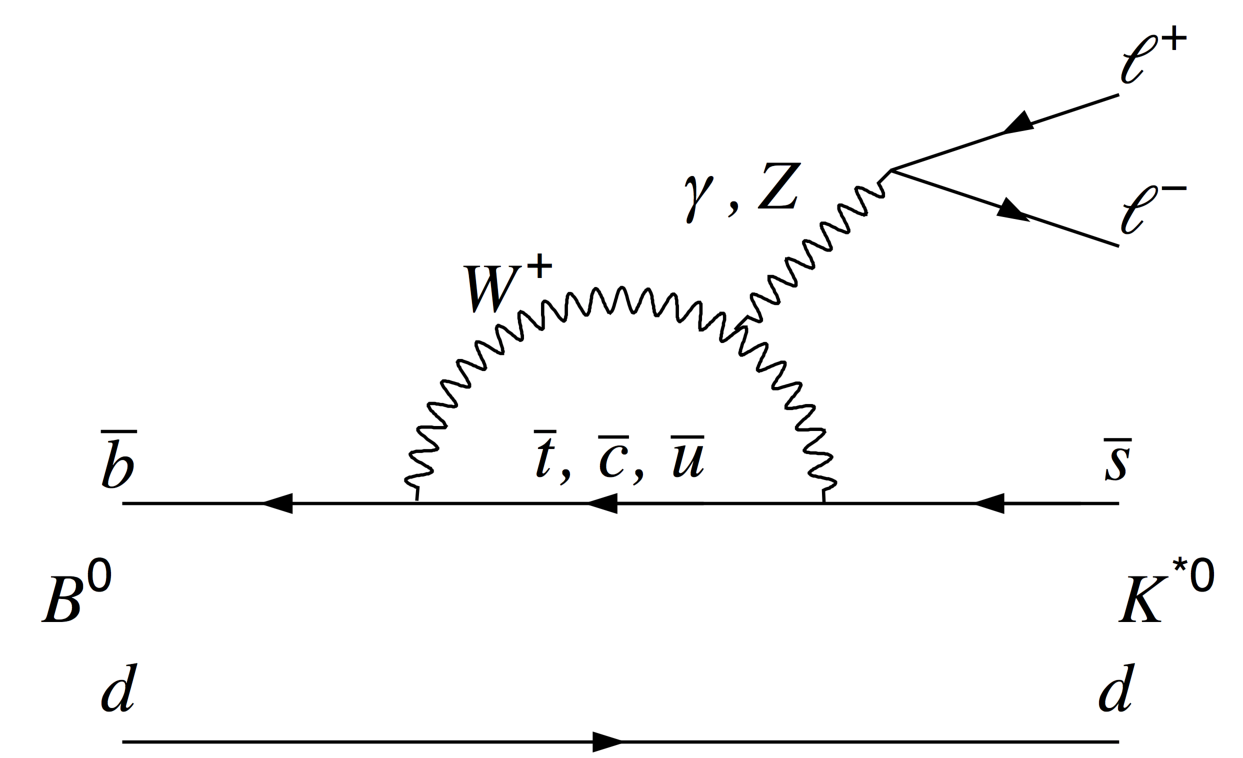
\includegraphics[width=0.57\linewidth]{figs/Fig1a.png}
  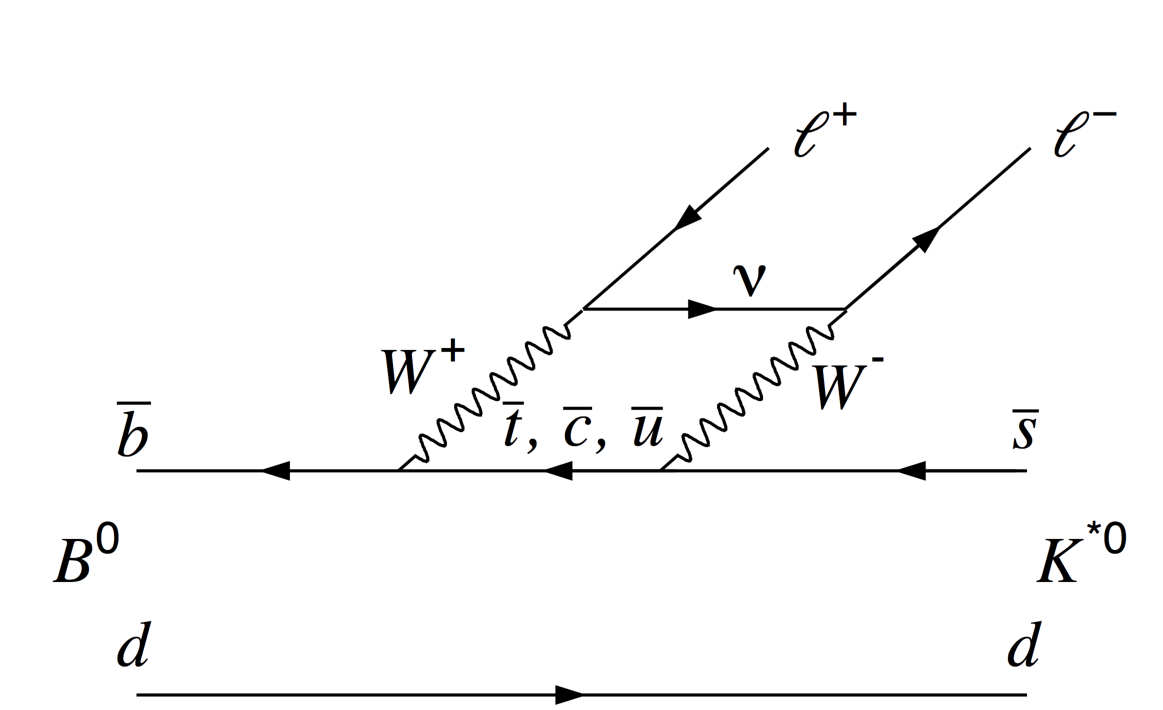
\includegraphics[width=0.57\linewidth]{figs/Fig1b.png}
\end{figure}
\begin{figure}[h!]
	\caption{If the Lepton universality is not satisfied (R(K$^{*}$,D$^{*} \neq$ 1), it implies there is new physics hidden in the diagram. It could be interpreted in terms of Lepto-quark or Electroweak Z boson which couples to right-hand chrial leptons.\cite{Lep:2017aai}}
  \label{fig:LU2}
  \centering
  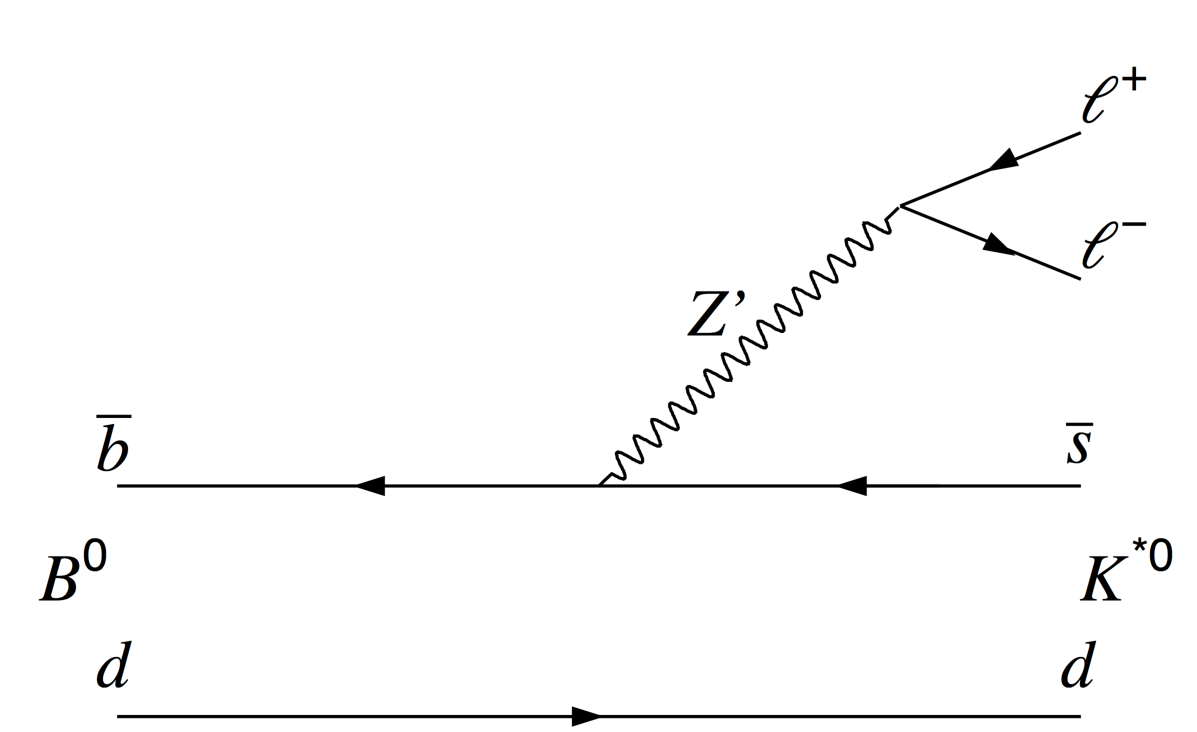
\includegraphics[width=0.57\linewidth]{figs/Fig1c.png}
  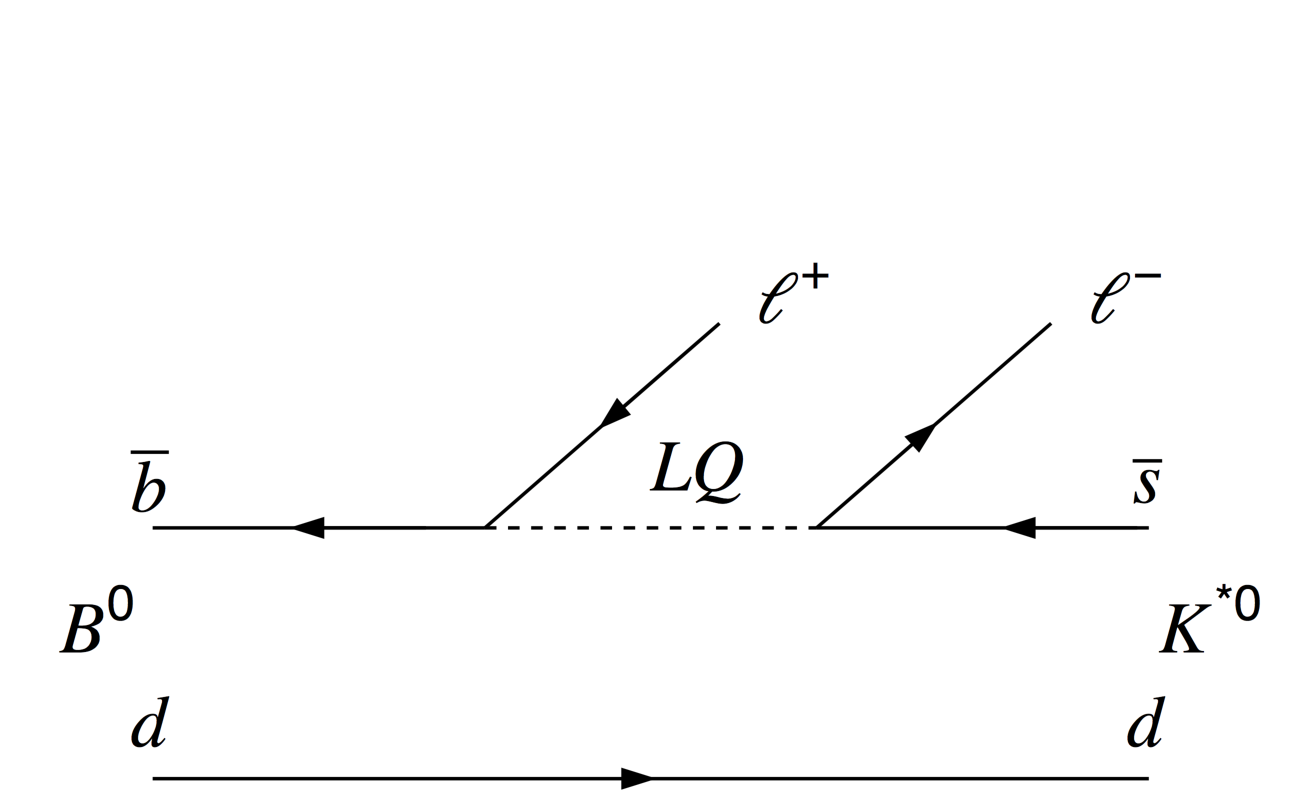
\includegraphics[width=0.57\linewidth]{figs/Fig1d.png}
\end{figure}
Because of this physics reason, the muon final state of B mesons are desired for research of R(K$^{*}$, D$^{*}$).
Consequently, the B-parking trigger requires a soft muon with modest displacement (measured using impact parameter) from the primary vertex, as in b-tagging.
It requires a muon with transverse momentum (pT) of 7-12 GeV with impact parameter (IP) significance 3-6.

Pp collisions in LHC produce enormous events, which could trigger the B parking trigger paths.
 As discussed in chapter \ref{sec:detectors}, the Current CPU capacity of CMS is limited and not capable of reconstructing the entire event at such a high trigger rate at the HLT level.
Thus, CMS scouts events, meaning it writes events that passed L1 trigger to a temporary dataset. 
Later, full HLT and RECO steps are implemented and serve as a B-Parking dataset.
The prescale factor for BPH triggers is 5-6.

\section{Trigger Paths}
We use data collected by the B-Parking triggers for the year of 2018.
The exact names of paths for B-Parking triggers are listed in Table~\ref{tab:triggers18}.
To compare with these data obtained from CMS detector, we get the Monte Carlo (MC) datasets for simulation of signal and background events.
Monte Carlo methods are computational algorithms to obtain physics results with statistical randomness.
CMS group uses this statistical instrument to publish various signal and background physics process MC datasets.
Using the generated signal MC, We plotted distributions of the generator level LLP's physics variables.
One can gauge triggering muons' IP significance values, pt, and isolation information.
\begin{table}[htb]
\caption{HLT trigger paths used in the analysis}
\begin{center}
\begin{tabular}{r|l}\hline
\hline
 Data sample & Trigger \\
\hline
 ParkingBPH*-Run2018A & HLT\_Mu9\_IP6\_part* \\
 ParkingBPH*-Run2018B & HLT\_Mu9\_IP6\_part* \\
 \hline
 ParkingBPH*-Run2018C & HLT\_Mu12\_IP6\_part* \\
 ParkingBPH*-Run2018D & HLT\_Mu12\_IP6\_part* \\
 \hline
 \hline
\end{tabular}
\label{tab:triggers18}
\end{center}
\end{table}

\begin{table}[htb]
\caption{Data and MC Global tags used for 2018 datasets}
\begin{center}
\begin{tabular}{r|l}\hline
 Data 2018 & 106X\_dataRun2\_v29 \\
 \hline
 MC 2018   & 106X\_upgrade2018\_realistic\_v11\_L1v1 \\
 \hline
\end{tabular}
\label{tab:GT}
\end{center}
\end{table}



\begin{figure}[h!]
  \caption{pt of the scalar products}
  \label{fig:scalarpt}
  \centering
  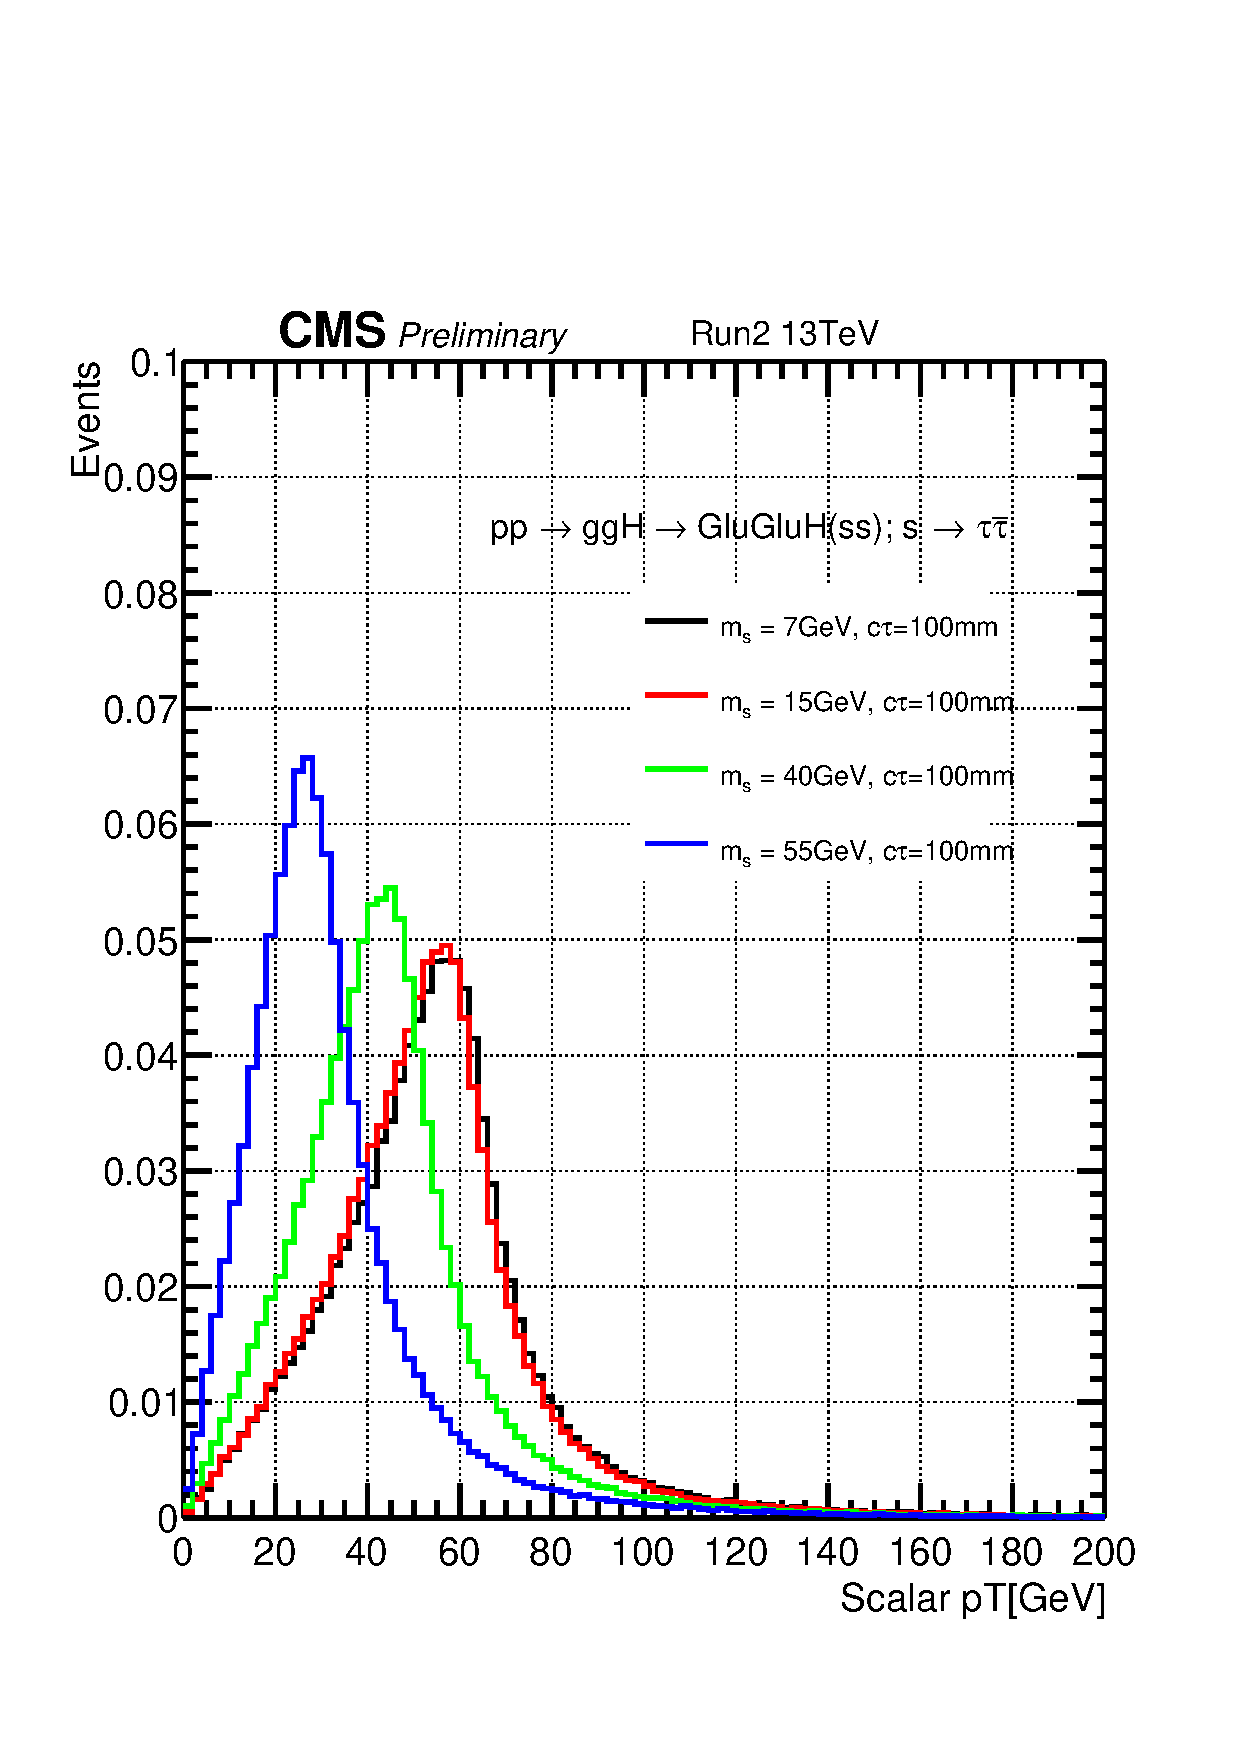
\includegraphics[width=0.5\linewidth]{figs/Scalar_pT100mm.pdf}
\end{figure}

\begin{figure}[h!]
  \caption{DeltaR of the scalar products}
  \label{fig:scalarpt}
  \centering
  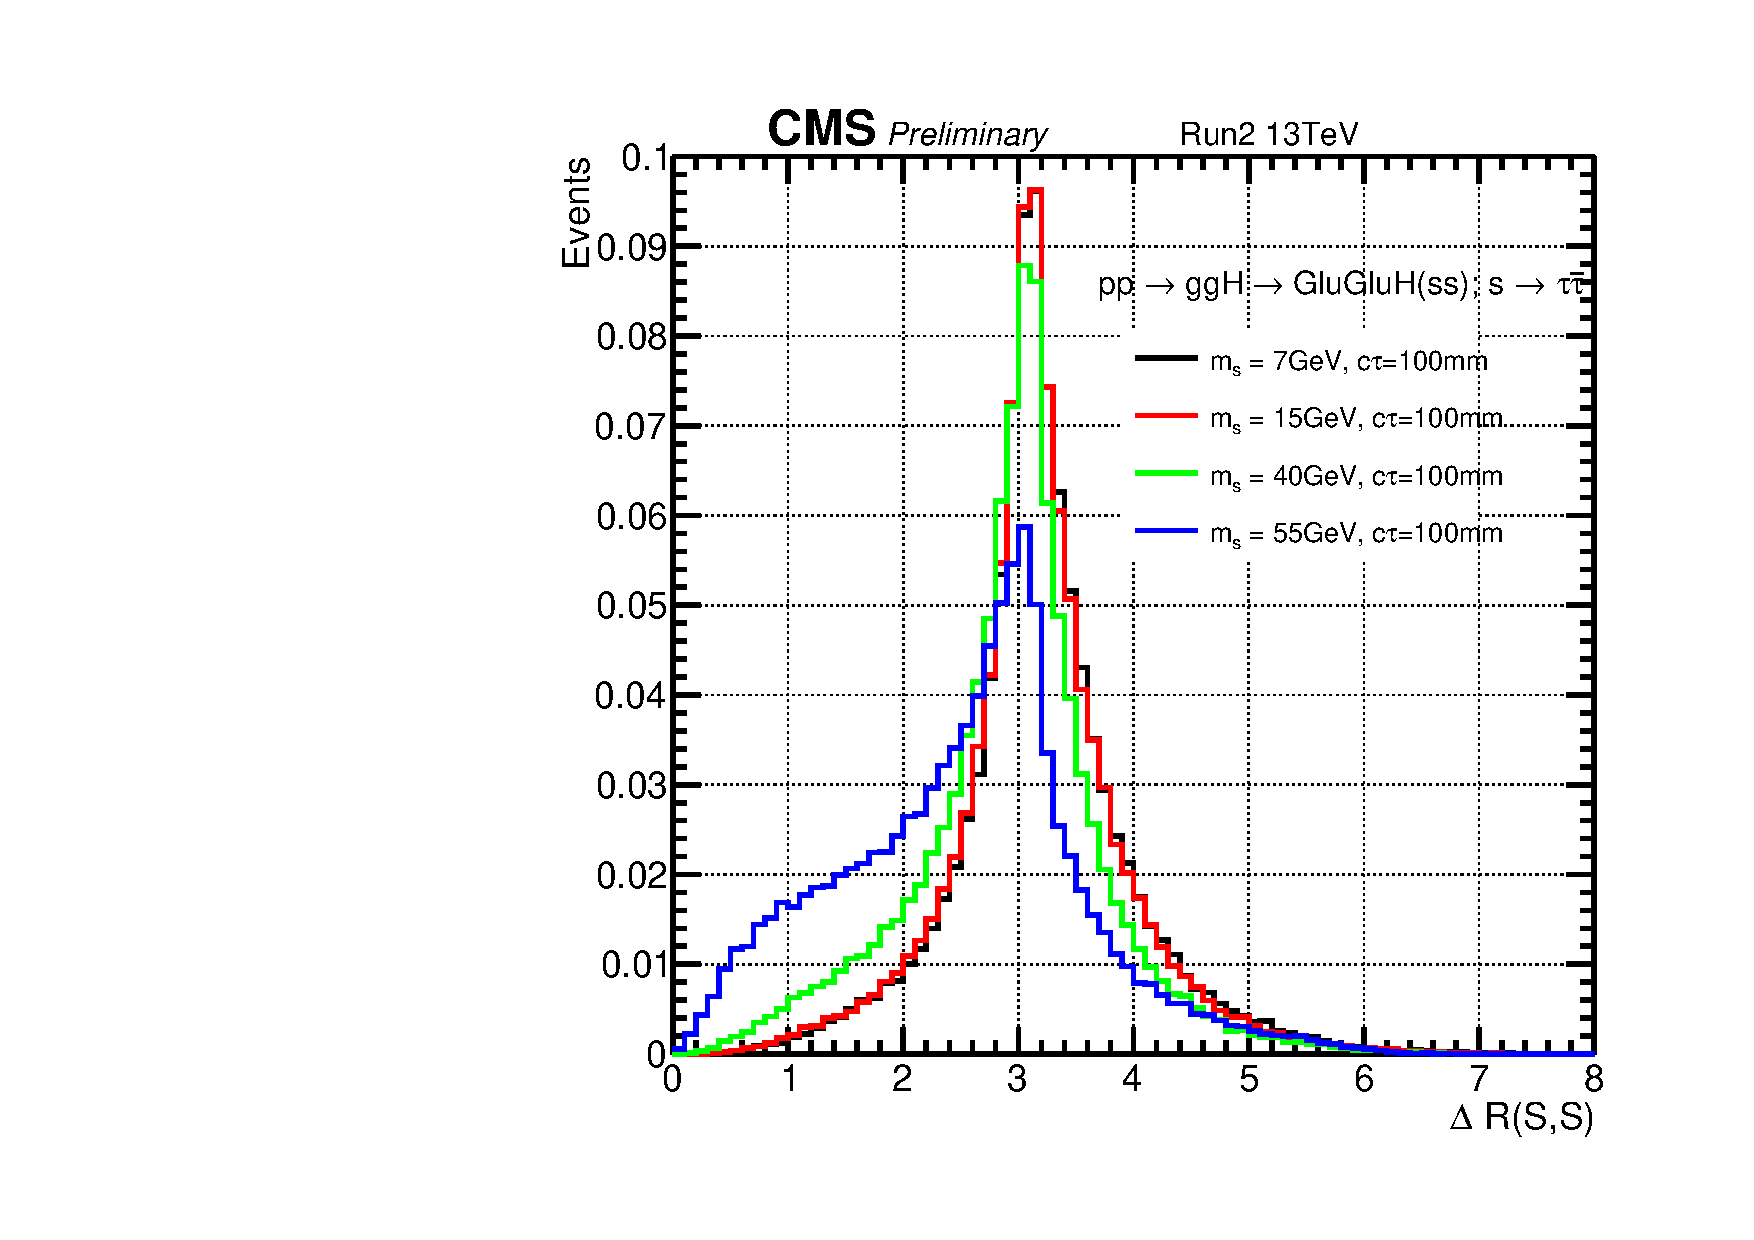
\includegraphics[width=0.5\linewidth]{figs/Scalar_dR100mm.pdf}
\end{figure}

\begin{figure}[h!]
  \caption{liftime of the scalar products in the lab frame}
  \label{fig:scalarpt}
  \centering
  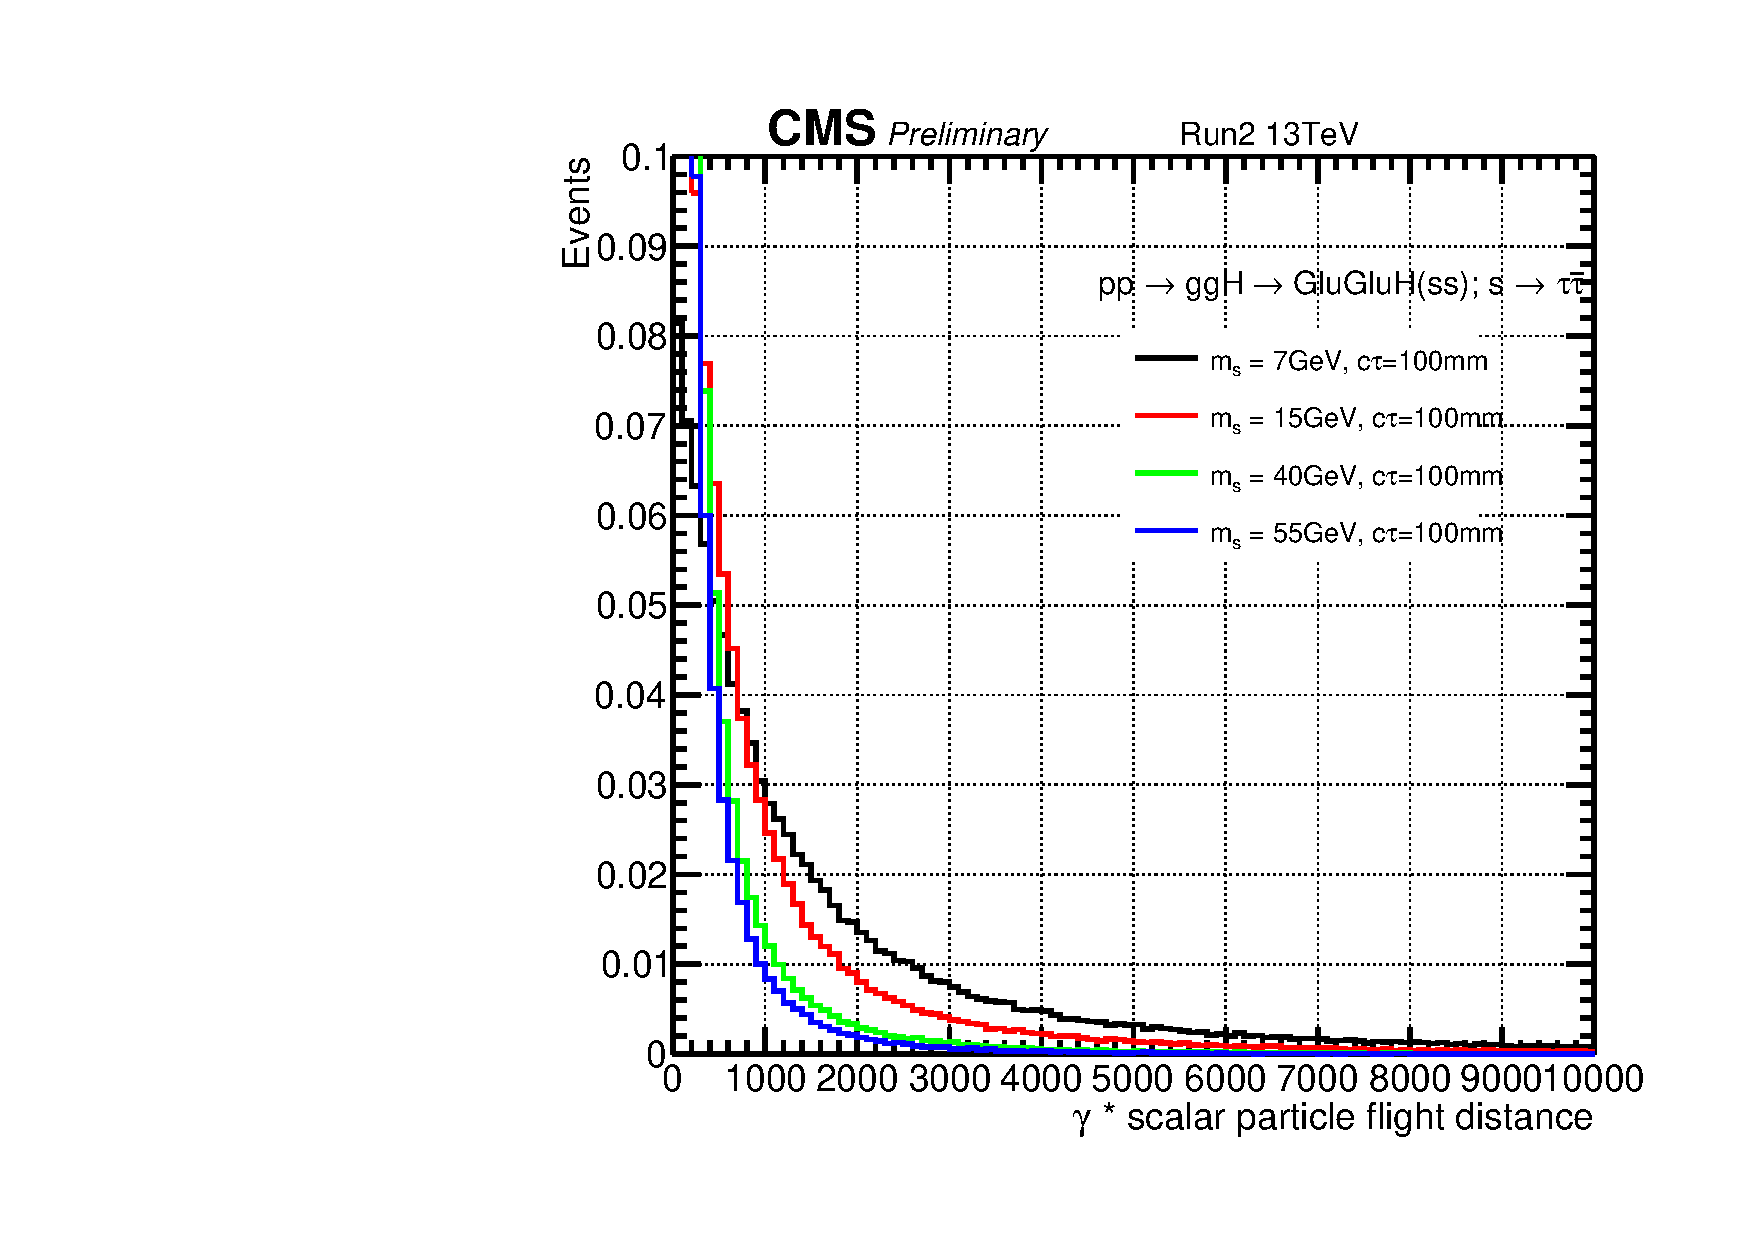
\includegraphics[width=0.57\linewidth]{figs/Scalar_gammactau100mm.pdf}
  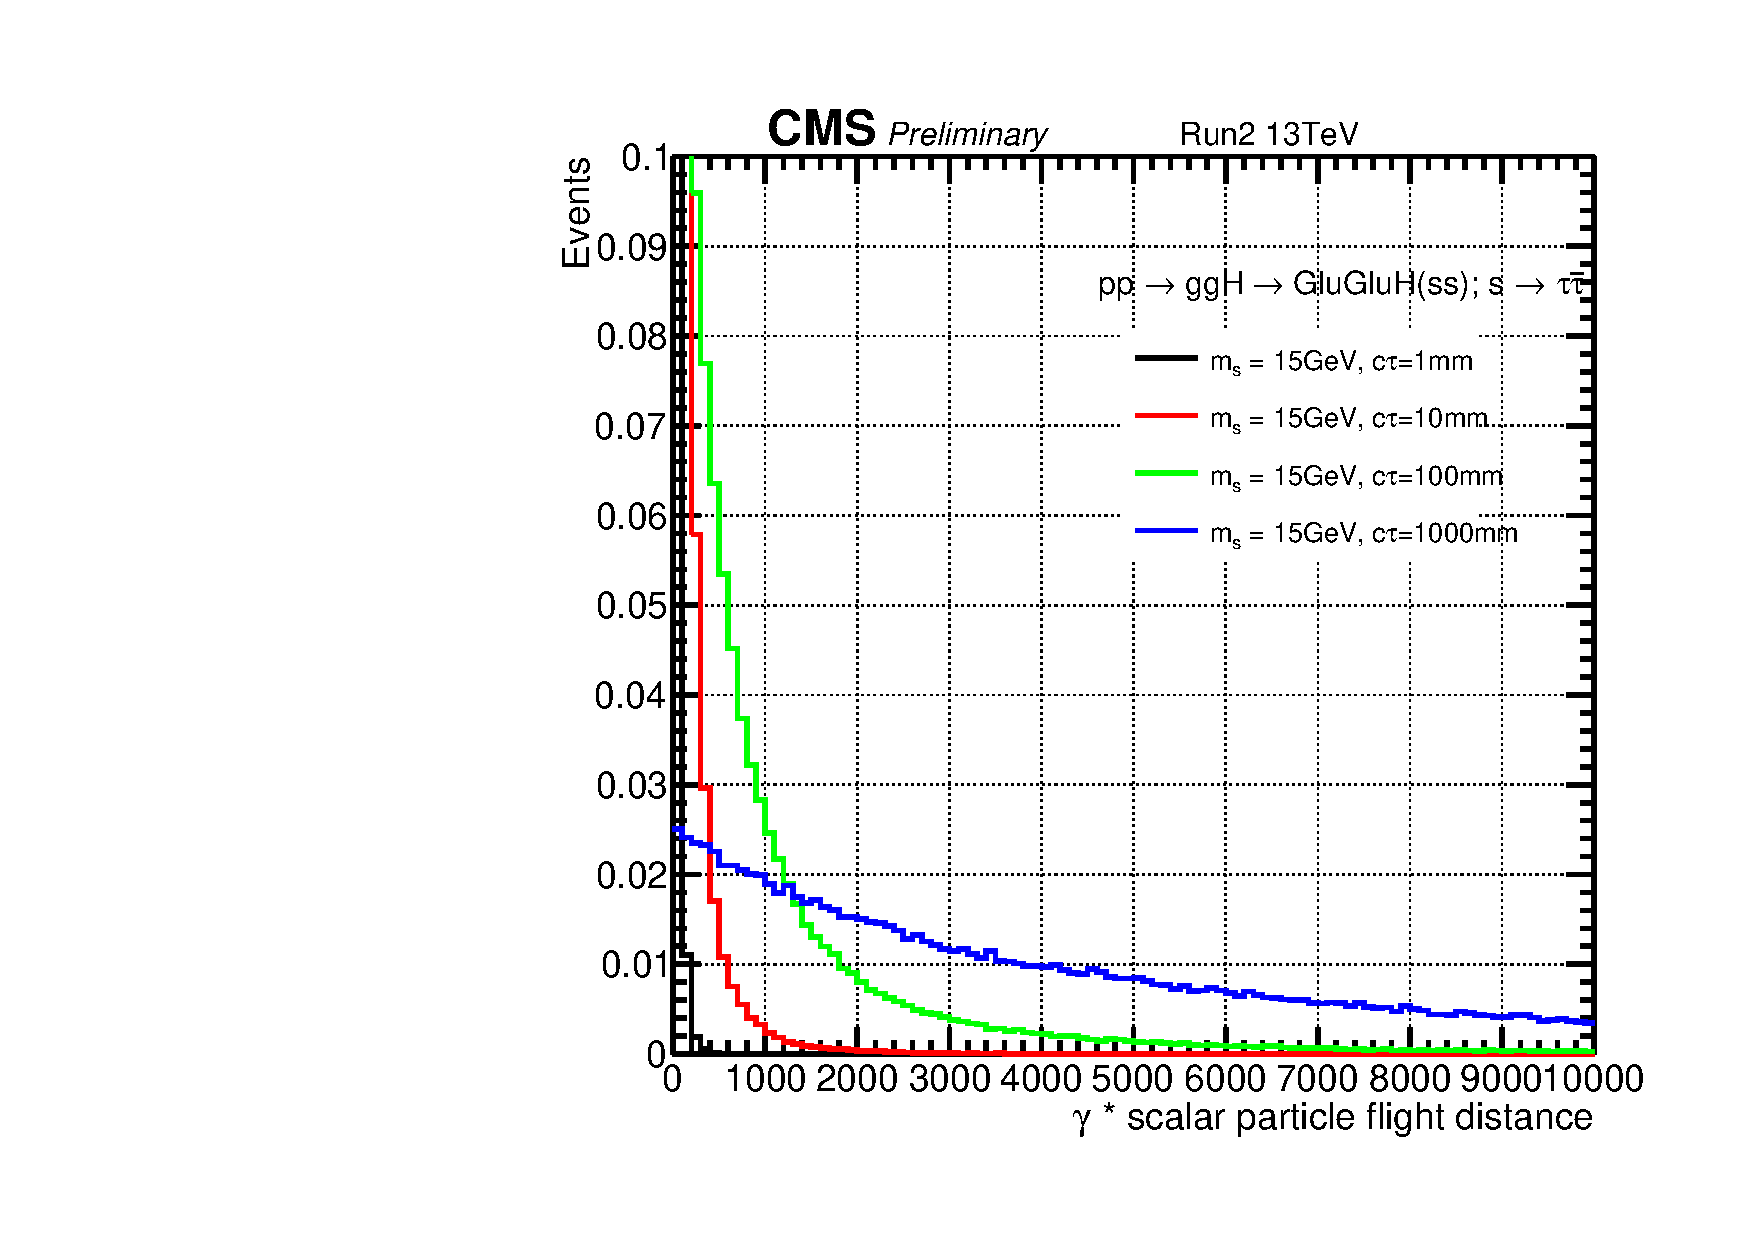
\includegraphics[width=0.57\linewidth]{figs/Scalar_gammactau15GeV.pdf}
\end{figure}

Below is the trigger efficiency of various BPH trigger paths for different mass scale and lifetime points of the signal ($H \to SS \to \tau\tau\tau\tau$) sample
The signal process shows an overall good efficiency.
Signal points with LLP's c$\tau$ = 10,100mm show the best performance.
Signal points with LLP's c$\tau$ = 1000mm likely decay outside of the tracker region, leaving no track's impact parameter, and fails to pass the trigger.
On the other hand signal point with LLP's c$\tau$ = 1mm may not reach the first-pixel detector, which is at 2.7cm from the beam spot, and fails to pass the trigger.
We can confirm this explanation by observing that lighter LLP has better trigger efficiency for a shorter lifetime thanks to a more significant boost and vice versa for heavier LLP.
\begin{figure}[h!]
	\caption{The plots show the trigger efficiency for each HLT path with respect to LLP's lifetime. Each line denotes mass scale of each LLP. Please note the efficiency is set to 0 for MS=7GeV c$\tau$ = 1mm due to absece of Monte Carlo (MC).}
  \label{fig:Trigger Efficiency}
  \centering
  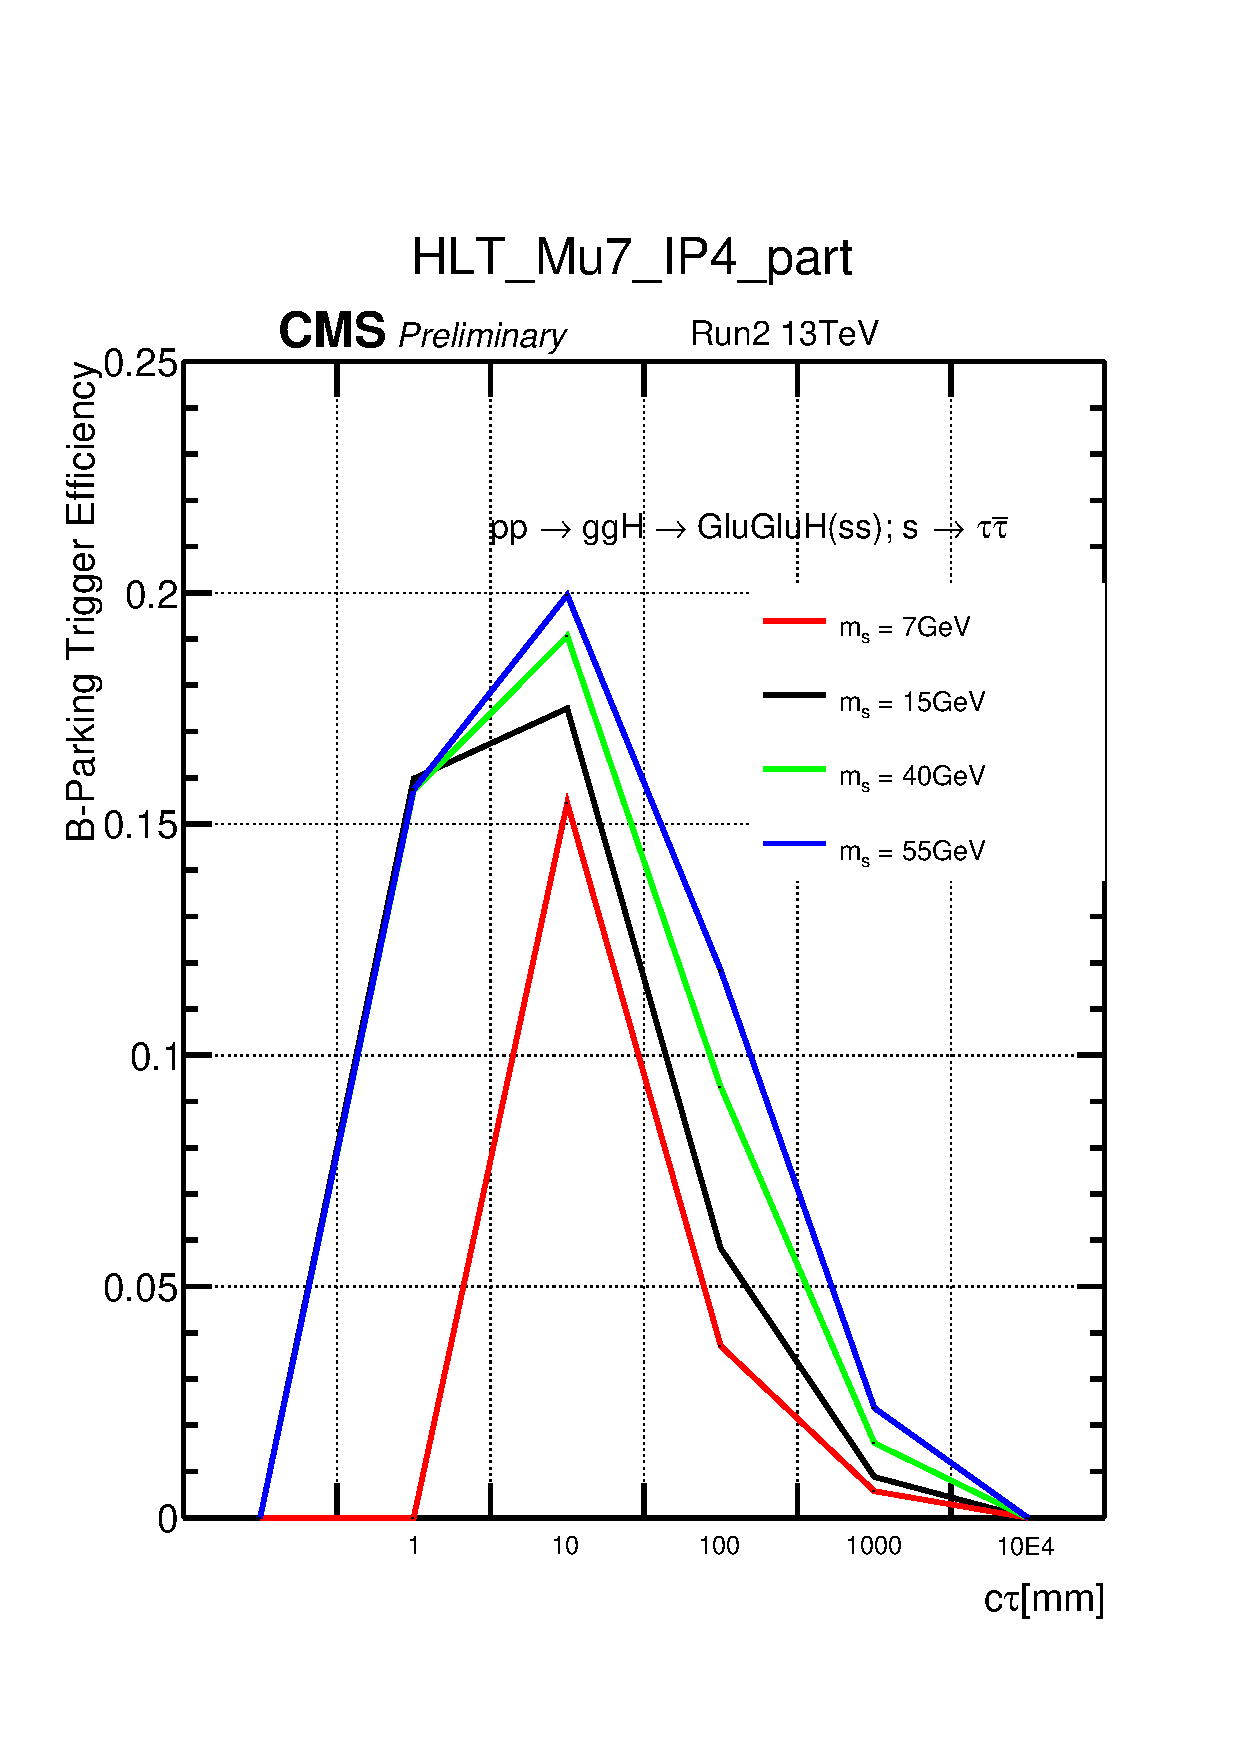
\includegraphics[width=0.47\linewidth]{figs/TrigEff_HLT_Mu7_IP4_part.pdf}
  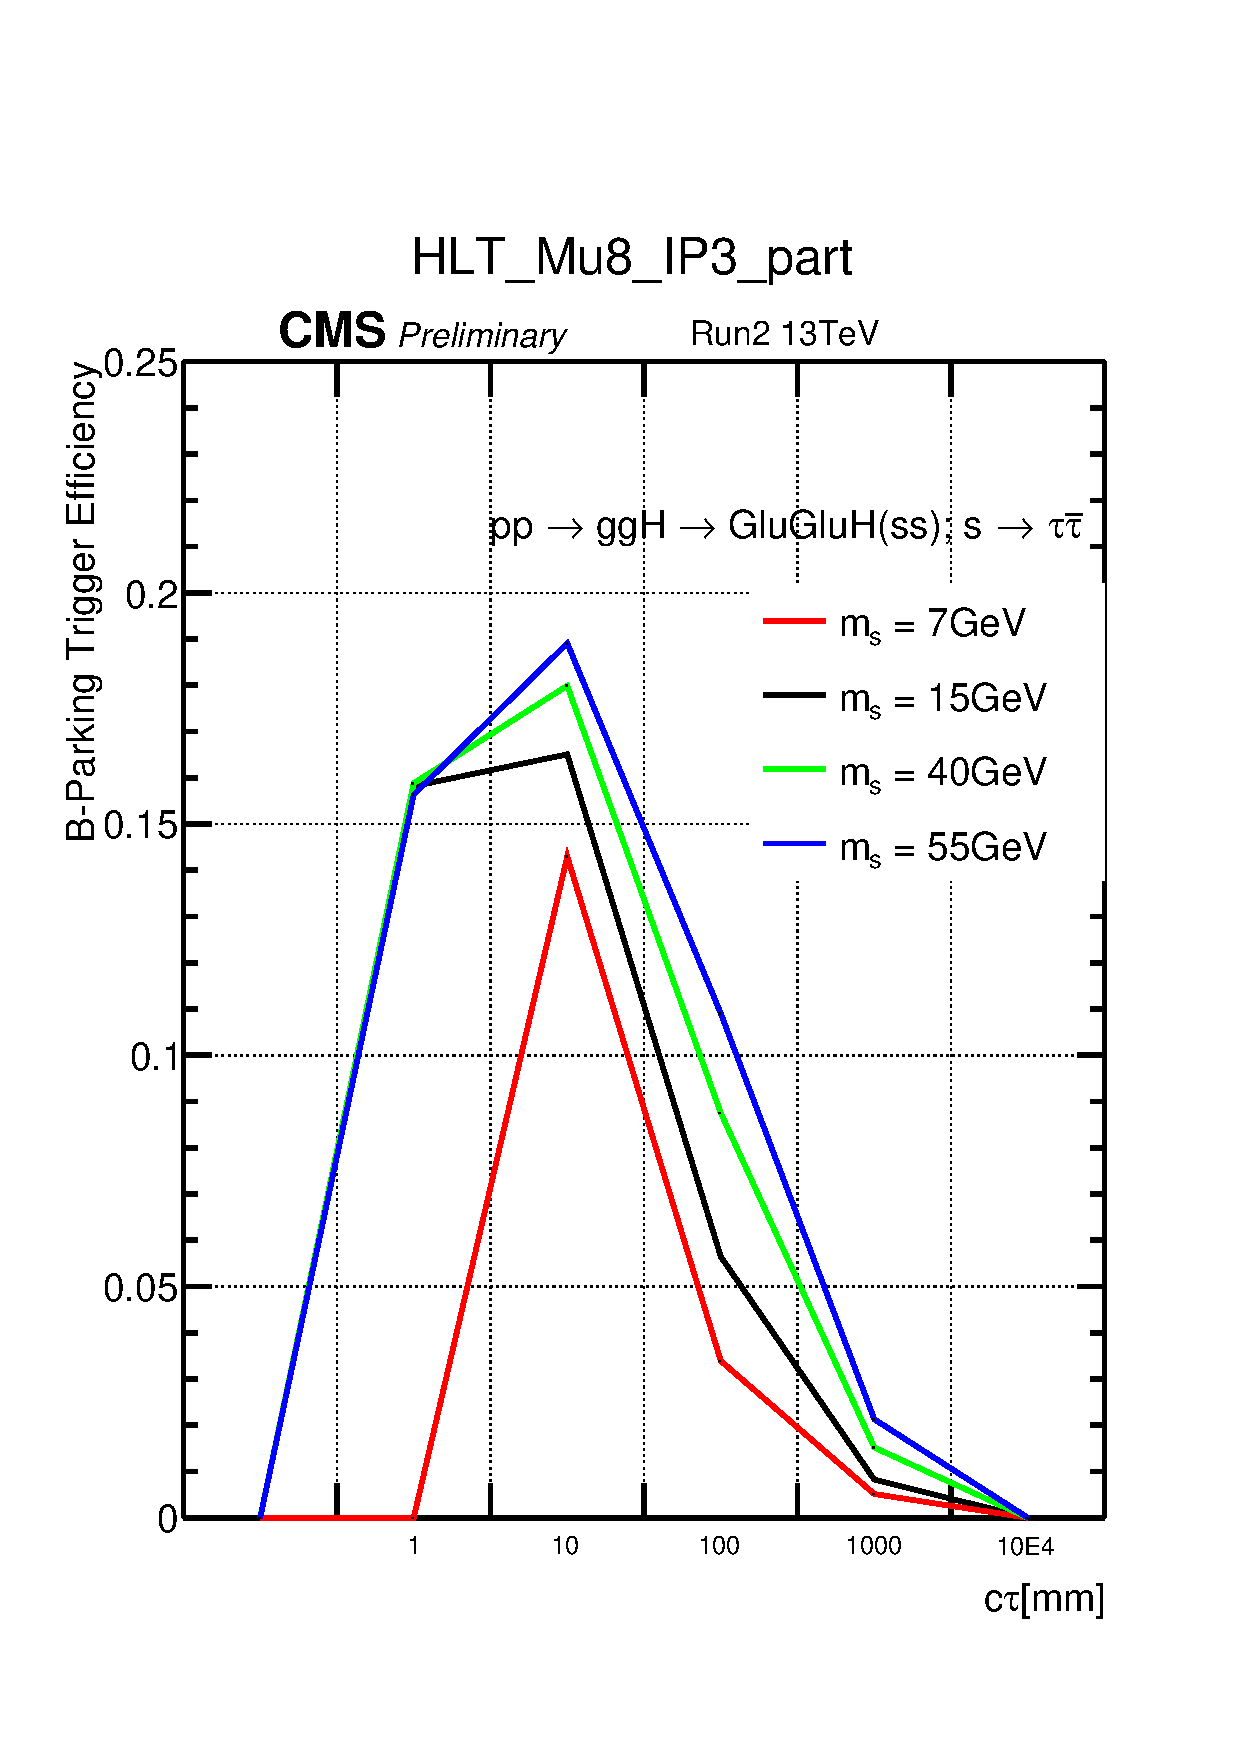
\includegraphics[width=0.47\linewidth]{figs/TrigEff_HLT_Mu8_IP3_part.pdf}

\end{figure}
\begin{figure}[h!]
\caption{The plots show the trigger efficiency for each HLT path with respect to LLP's lifetime. Each line denotes mass scale of each LLP. The analysis uses Mu9\_IP6 for Era A,B of data and Mu12\_IP6 for Era C,D of data. Please note the efficiency is set to 0 for MS=7GeV c$\tau$ = 1mm due to absece of Monte Carlo (MC).}
  \centering
  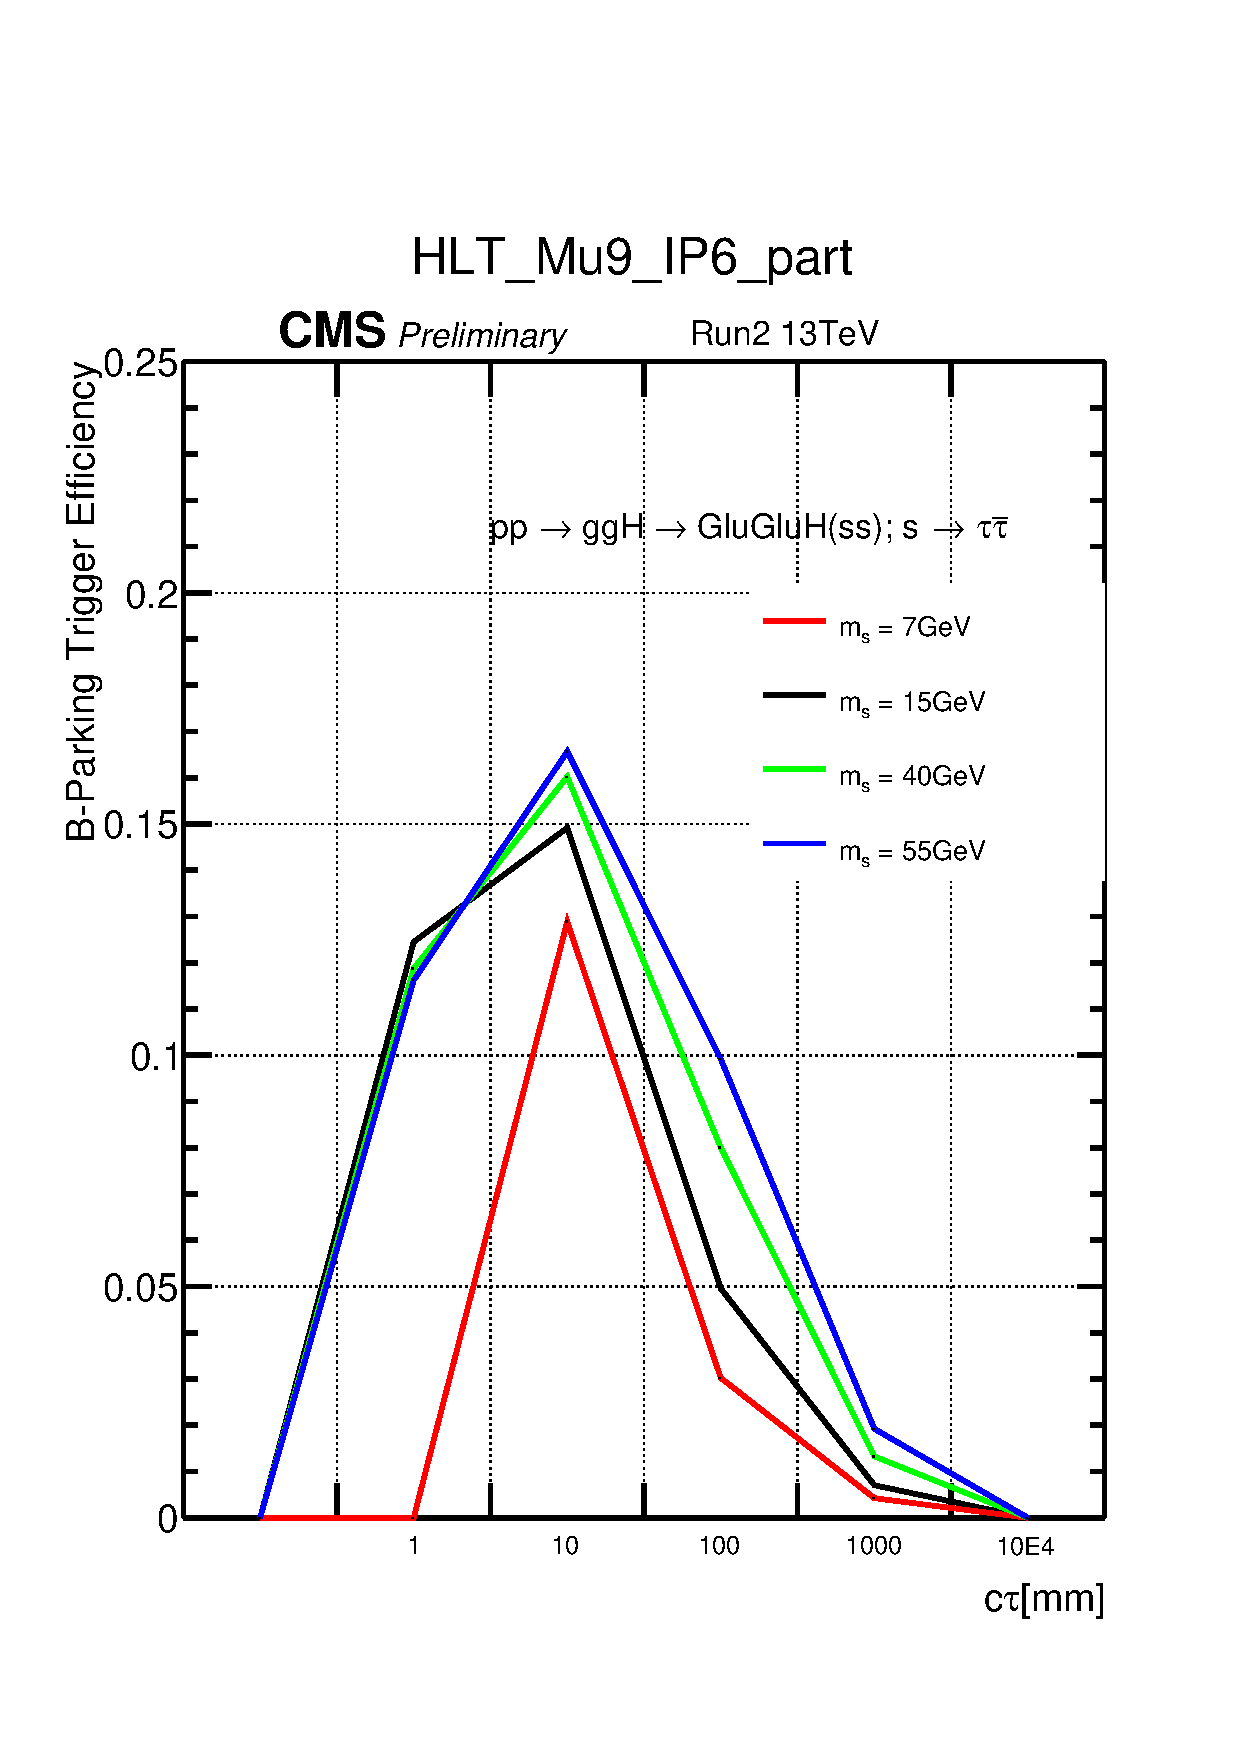
\includegraphics[width=0.47\linewidth]{figs/TrigEff_HLT_Mu9_IP6_part.pdf}
  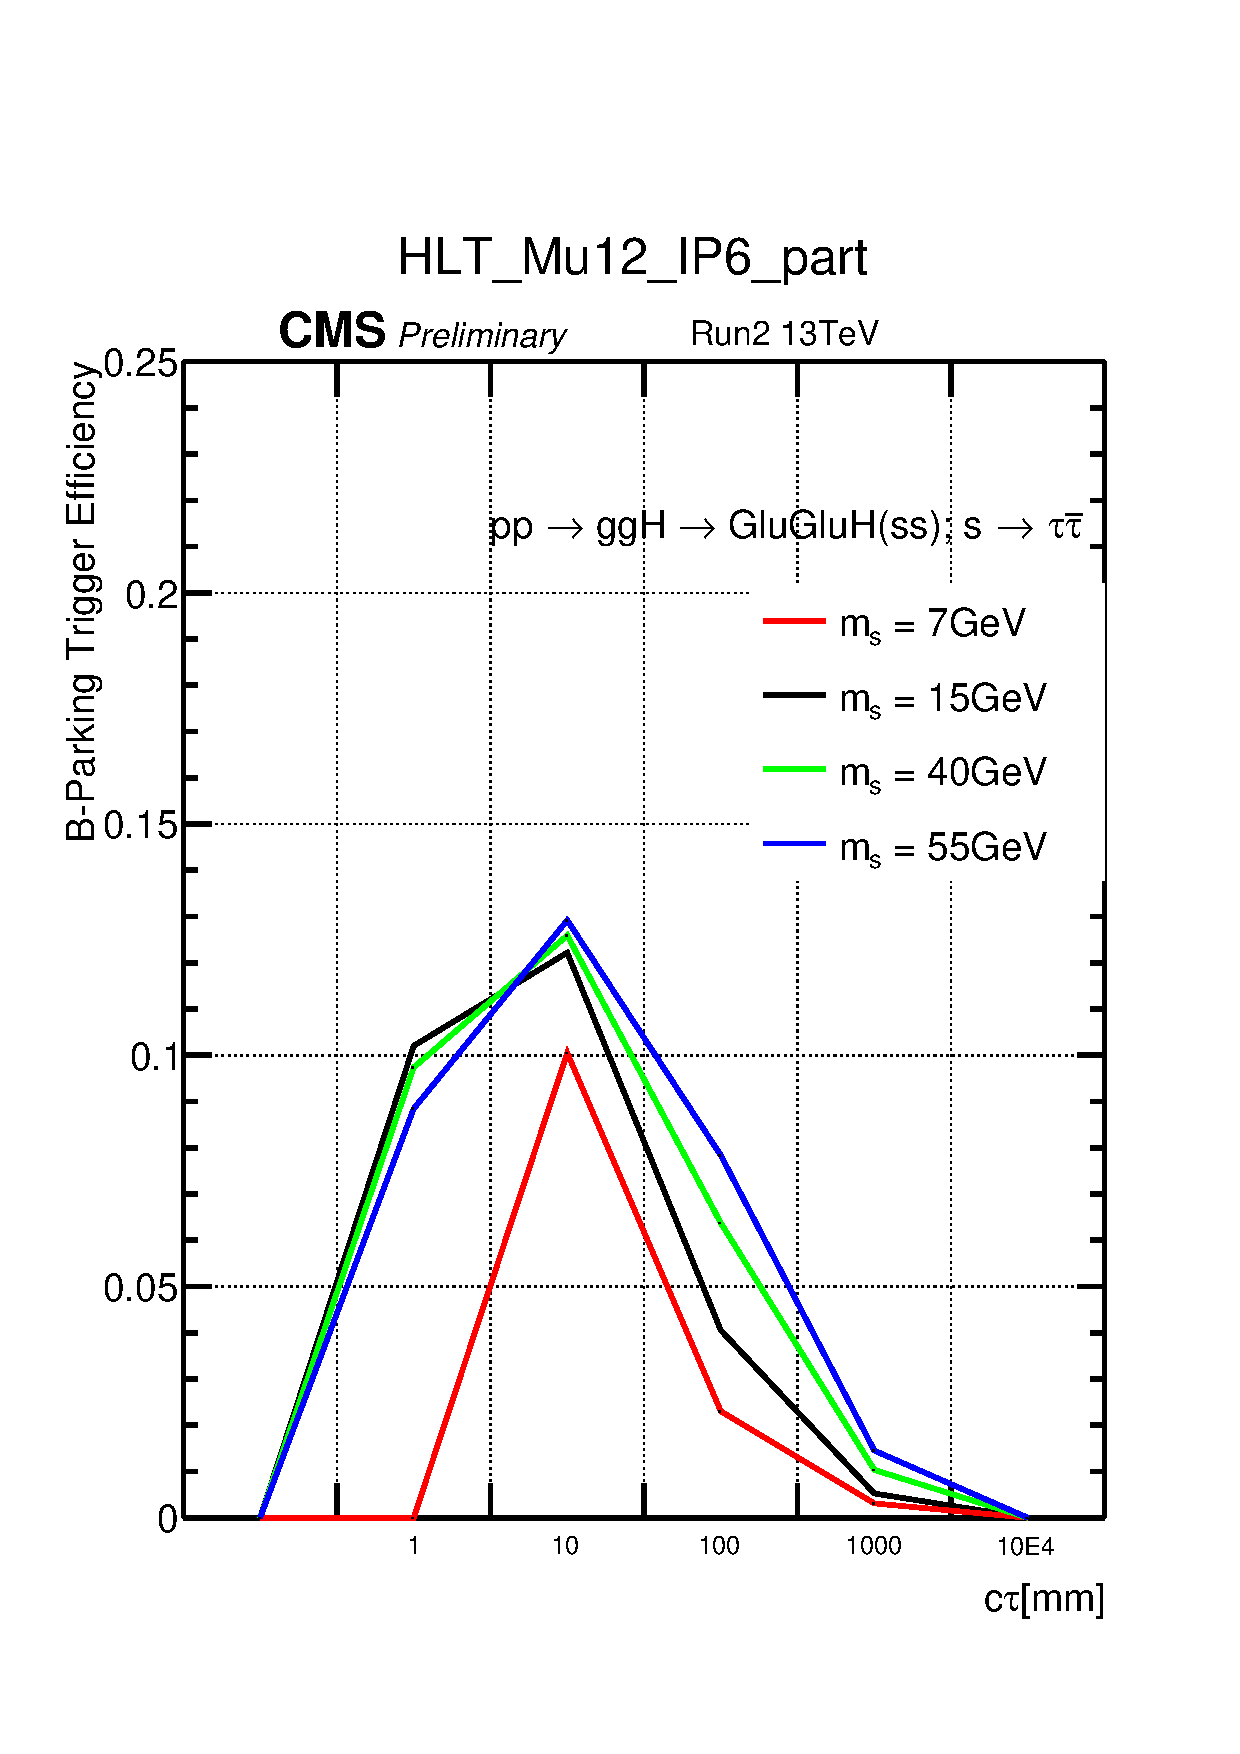
\includegraphics[width=0.47\linewidth]{figs/TrigEff_HLT_Mu12_IP6_part.pdf}

\end{figure}

In contrast to the signal, the background processes show poor trigger efficiency.
TTJets, Single Tops, and QCD pass the trigger at low but non-negligible efficiency.
All these background processes have heavy flavor particles for their final state (b-quark or top quark).
From the trigger efficiency and enormous cross-section of the QCD process, we can infer that the QCD process will become a significant contribution to our background.
Many physics analyses groups across CMS use the QCD MC datasets.
Thanks to their popularity and need for heavy statistics, CMS group generates QCD MC datasets filtered to different groups' focuses.
We use QCD's Muon Enriched datasets to improve background events' statistics, which would pass the B Parking trigger.
CMS group names the dataset QCD-MuEnrichedPt5, with QCD's muon decay product passing a pT threshold of 5 GeV.
QCD-MuEnriched has better efficiency for higher Pt bin samples since higher Pt bin samples tend to have more b-jets for their final state.
Drell-Yan and W-Jet processes show a very poor trigger efficiency due to the absence of heavy flavor particles in their final state.


\section{Integrated Luminosity and pileup weight for the HLT path}
The integrated luminosity for each era has been summarized in table \ref{tab:datasample2018BPH} in Appendix A.
The information was obtained with commands in section \ref{sec:PU} of Appendix A.
The integrated Luminosity totals at 44$fb^{-1}$ lower than 58.7$fb^{-1}$ for the year of 2018.
The bunch-crossing for the B-parking HLT path is also very different from other HLT paths.
As expected, b-parking data are recorded during lower bunch-crossing runs due to its extreme rate in CMS collider.

It is vital to adjust this bunch-crossing variable for MC simulation to model the data correctly.
To achieve this purpose, we apply pileup weight to the MC simulation.
Pileup weight is simply a bunch-crossing of data divided by the bunch-crossing of MC for a specific era.
Pileup (PU) weight values are calculated for each era of data-taking (A, B, C, D).
Figure~\ref{fig:EraAData} shows the BPH1-Era A's HLT\_Mu9\_IP6 HLT path's Data PU distribution.
\begin{figure}[h!]
  \caption{Bunch crossing of dataset /ParkingBPH1/Run2018A-UL2018\_MiniAODv2-v1/MINIAOD}
  \label{fig:EraAData}
  \centering
  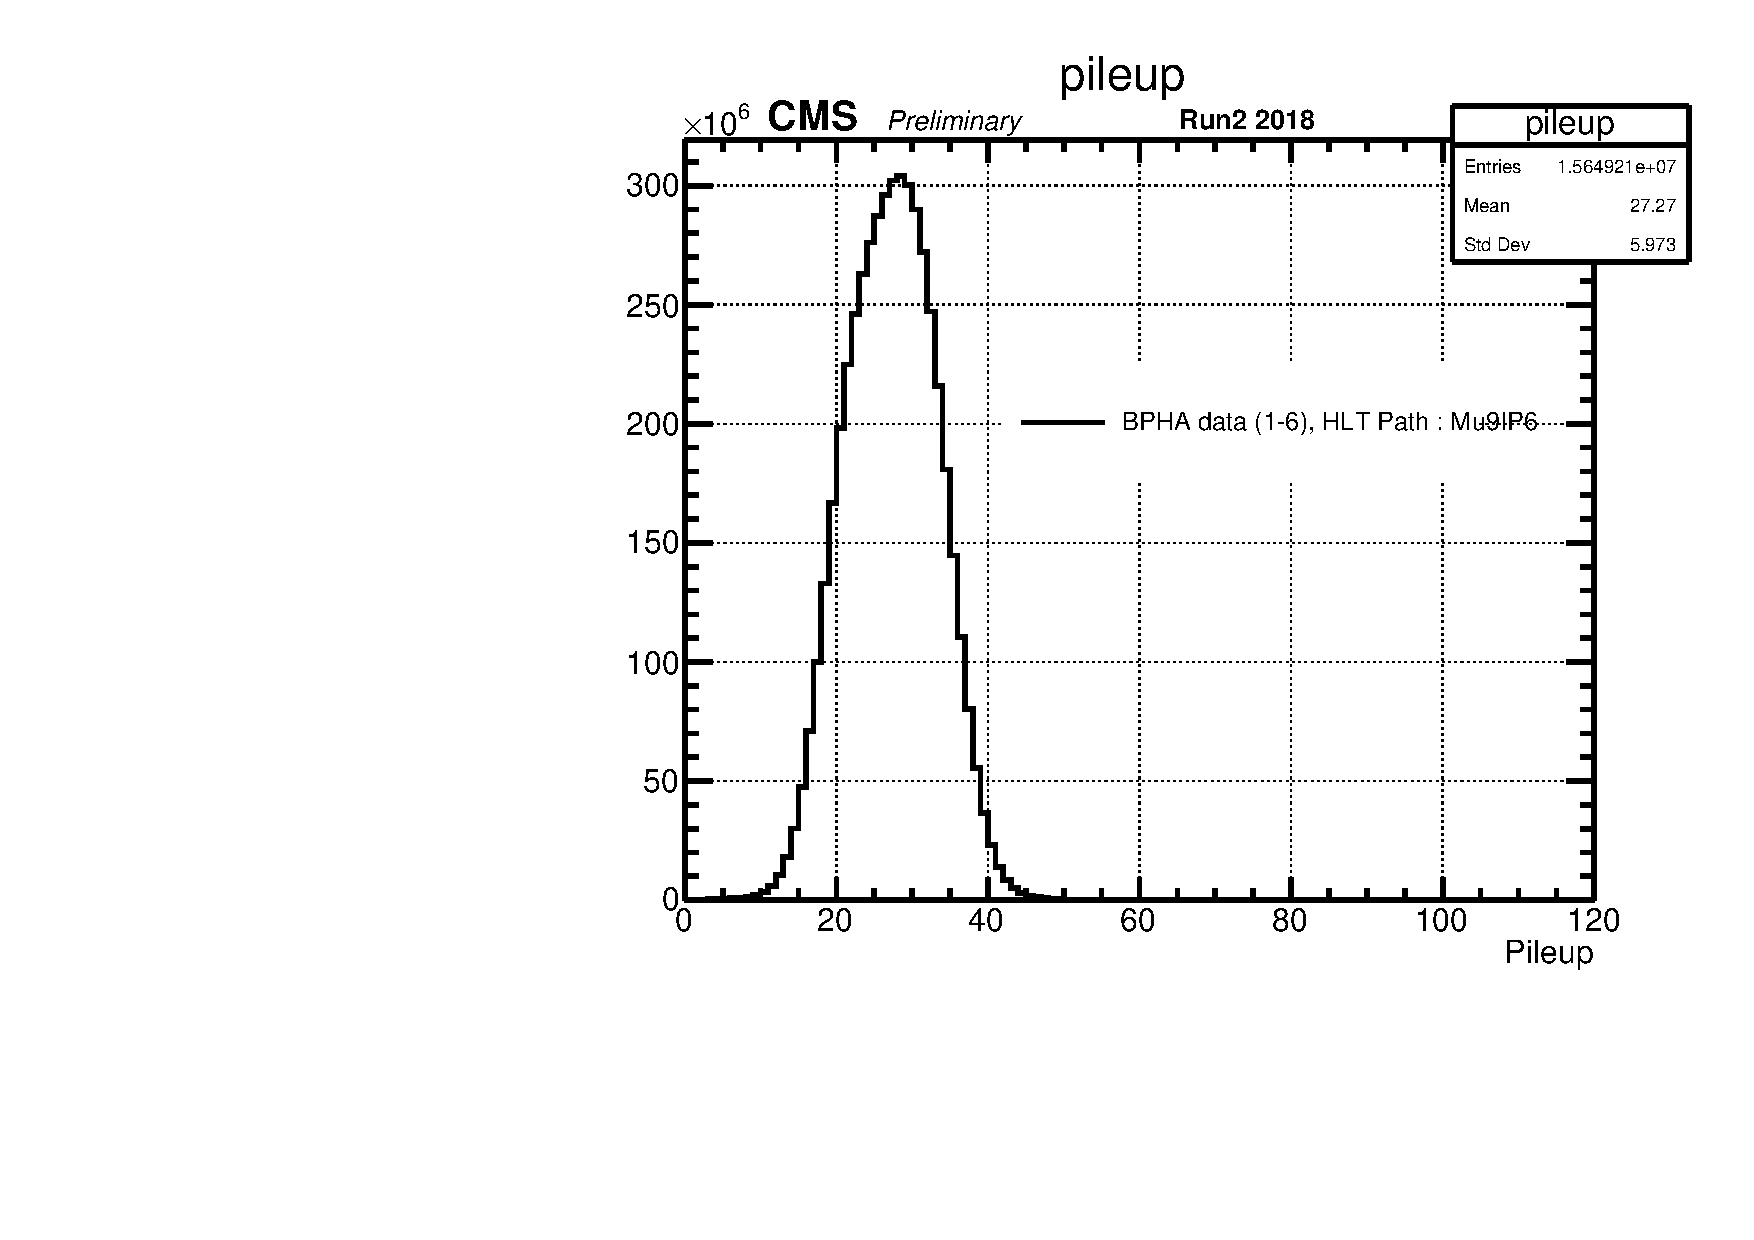
\includegraphics[width=0.67\linewidth]{figs/NVtx_BPHA.pdf}

\end{figure}

Figure~\ref{fig:EraAData} shows the BPH1-Era B's HLT\_Mu9\_IP6 HLT path's Data PU distribution.
\begin{figure}[h!]
  \caption{Bunch crossing of dataset /ParkingBPH1/Run2018B-UL2018\_MiniAODv2-v1/MINIAOD}
  \label{fig:EraAData}
  \centering
  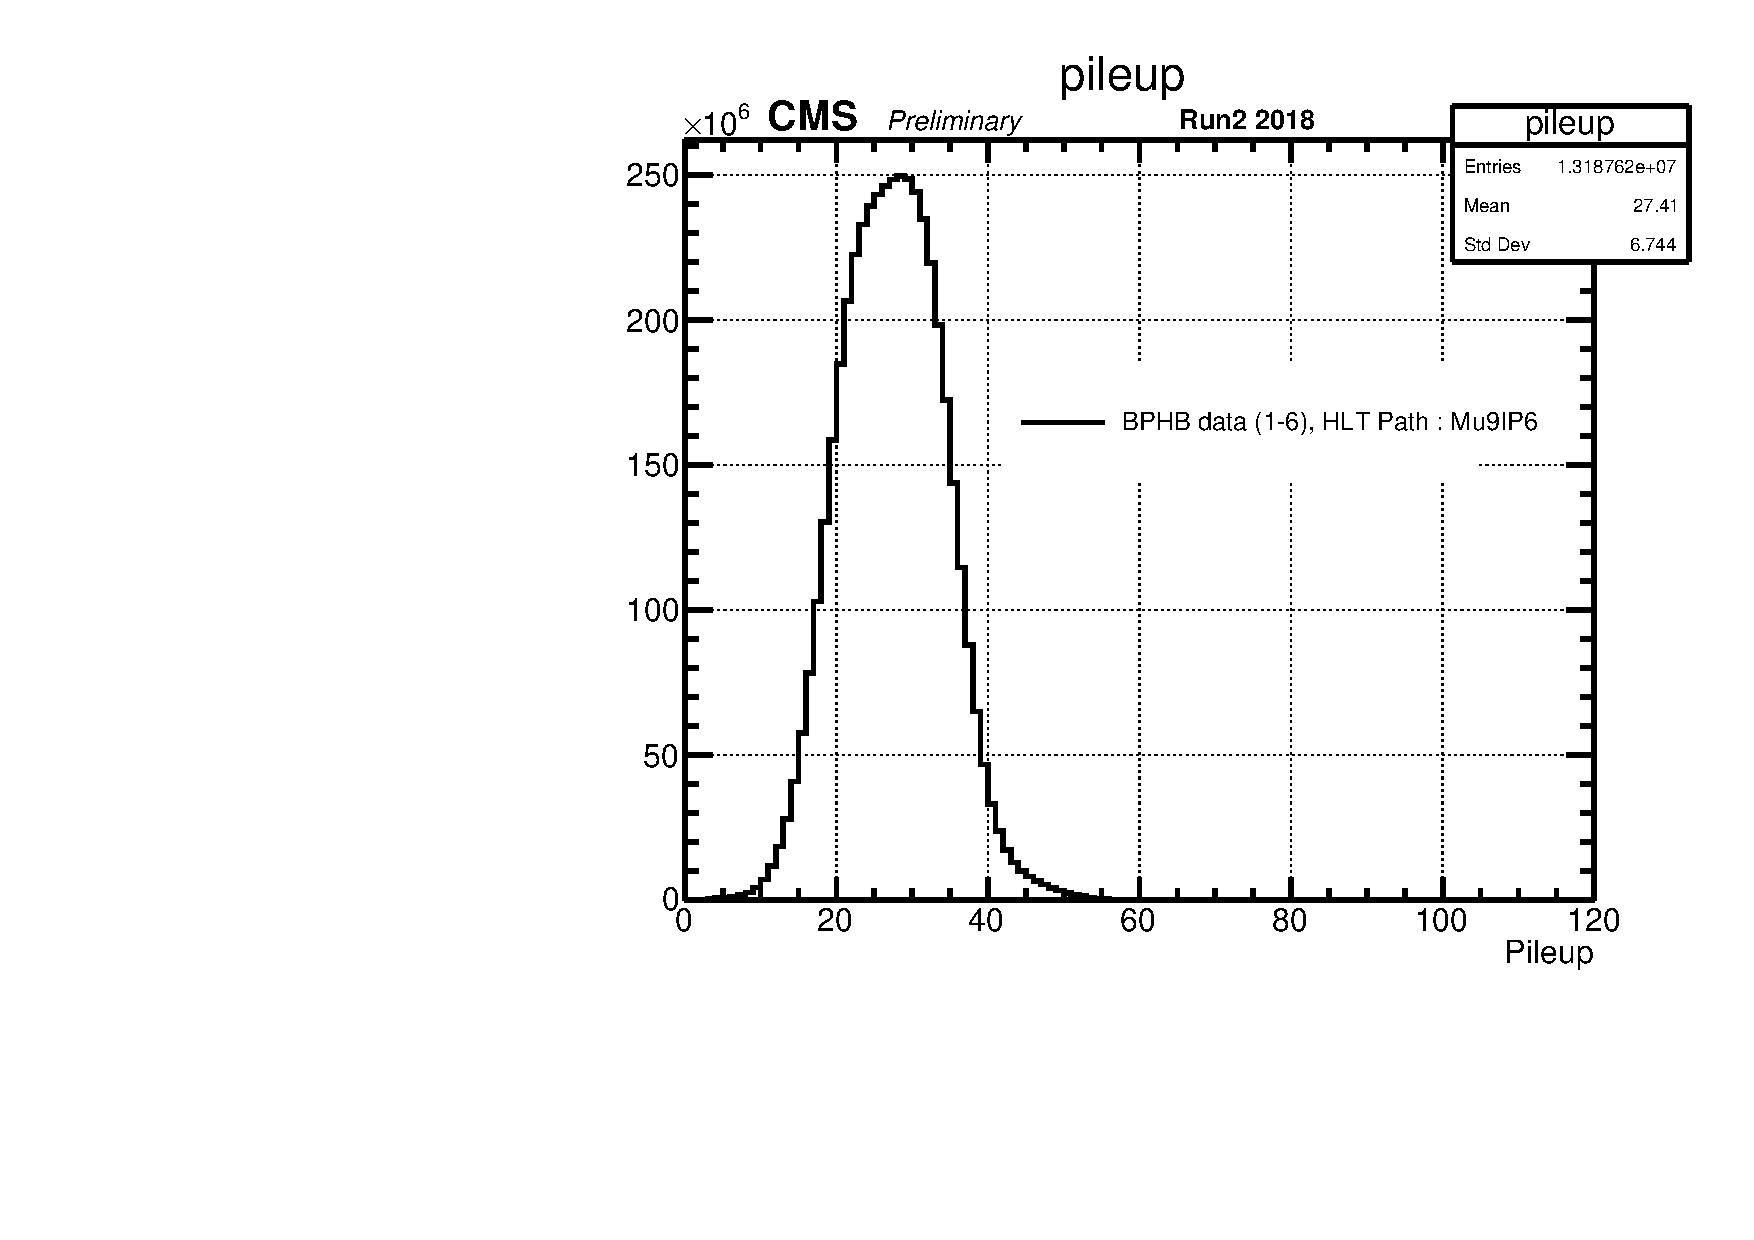
\includegraphics[width=0.67\linewidth]{figs/NVtx_BPHB.pdf}

\end{figure}

Figure~\ref{fig:EraCData} shows the BPH1-Era C's HLT\_Mu12\_IP6 HLT path's Data PU distribution.
\begin{figure}[h!]
\caption{Bunch crossing of dataset /ParkingBPH1/Run2018C-UL2018\_MiniAODv2-v1/MINIAOD. Please note that the HLT path for EraC has higher muon object's pT threshold with 12GeV (compared to 9GeV in EraA).}
  \label{fig:EraCData}
  \centering
  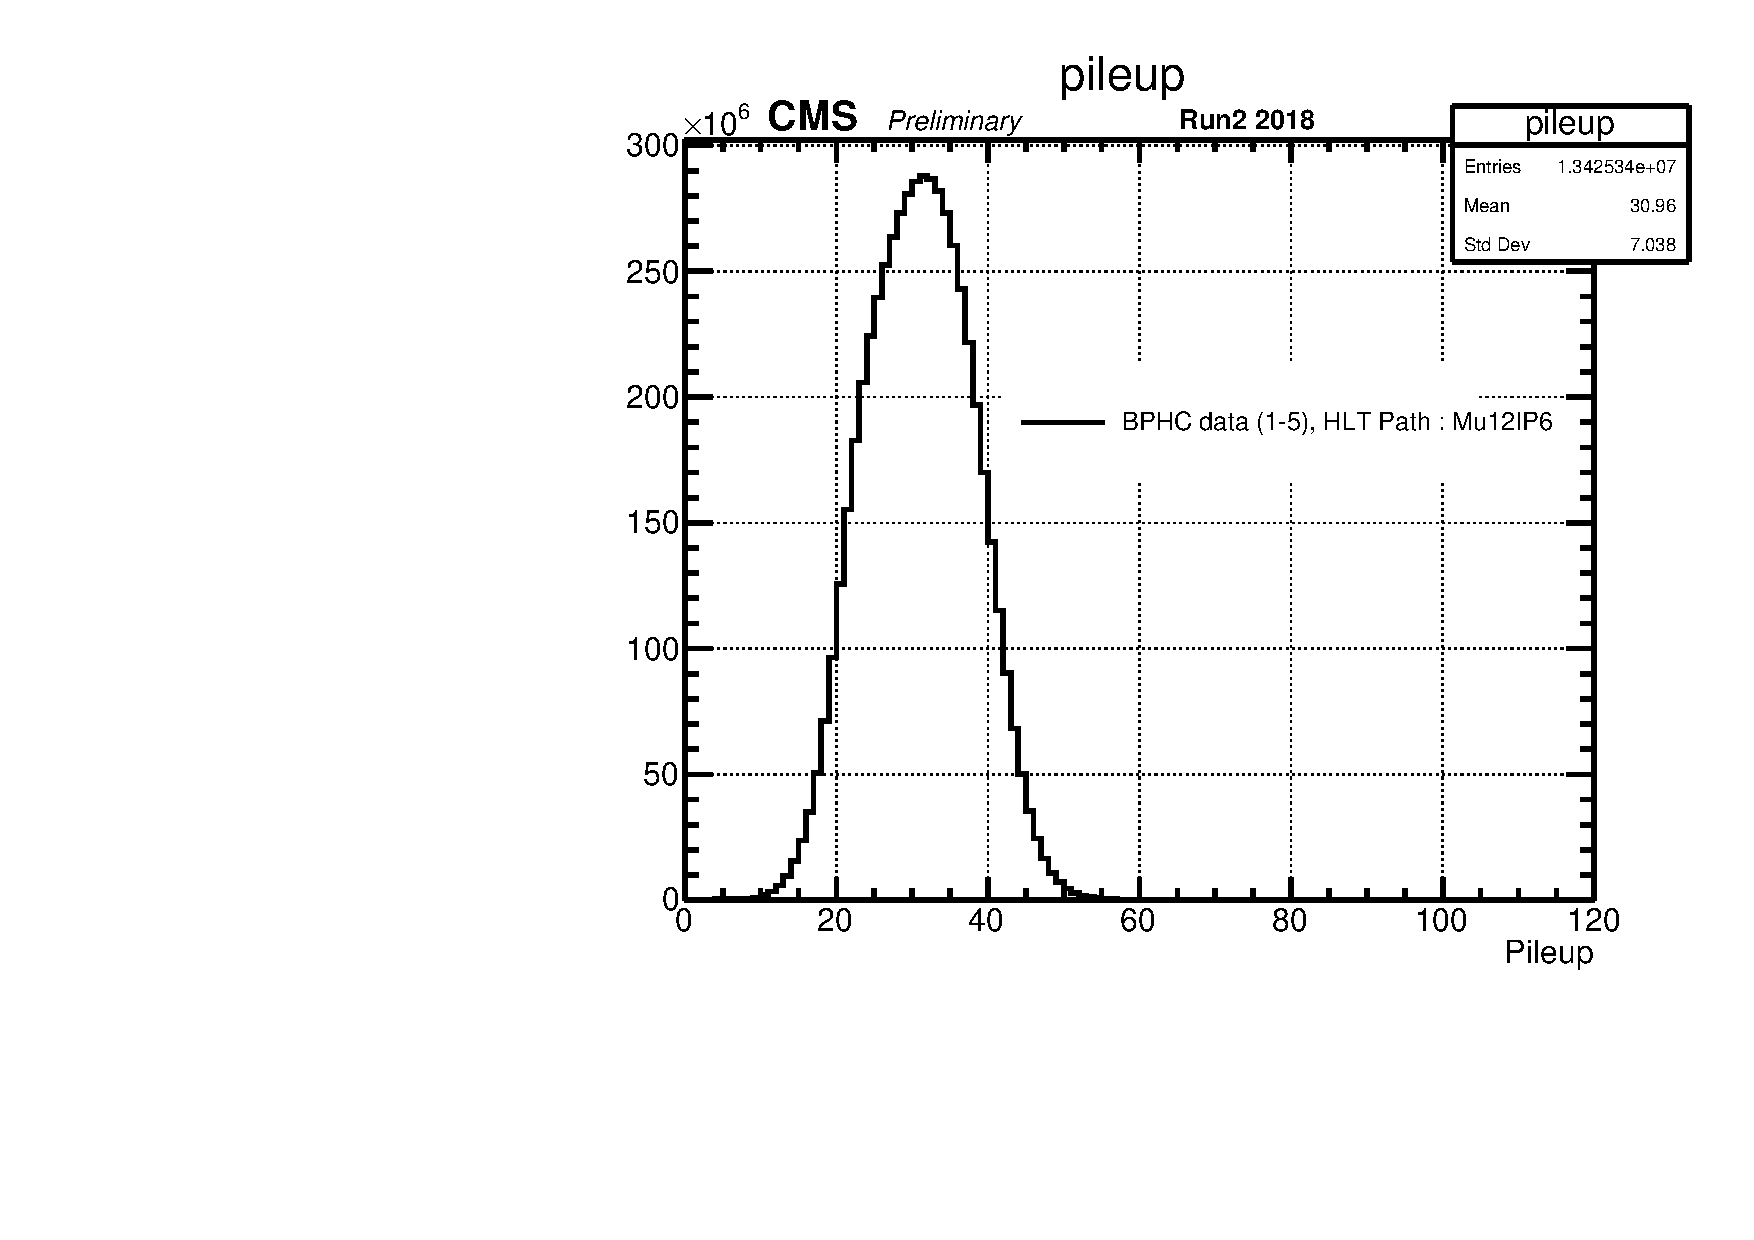
\includegraphics[width=0.57\linewidth]{figs/NVtx_BPHC.pdf}

\end{figure}

Figure~\ref{fig:EraCData} shows the BPH1-Era D's HLT\_Mu12\_IP6 HLT path's Data PU distribution.
\begin{figure}[h!]
\caption{Bunch crossing of dataset /ParkingBPH1/Run2018D-UL2018\_MiniAODv2-v1/MINIAOD. Please note that the HLT path for EraD has higher muon object's pT threshold with 12GeV (compared to 9GeV in EraA).}
  \label{fig:EraCData}
  \centering
  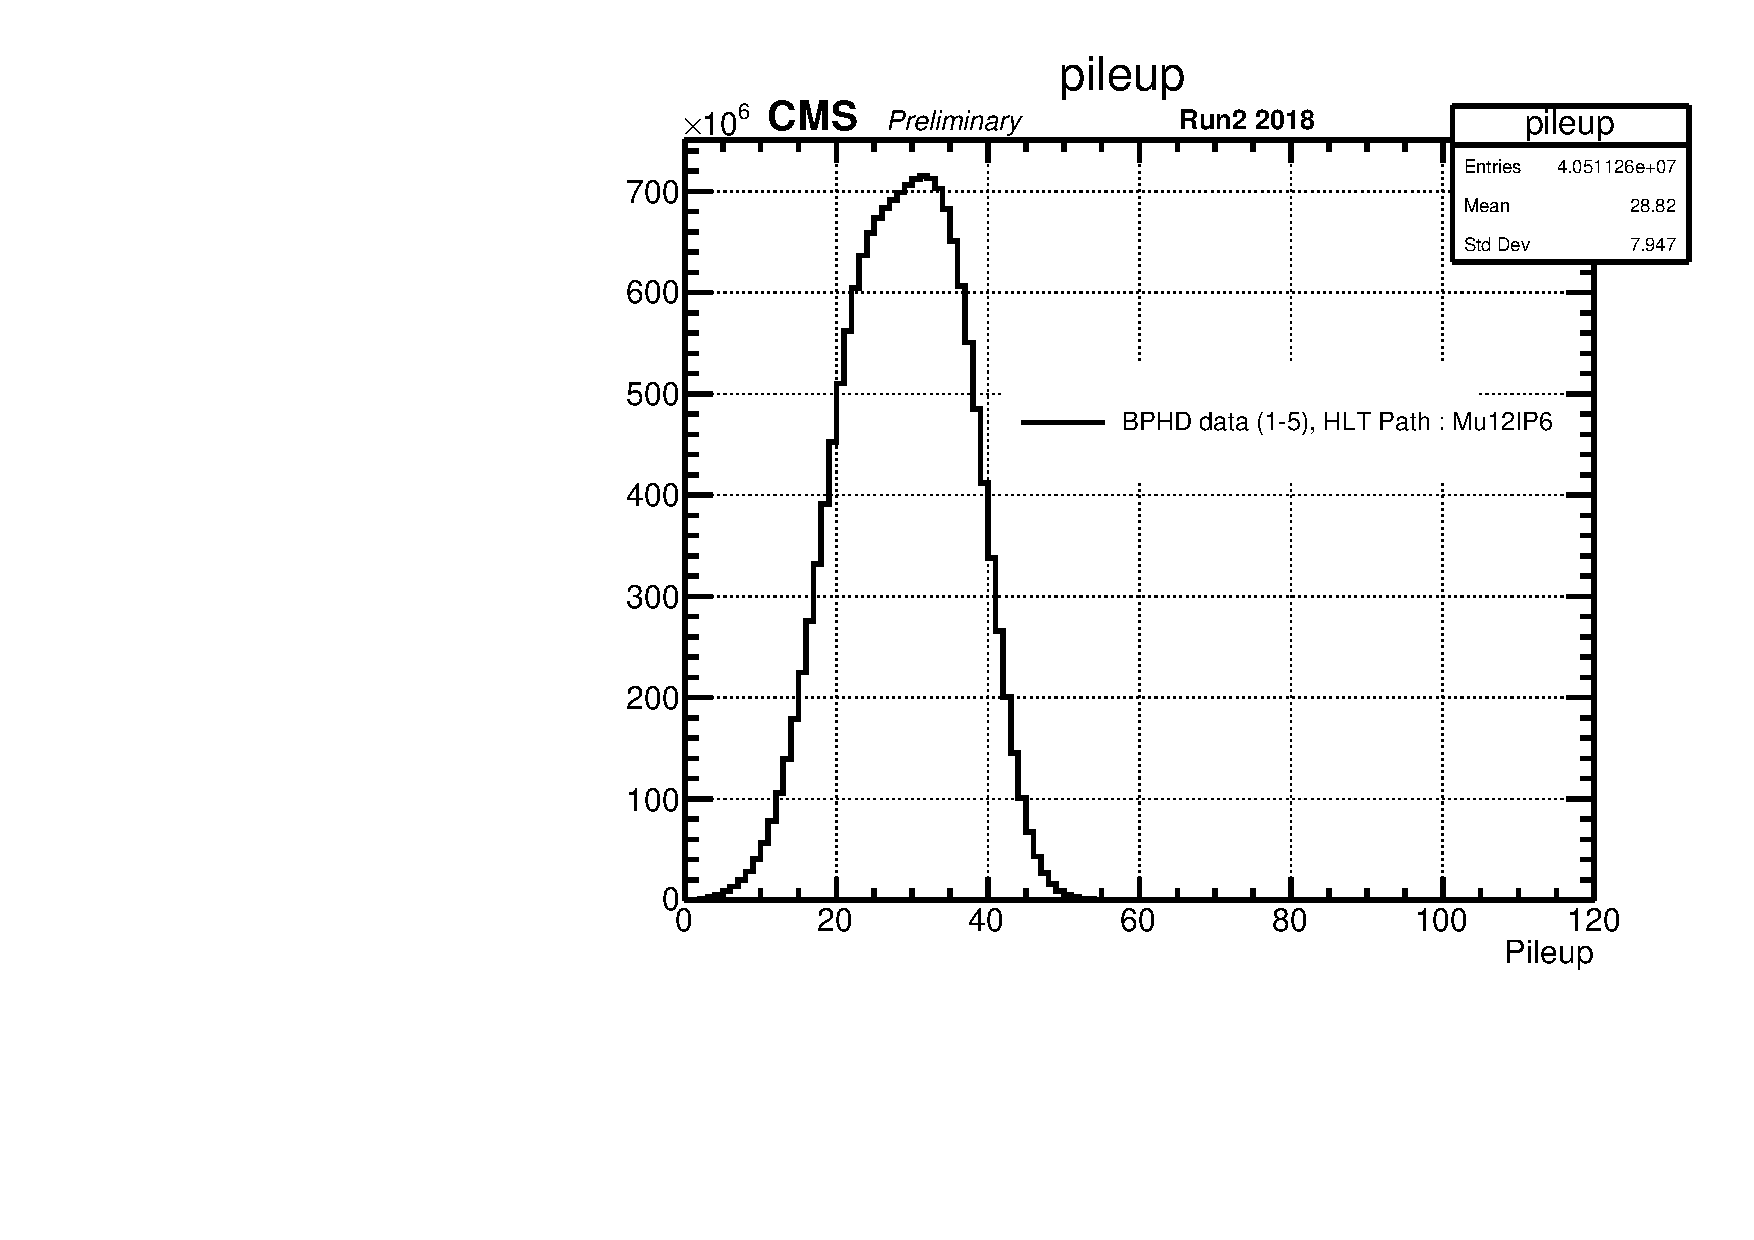
\includegraphics[width=0.57\linewidth]{figs/NVtx_BPHD.pdf}

\end{figure}

Figure~\ref{fig:MCPU} shows DYJetsToLL\_M-50\_TuneCP5\_13TeV-madgraphMLM-pythia8 MC PU distribution.
\begin{figure}[h!]
	\caption{Bunch crossing of Monte Carlo Simulation for physics process of Drell-Yan. The dataset is /DYJetsToLL\_M-50\_TuneCP5\_13TeV-madgraphMLM-pythia8
\newline/RunIISummer20UL18MiniAODv2-106X\_upgrade2018\_realistic\_v16\_L1v1-v2/\newline MINIAODSIM}
  \label{fig:MCPU}
  \centering
  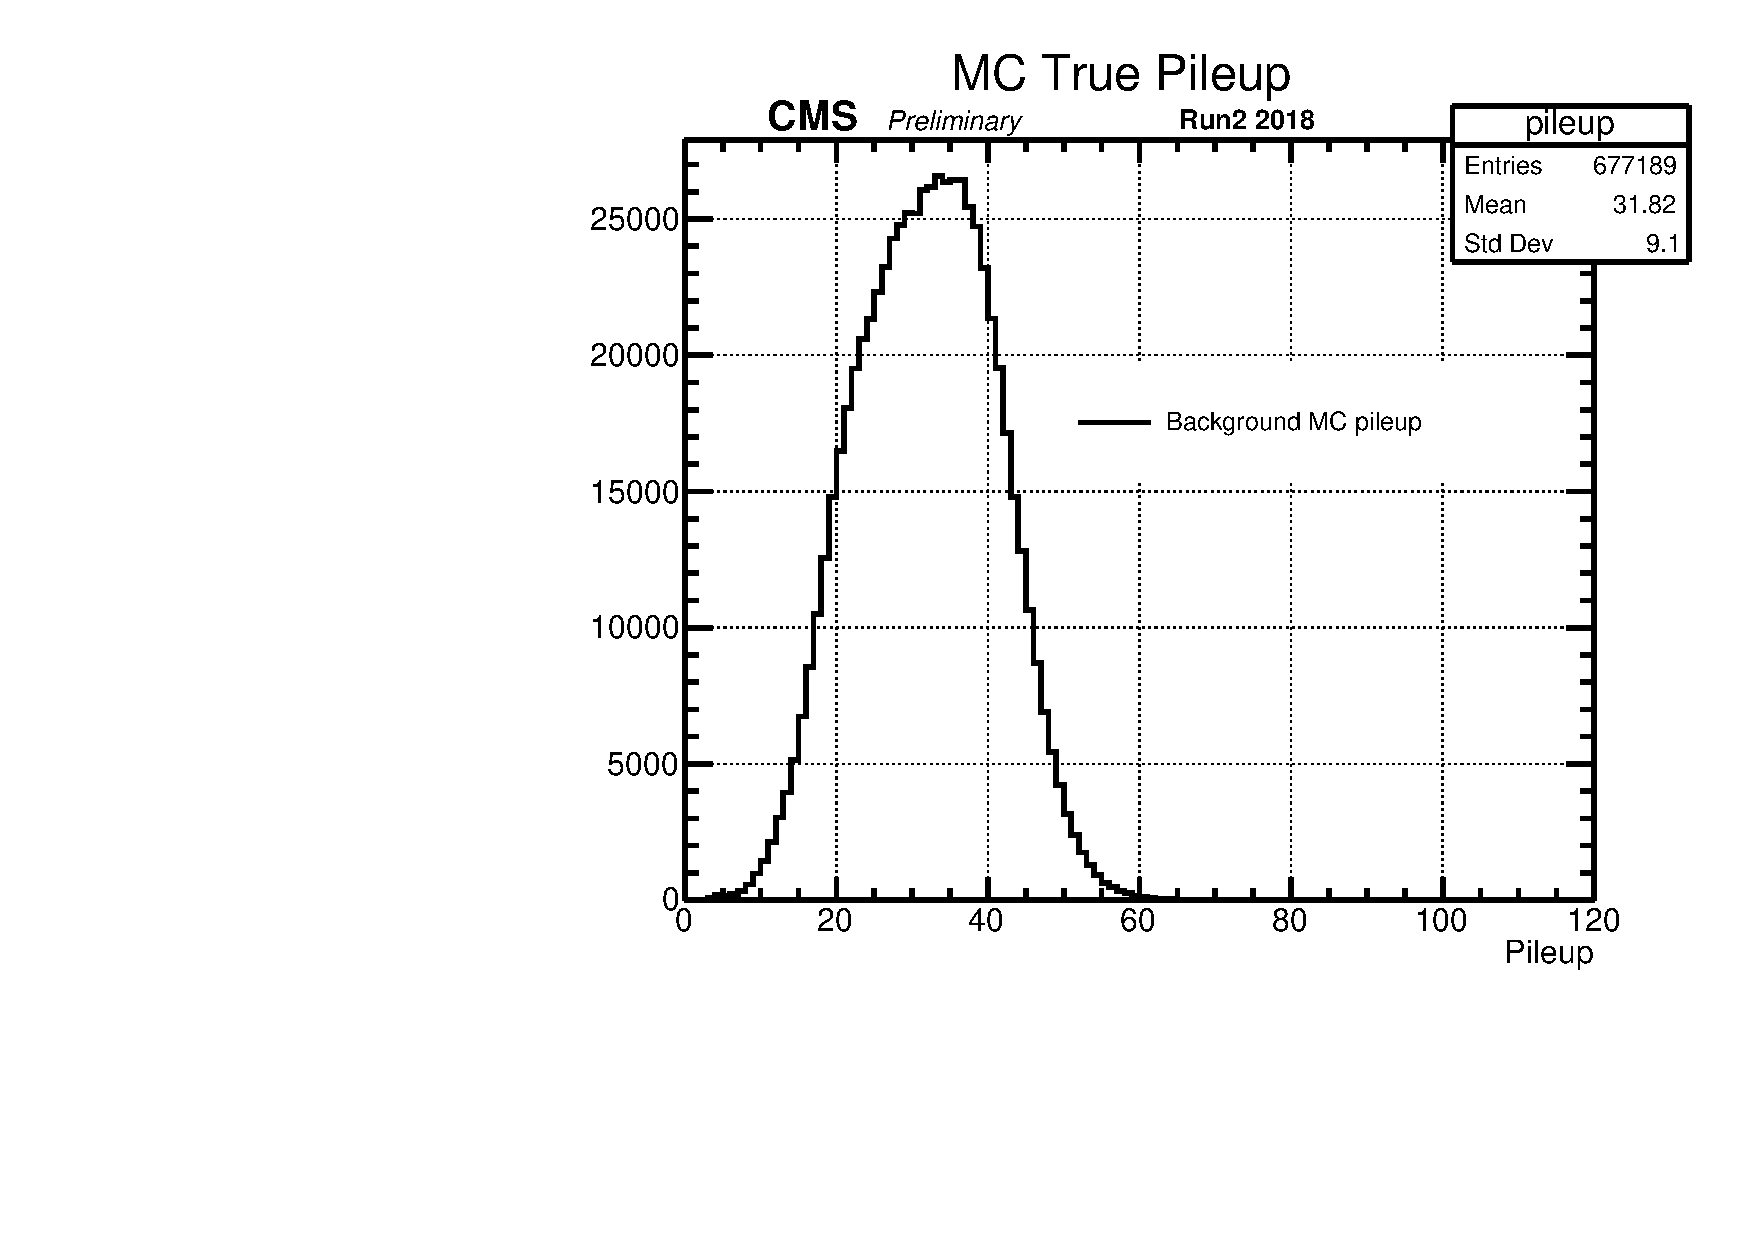
\includegraphics[width=0.67\linewidth]{figs/NVtx_DYJetsToLL_M-50_try.pdf}

\end{figure}

Figure~\ref{fig:PUWeight9} shows resultant such PUWeight from BPH1\_A HLT\_Mu9\_IP6 and DYJetsToLL\_M-50\_TuneCP5\_13TeV-madgraphMLM-pythia8.
\begin{figure}[h!]
  \caption{PUweight calculated for Era A of B-parking dataset}
  \label{fig:PUWeight9}
  \centering
  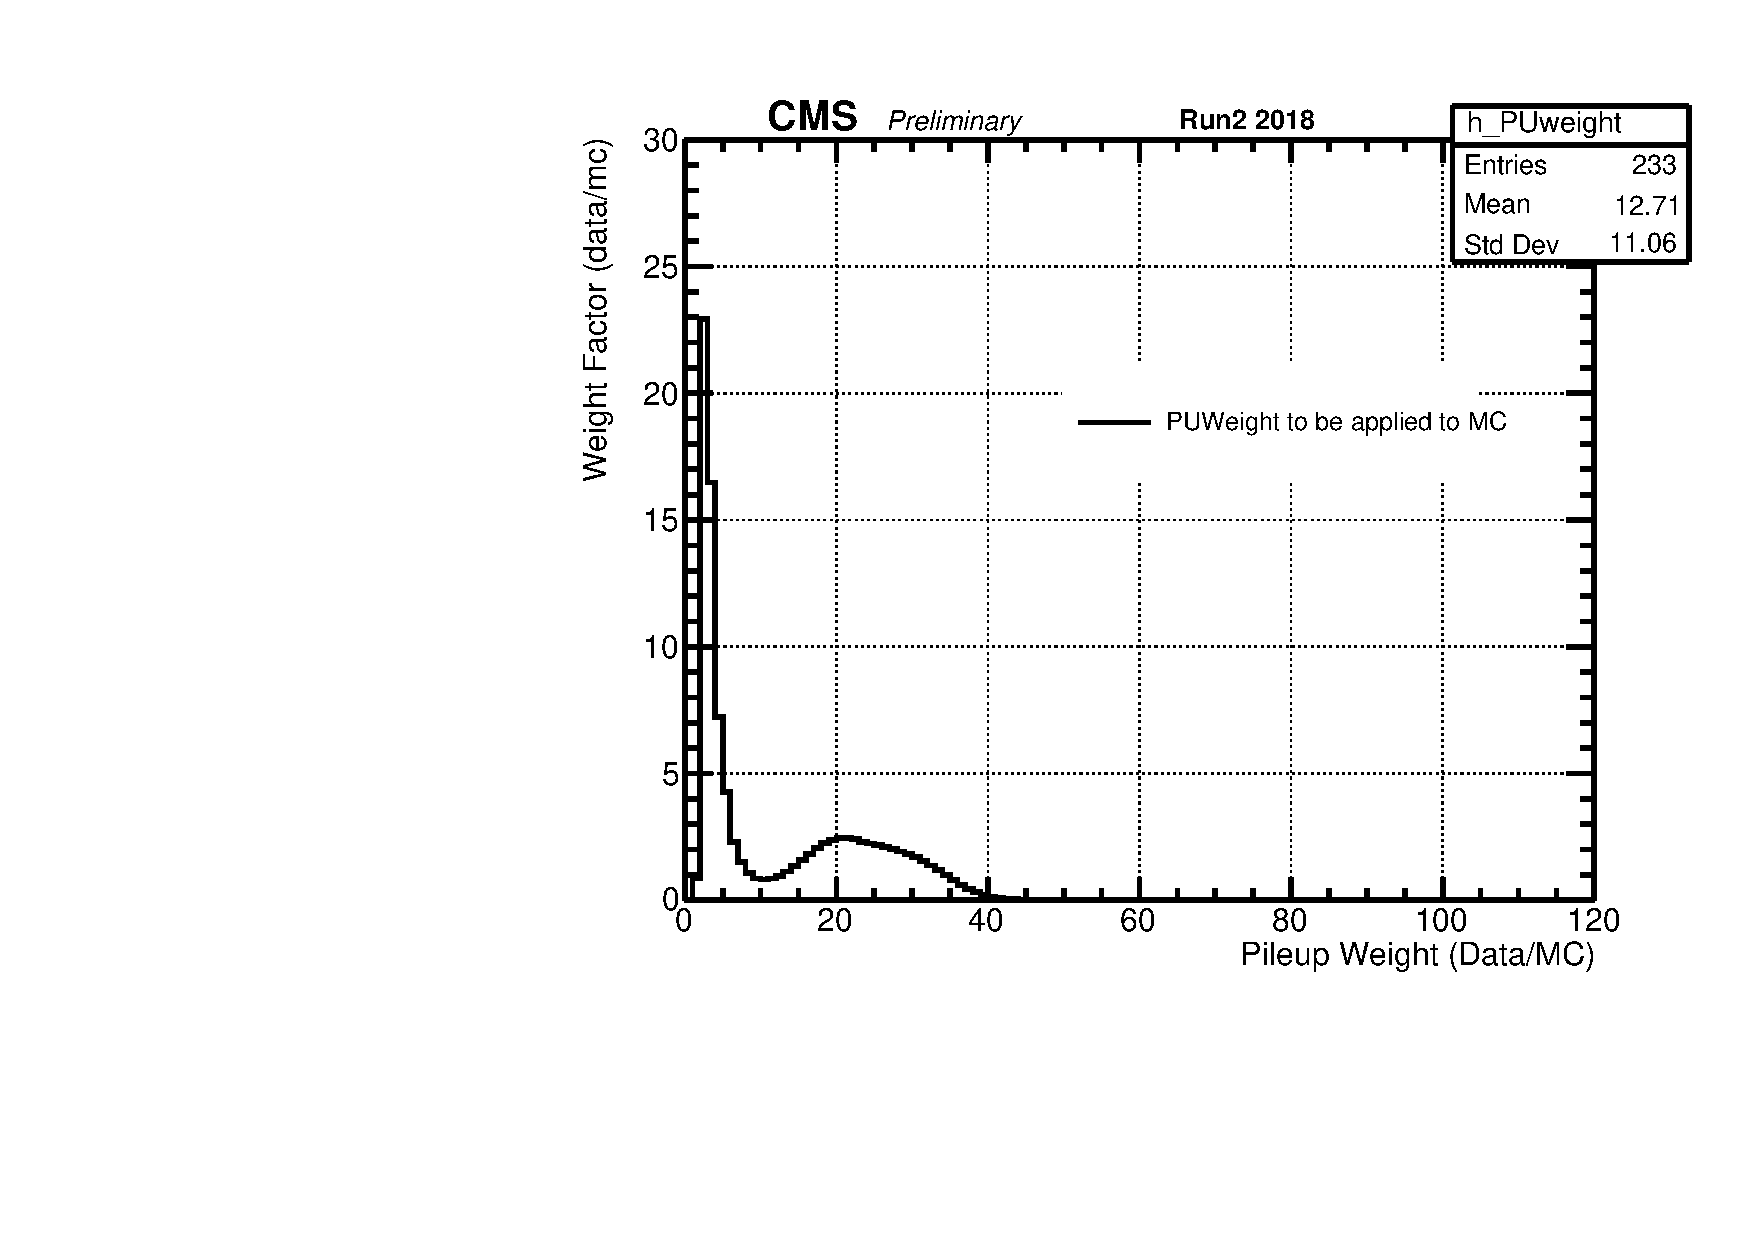
\includegraphics[width=0.67\linewidth]{figs/NVtx_PUWeight.pdf}

\end{figure}

\clearpage

\clearpage
\chapter{Physics Object Definitions}\label{sec:objects}
%reconstruction algorithms, isloation, cleaning, IDs, particle flow

This section provides the definitions of physics objects used in the analysis.
The analysis uses two main CMS reconstructed objects: muons and jets.
Photons do not show anywhere in our signal process.
$\tau$'s of our signal process can decay into electrons with the same probability as into muons.
However, the analysis uses b-parking and only targets the muon decay mode of the tau.
Electrons are not an interest of our analysis either.

Although the signal's final decay involves $\tau$ lepton, we do not use CMS reconstructed $\tau$.
Given that $\tau$ decay results in many different objects (muon, electron, and different combinations of hadrons) as shown in figure \ref{fig:tdecay}, CMS uses a special reconstruction algorithm for $\tau$ object.
Particle-Flow jets (PFjets), with all particle identification information within the jet, are the starting point for the $\tau$ reconstruction.
With $\pi^{0}$ reconstructed in ECAL as a strip, the Hadronic-Plus-Strip (HPS) algorithm reconstructs $\tau$ (at 60\% efficiency in Run 1) when a charged hadron and a strip are reconstructed in the PFJet \cite{HPS}.
Our signal process tau lepton decays into muon, in a leptonic mode, for the trigger.
We approach a tracker-oriented method with regions of interest to analyze other tau leptons in the signal process.
Direct usage of tau leptons in the analysis is accompanied by a division of several different sub-channels ($\mu$,e, had), which result in 27 ($3^{3}$) different combinatorics.

We use muon leptons, jets, and only tracks (ROIs) for this analysis.
\section{Muons}\label{sec:muons}
The analysis sources the SlimmedMuons collection from the MINIAOD MC datasets to produce {\tt selectedPatMuons}.
Muon objects are required to have 
\begin{itemize}
  \item $pT$ $\geq$ 12 GeV to reach BPH trigger plateau
  \item $|\eta|$ $\leq$ 1.5 for L1 seed $|\eta|$ cut in BPH trigger
  \item reco::Muon object matched to the BPH trigger object
  \item Pass the Loose ID criterion (isLooseMuon) as described in the Muon POG~\cite{muonpog}.
\end{itemize}

\begin{figure}[h!]
  \caption{Data/MC of muon objects pT, $\eta$, energy, nMu}
  \label{fig:muons}
  \centering
  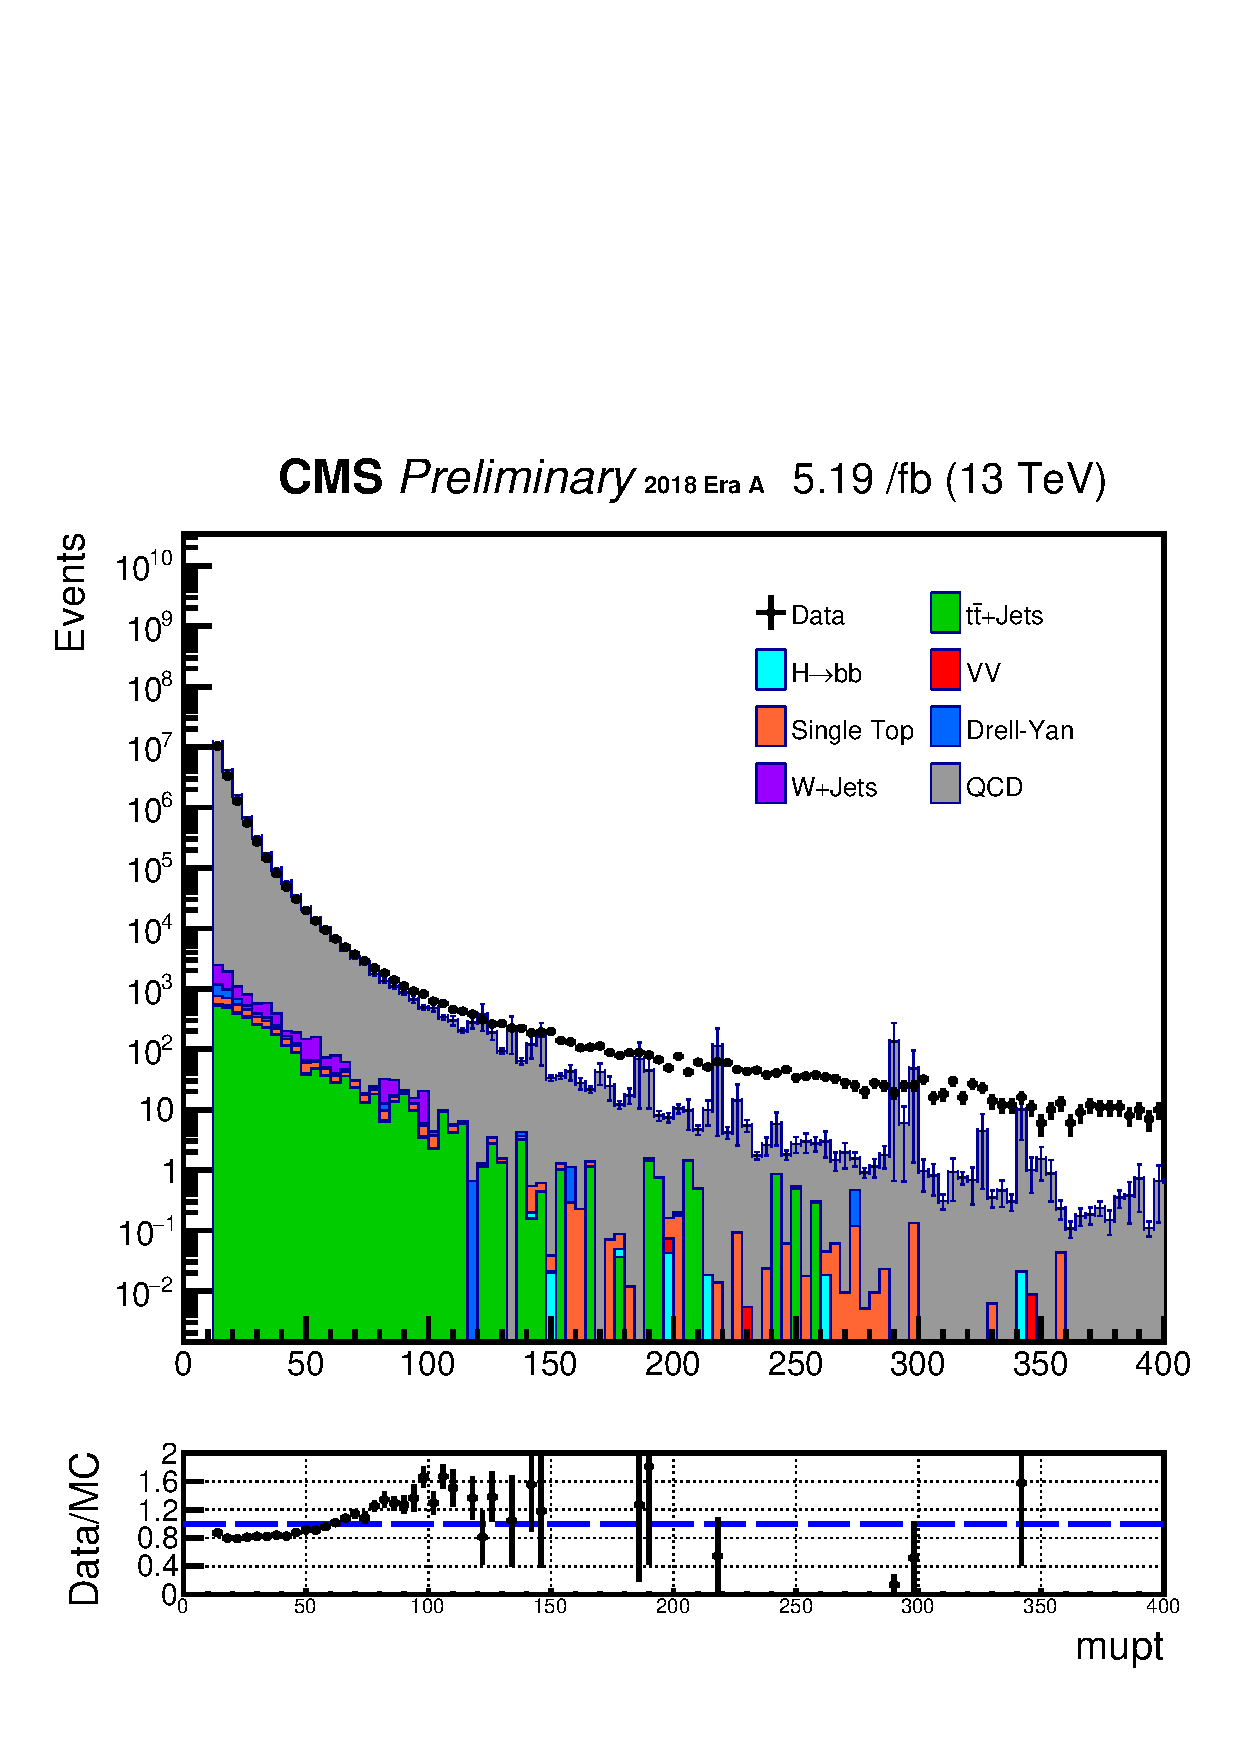
\includegraphics[width=0.47\linewidth]{figs/Data_log_AnalysisNote_MS-15_ctauS-10_mupt.pdf}
  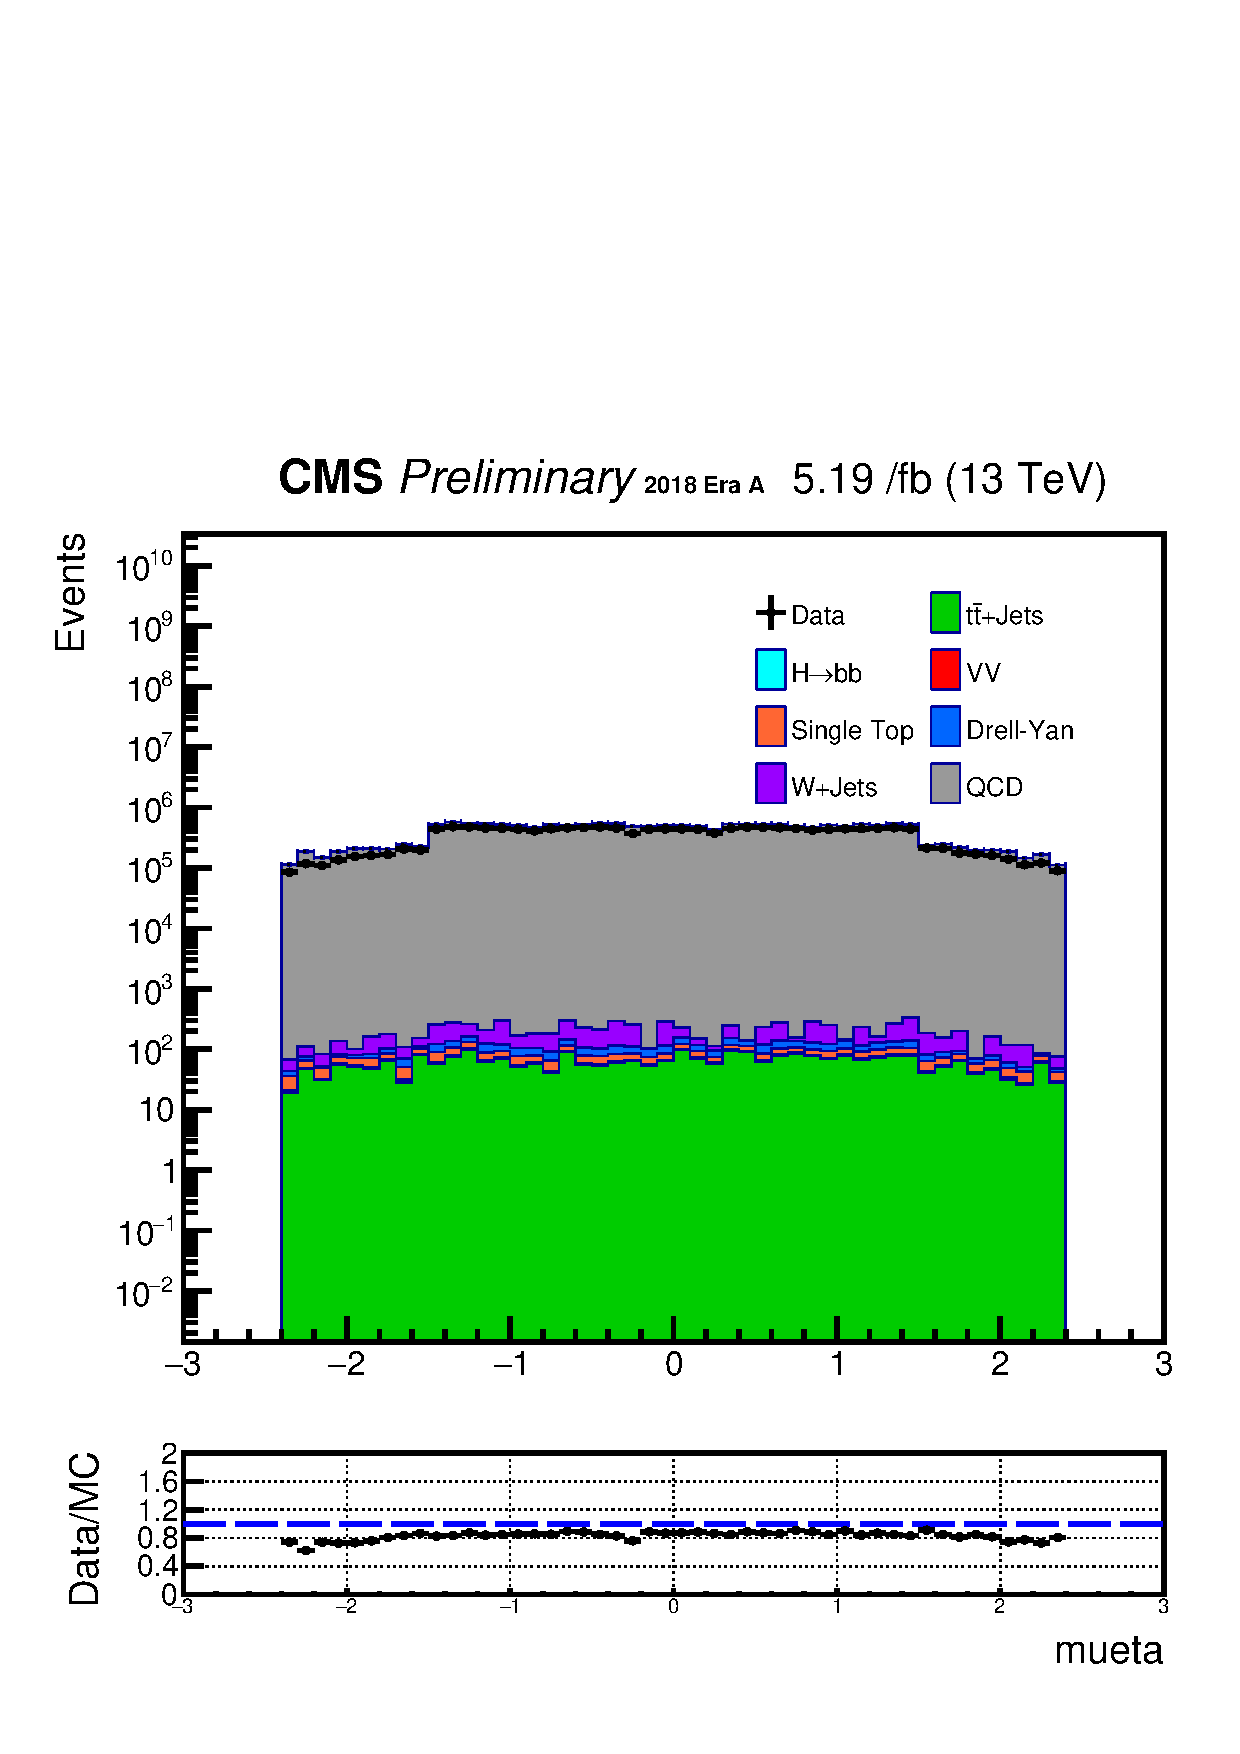
\includegraphics[width=0.47\linewidth]{figs/Data_log_AnalysisNote_MS-15_ctauS-10_mueta.pdf}
  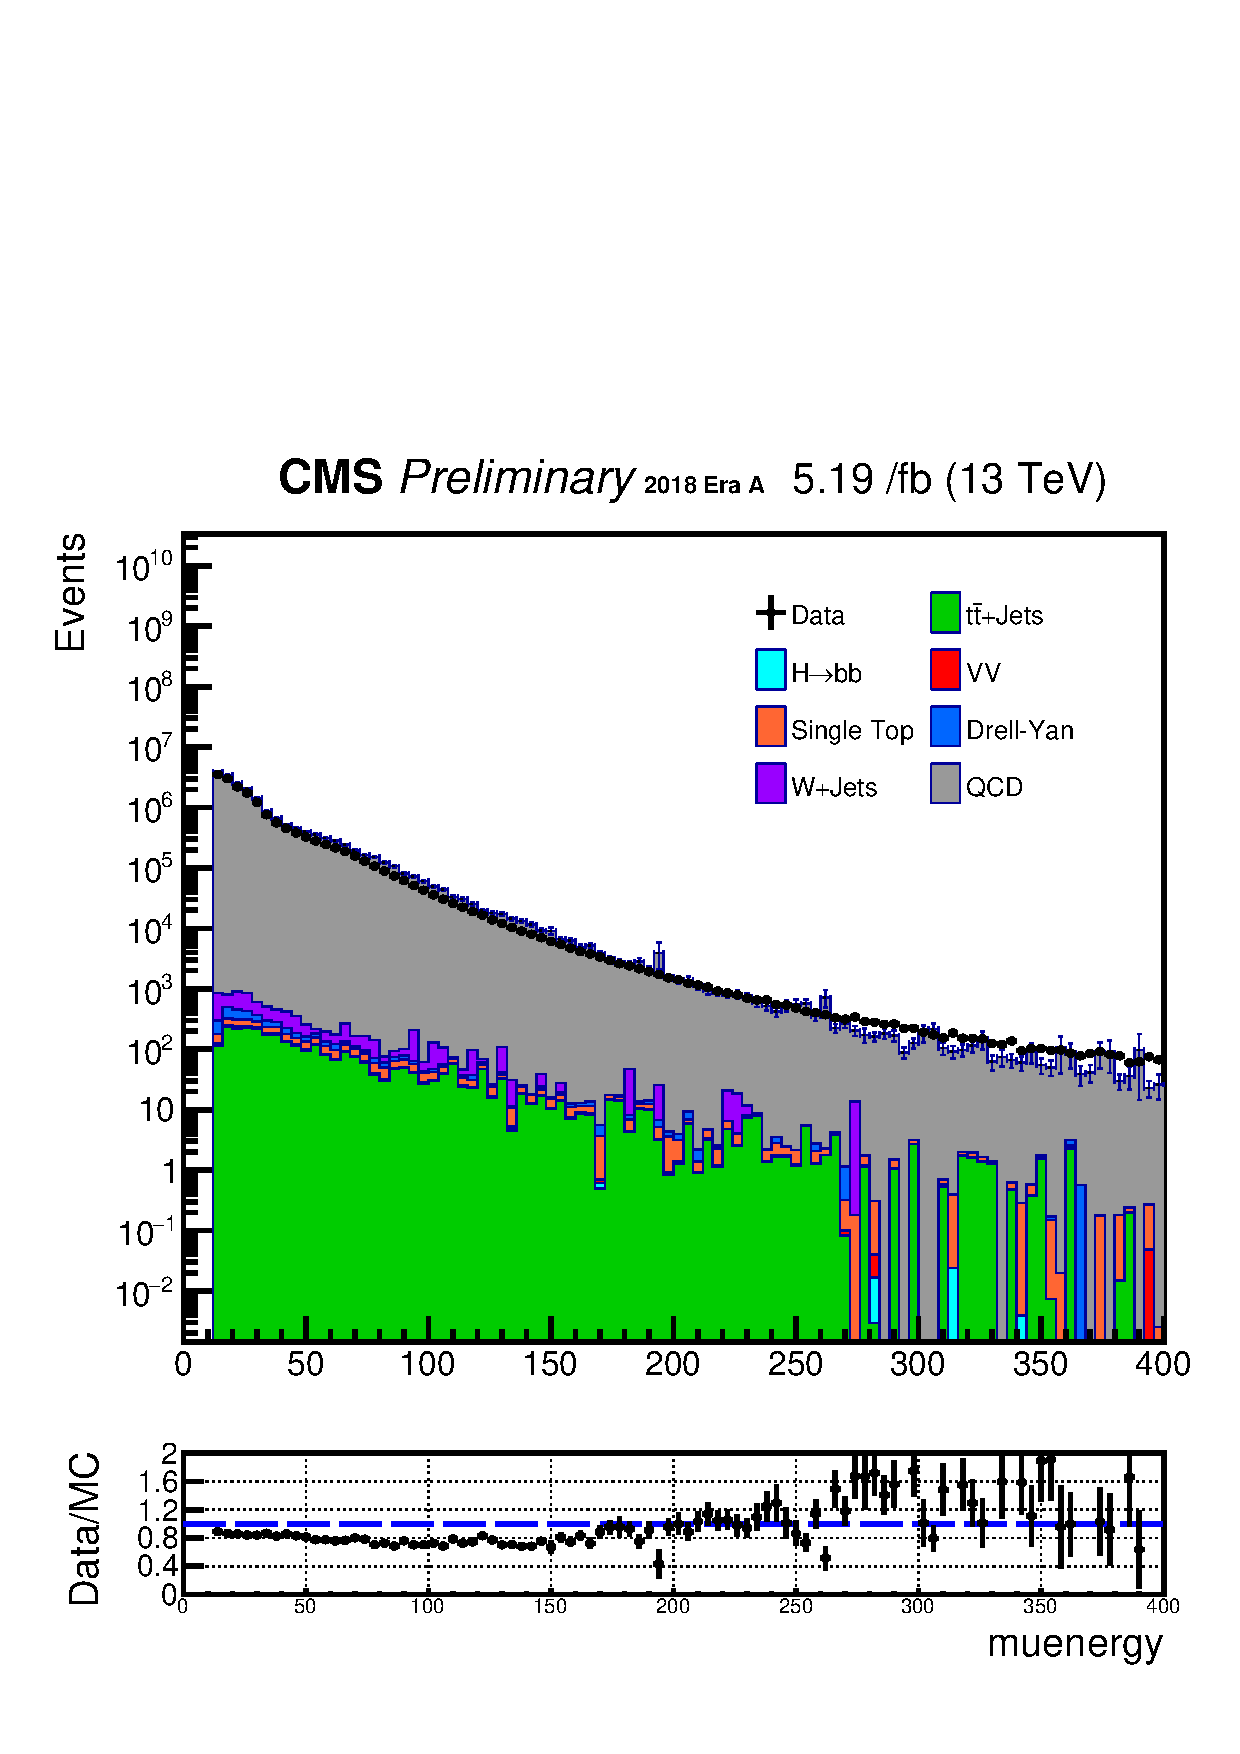
\includegraphics[width=0.47\linewidth]{figs/Data_log_AnalysisNote_MS-15_ctauS-10_muenergy.pdf}
  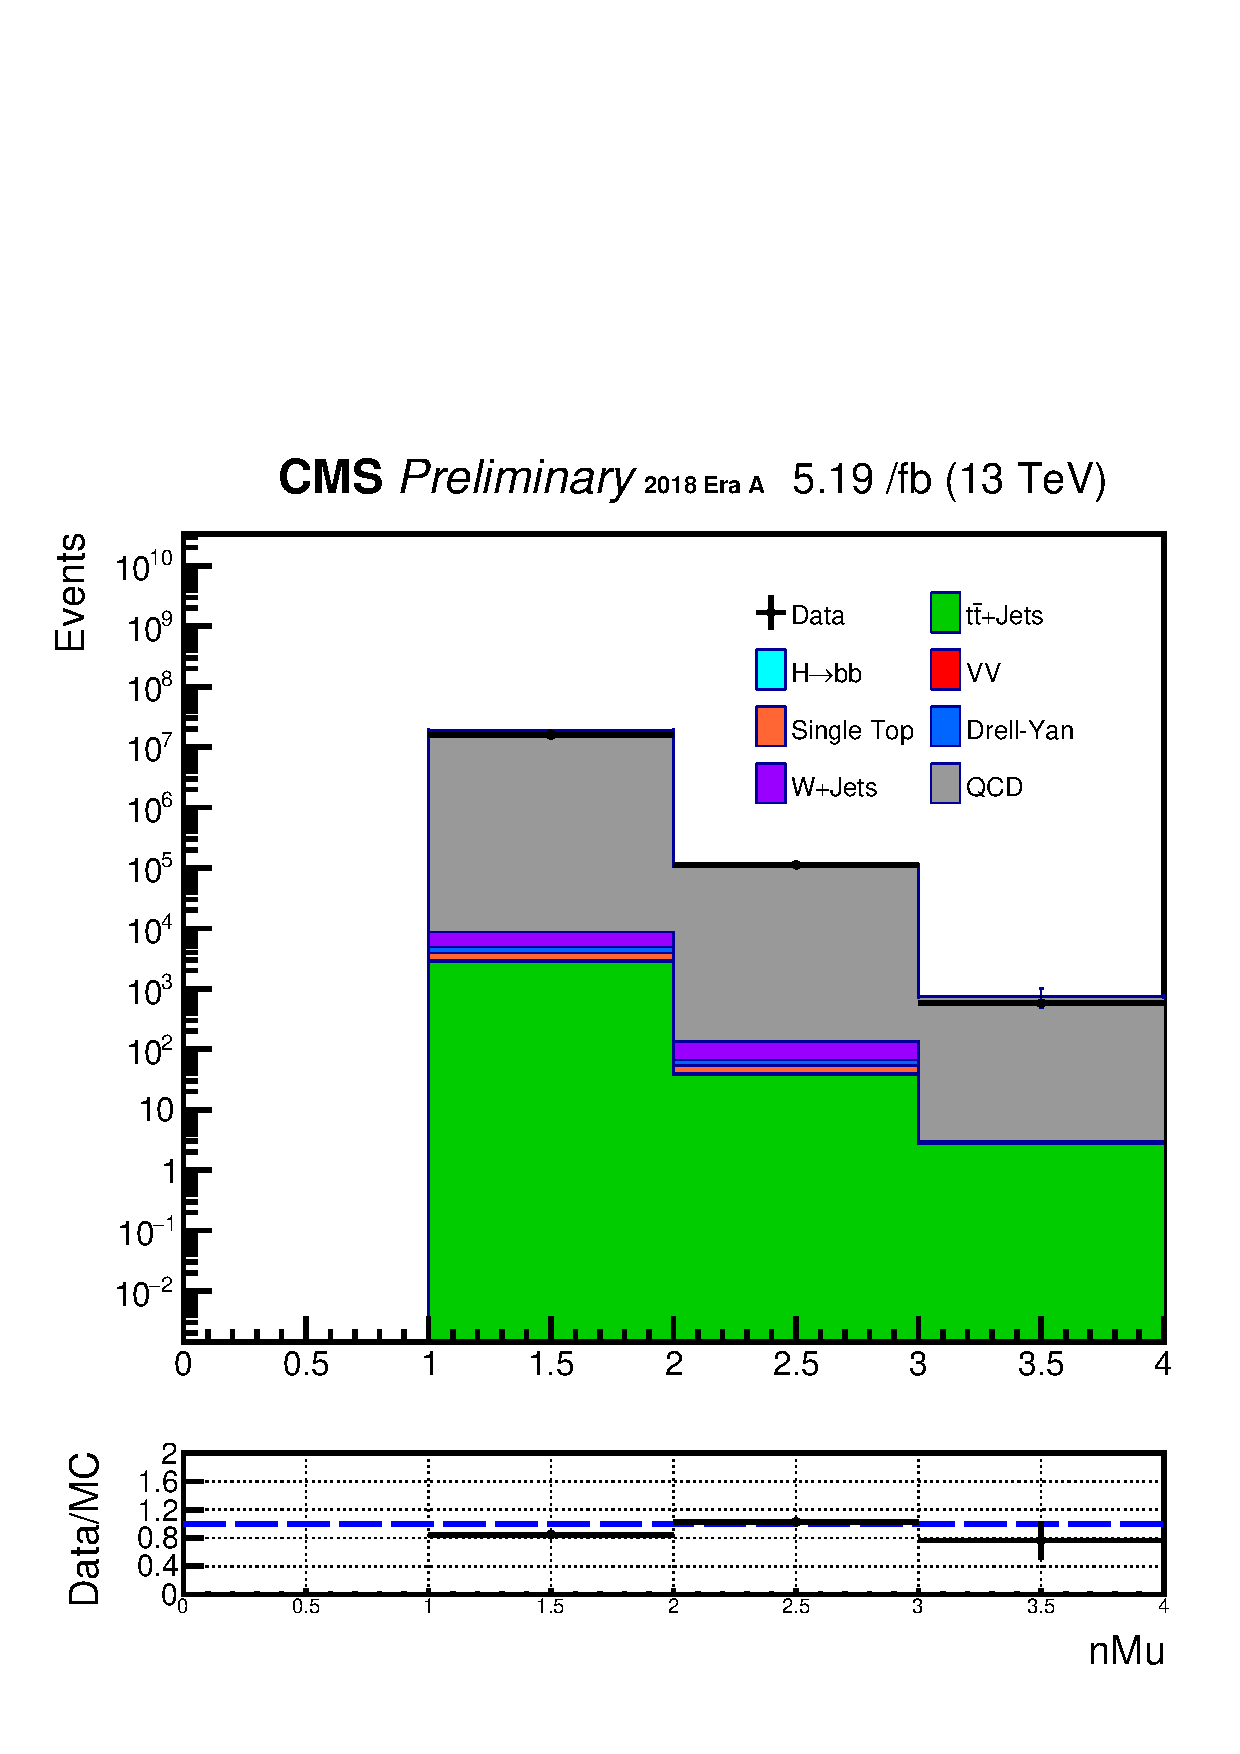
\includegraphics[width=0.47\linewidth]{figs/Data_log_AnalysisNote_MS-15_ctauS-10_nMu.pdf}
\end{figure}

The motivations for isolation requirements on muons are further discussed in Section~\ref{sec:selections}.


\section{Jets}\label{sec:jets}
The analysis sources SlimmedJets collection from MINIAOD dataset to produce {\tt selectedJets}.
CMS reconstructs jets from calorimeter energy deposits using the
anti-$k_T$ clustering algorithm with a distance parameter of $R=0.4$~\cite{Cacciari:2008gp}.
Then, the calojets are input into the Particle-Flow (PF) algorithms to produce the PFJets collection. Then, variables in PFJets class are slimmed to be saved into MINIAOD files.
%The analysis uses these SlimmedJets for the jets' b tagging scores as well.
Jet objects require
\begin{itemize}
  \item pt $\geq$ 20 GeV
  \item $|\eta|$ $\leq$ 2.4
  \item 0 $\leq$ emEnergyFraction $\leq$ 0.9
  \item 0 $\leq$ energyFractionHadronic $\leq$ 0.9
  \item No selected electron or muon within $\Delta R=0.4$
\end{itemize}
The energy fraction cuts above are taken from the recommended Run2 Tight jet ID
cuts for particle flow jets~\cite{jetid_2018}.
\begin{figure}[h!]
  \caption{Data/MC of jet objects for pT, $\eta$, energy, nJet}
  \label{fig:jets}
  \centering
  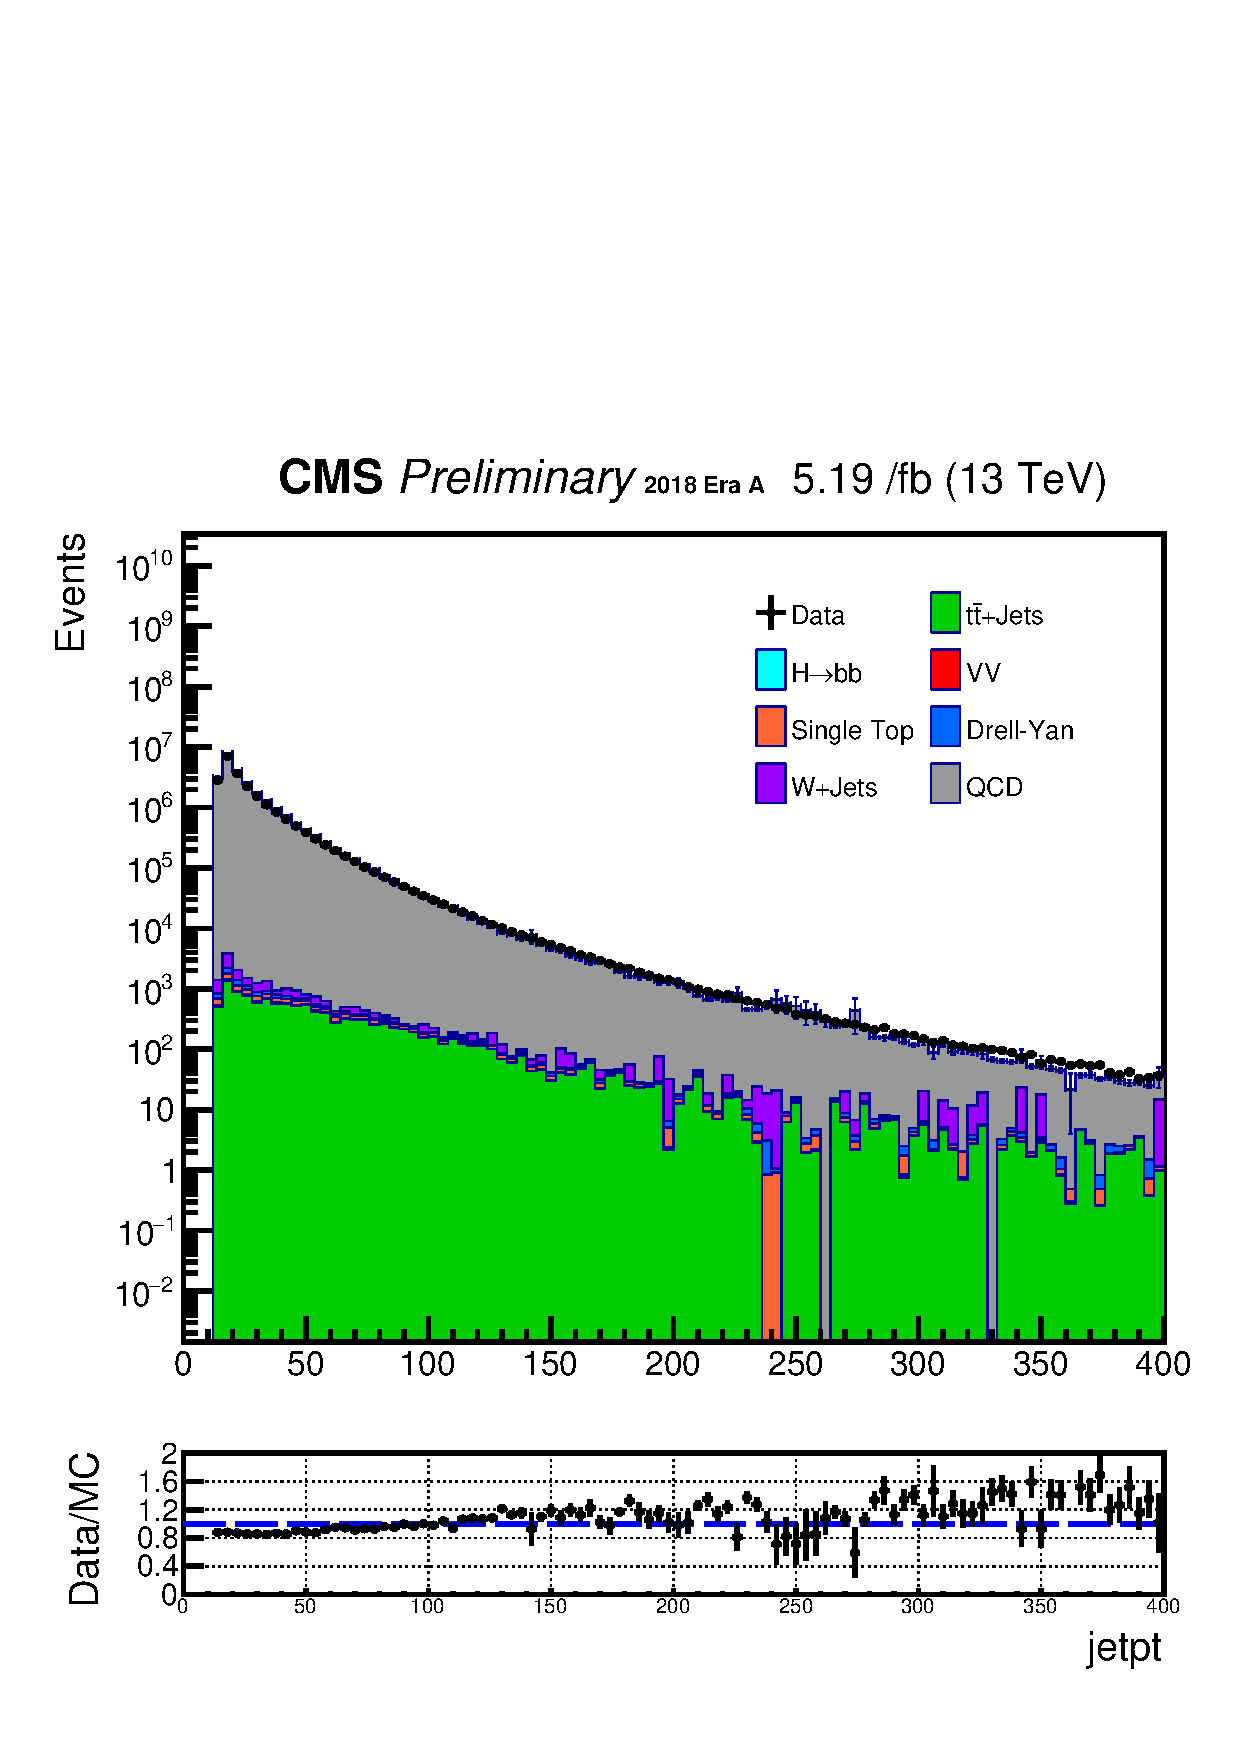
\includegraphics[width=0.47\linewidth]{figs/Data_log_AnalysisNote_MS-15_ctauS-10_jetpt.pdf}
  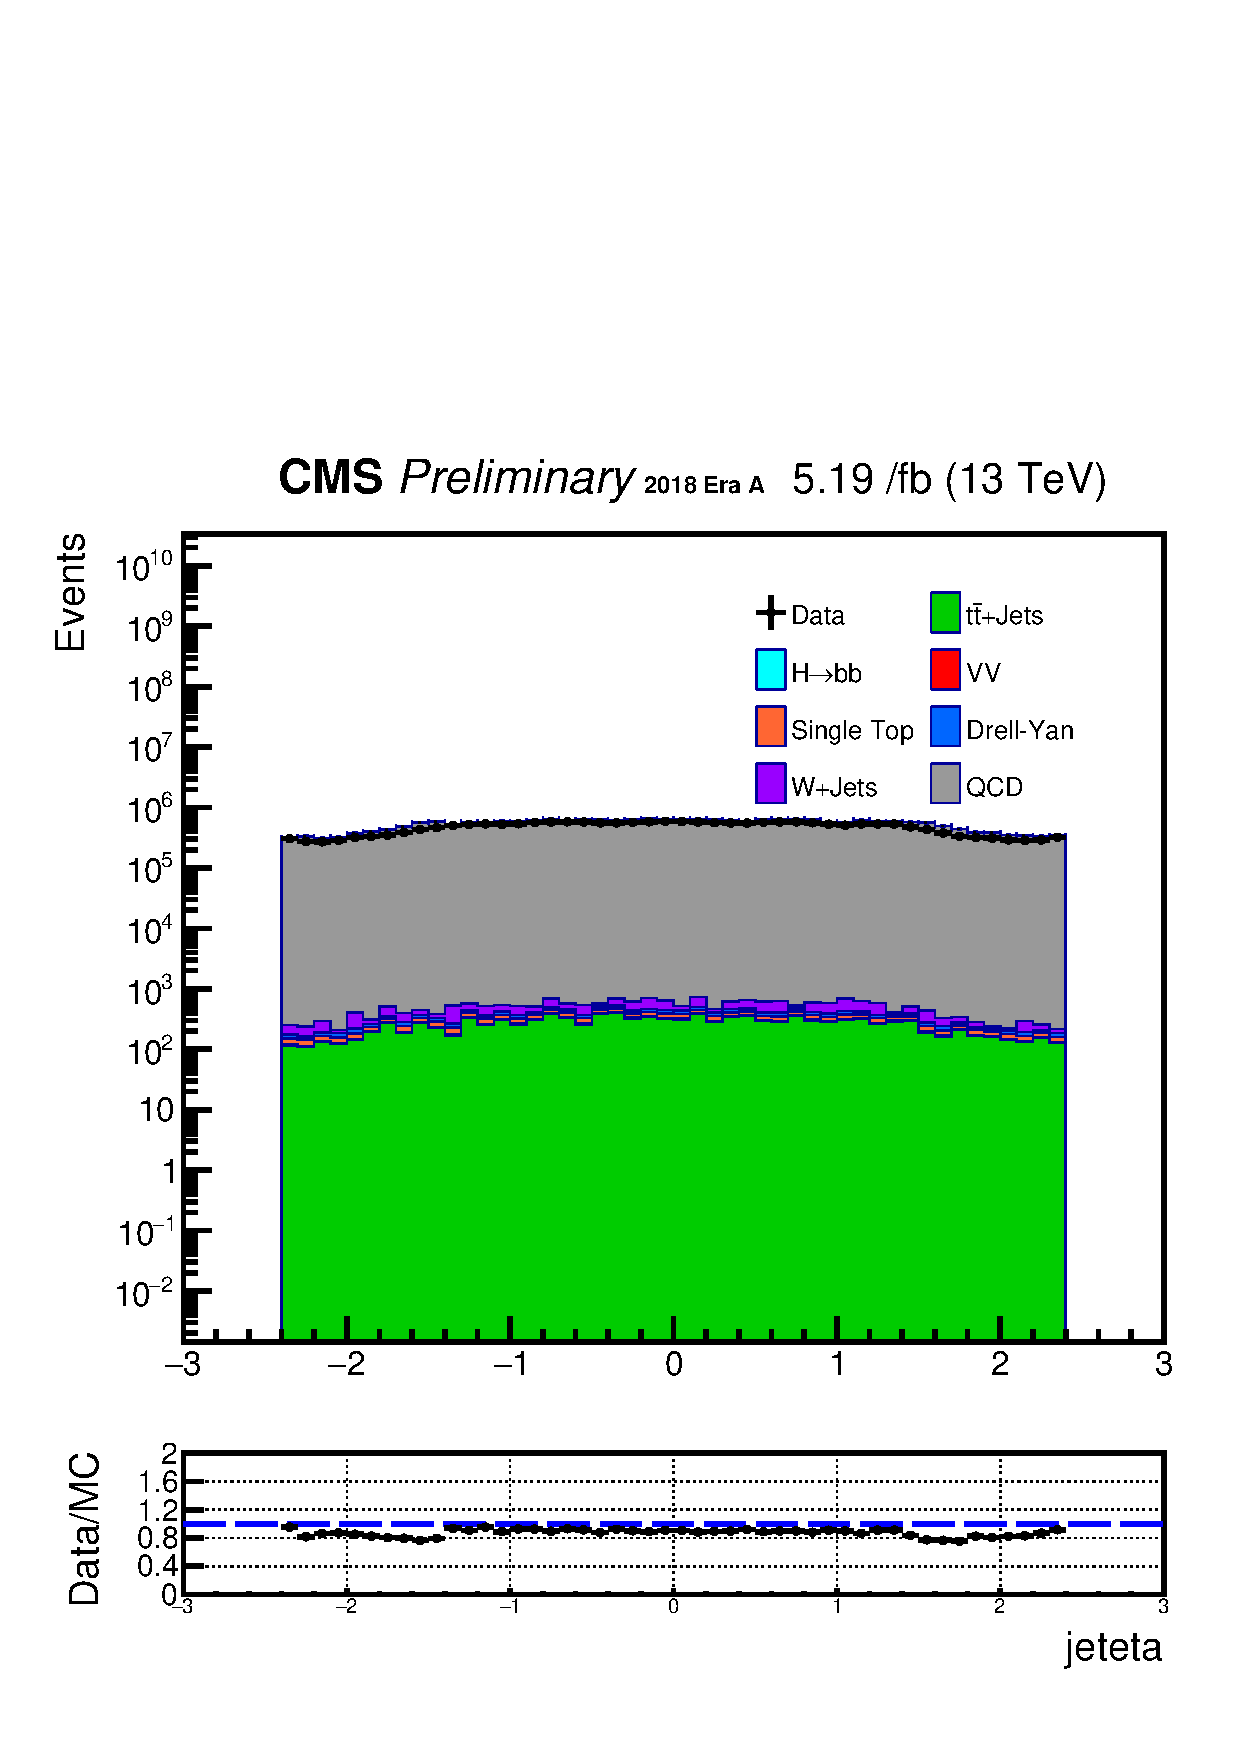
\includegraphics[width=0.47\linewidth]{figs/Data_log_AnalysisNote_MS-15_ctauS-10_jeteta.pdf}
  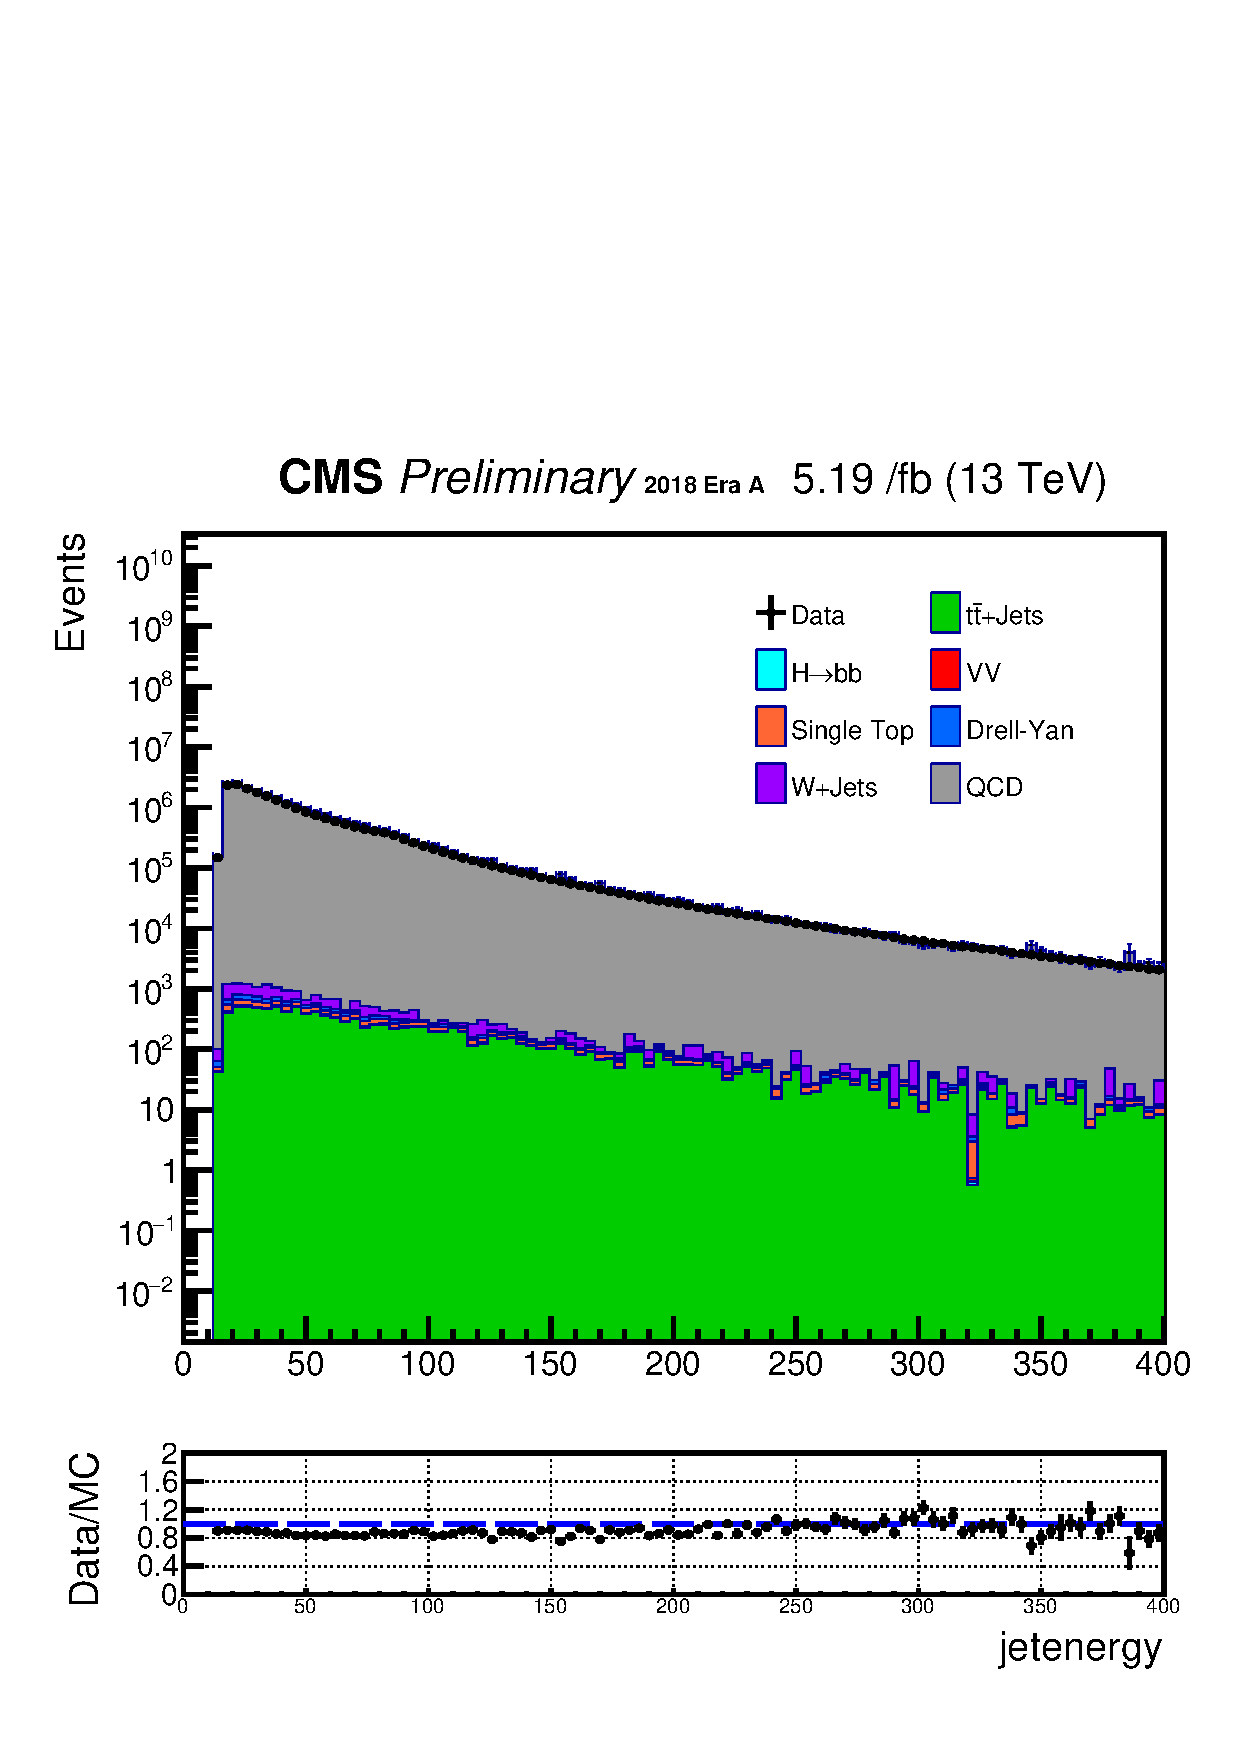
\includegraphics[width=0.47\linewidth]{figs/Data_log_AnalysisNote_MS-15_ctauS-10_jetenergy.pdf}
  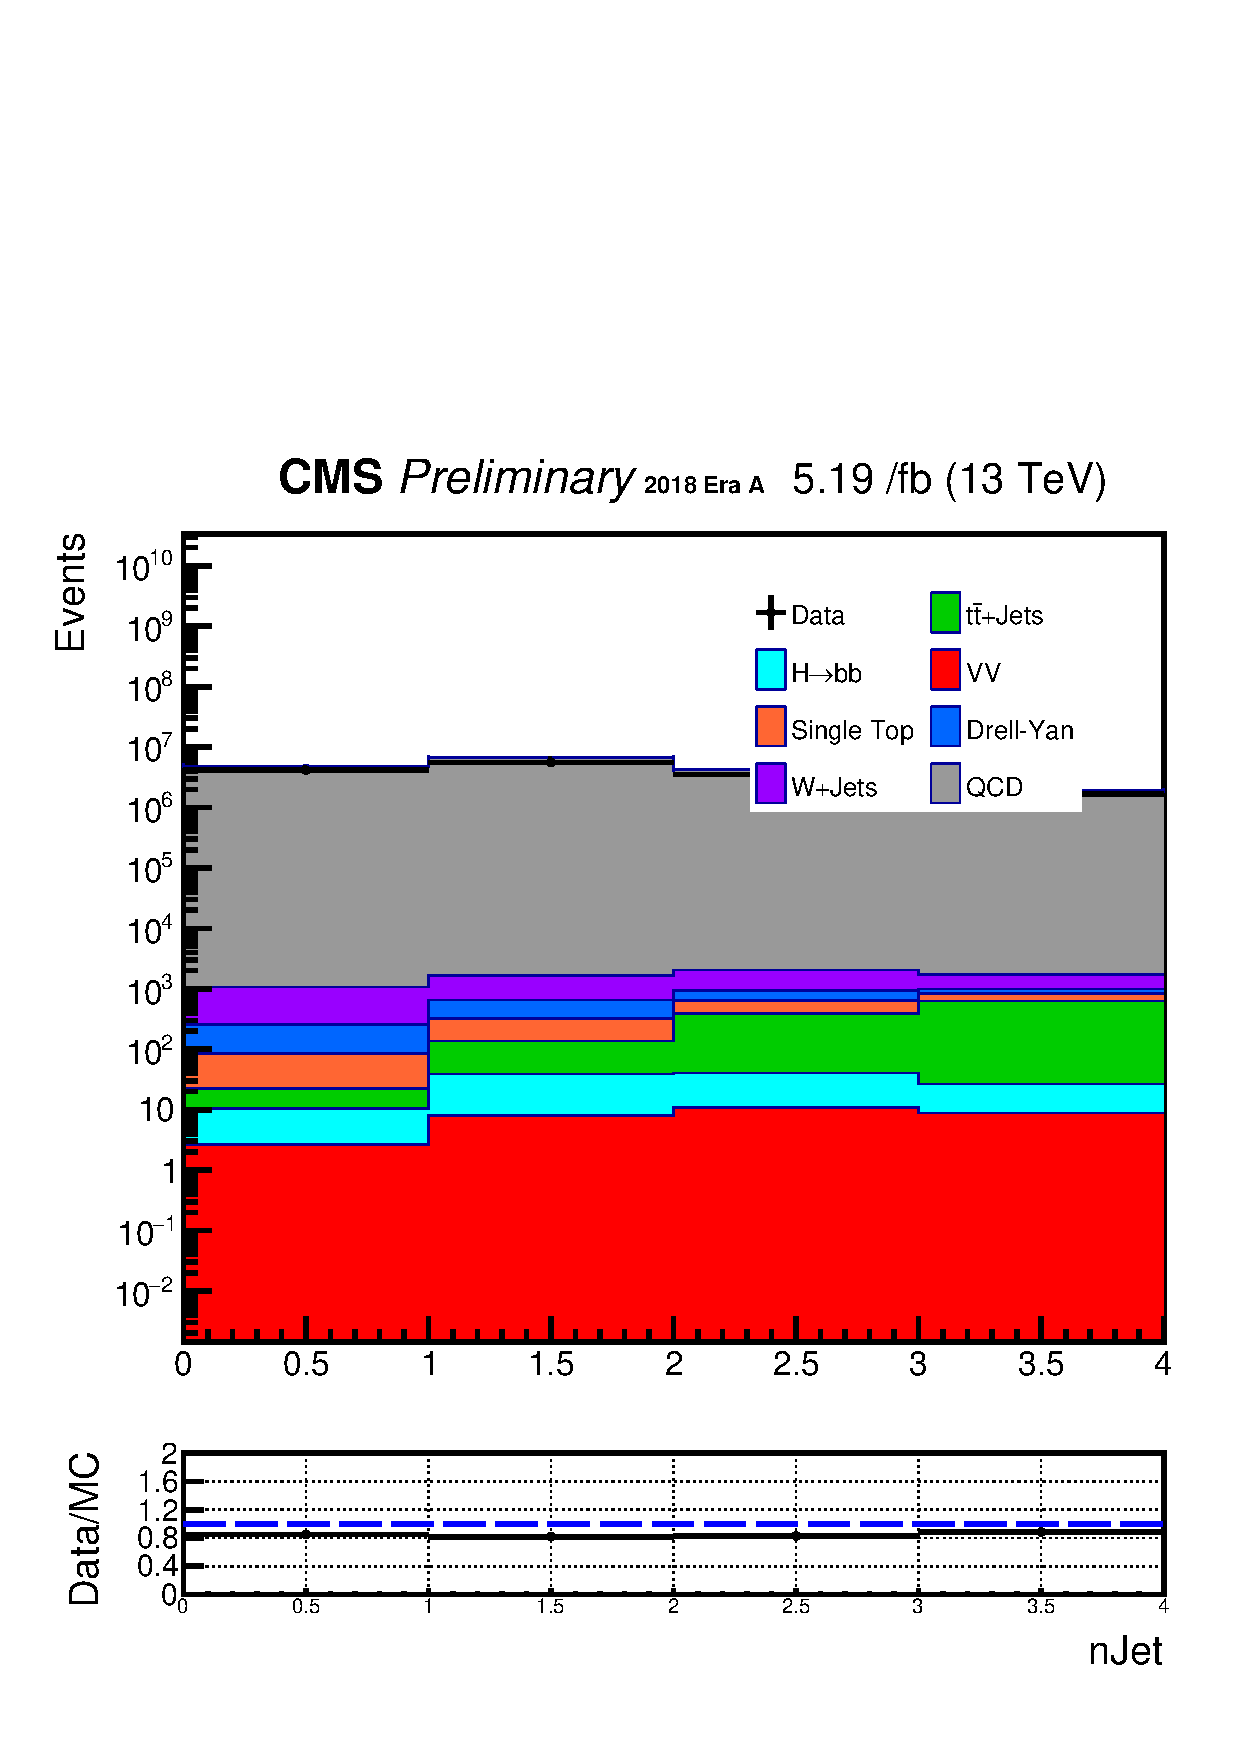
\includegraphics[width=0.47\linewidth]{figs/Data_log_AnalysisNote_MS-15_ctauS-10_nJet.pdf}
\end{figure}

\section{Taus}\label{sec:taus}
Although we do not use tau leptons for event selection or background estimation, we still plotted essential variables of tau leptons for review.
The analysis sources PAT::slimmedTaus from MINIAOD for MC and RECO::slimmedTaus for Data to produce {\tt selectedTaus}.
$\tau$'s hadronic decay can be reconstructed with PFJets' charged hadrons in HCAL, and 2 $\gamma$s from $\pi^{0}$ decays in ECAL.
Tau objects require
\begin{itemize}
  \item pt $\geq$ 20 GeV
  \item $|\eta|$ $\leq$ 2.4
\end{itemize}

\begin{figure}[h!]
  \caption{Data/MC of tau objects for pT, $\eta$, energy, nJet}
  \label{fig:taus}
  \centering
  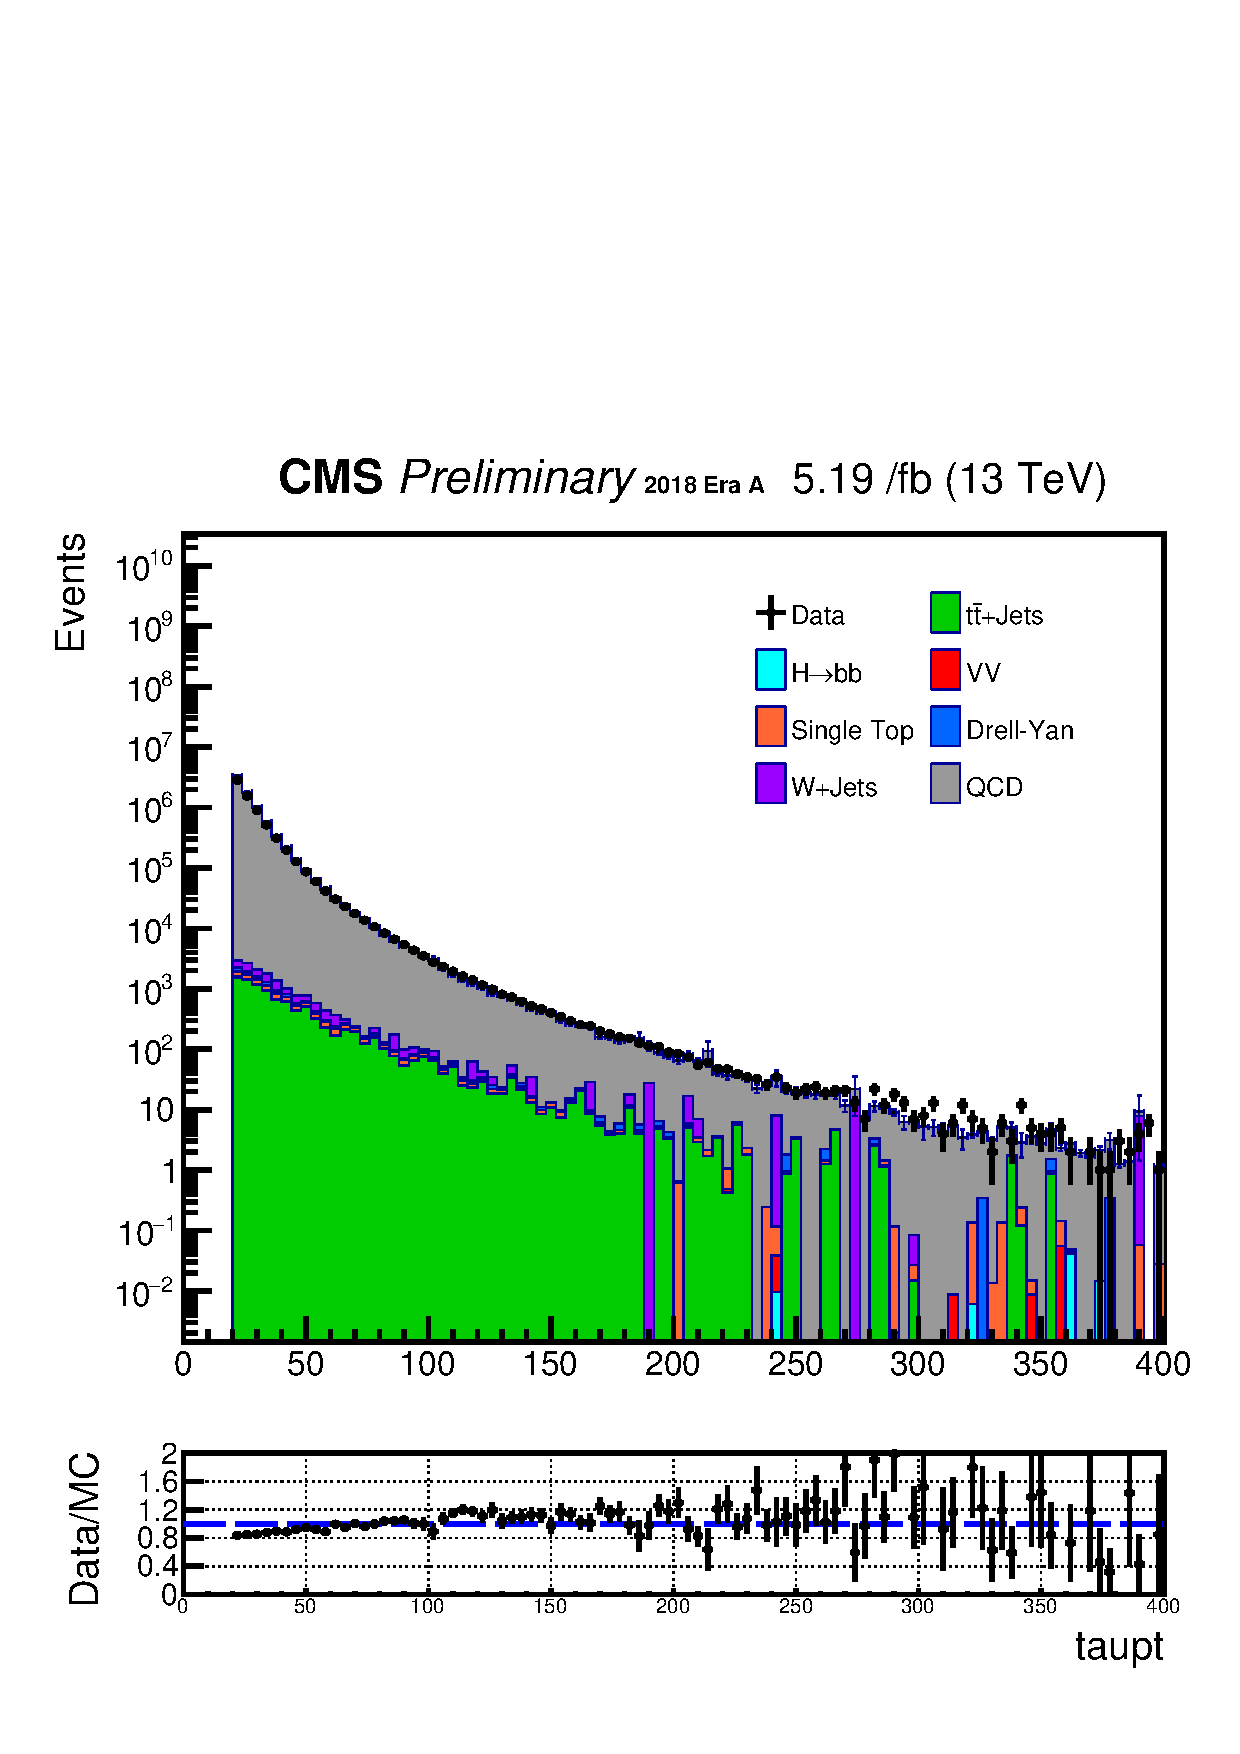
\includegraphics[width=0.47\linewidth]{figs/Data_log_AnalysisNote_MS-15_ctauS-10_taupt.pdf}
  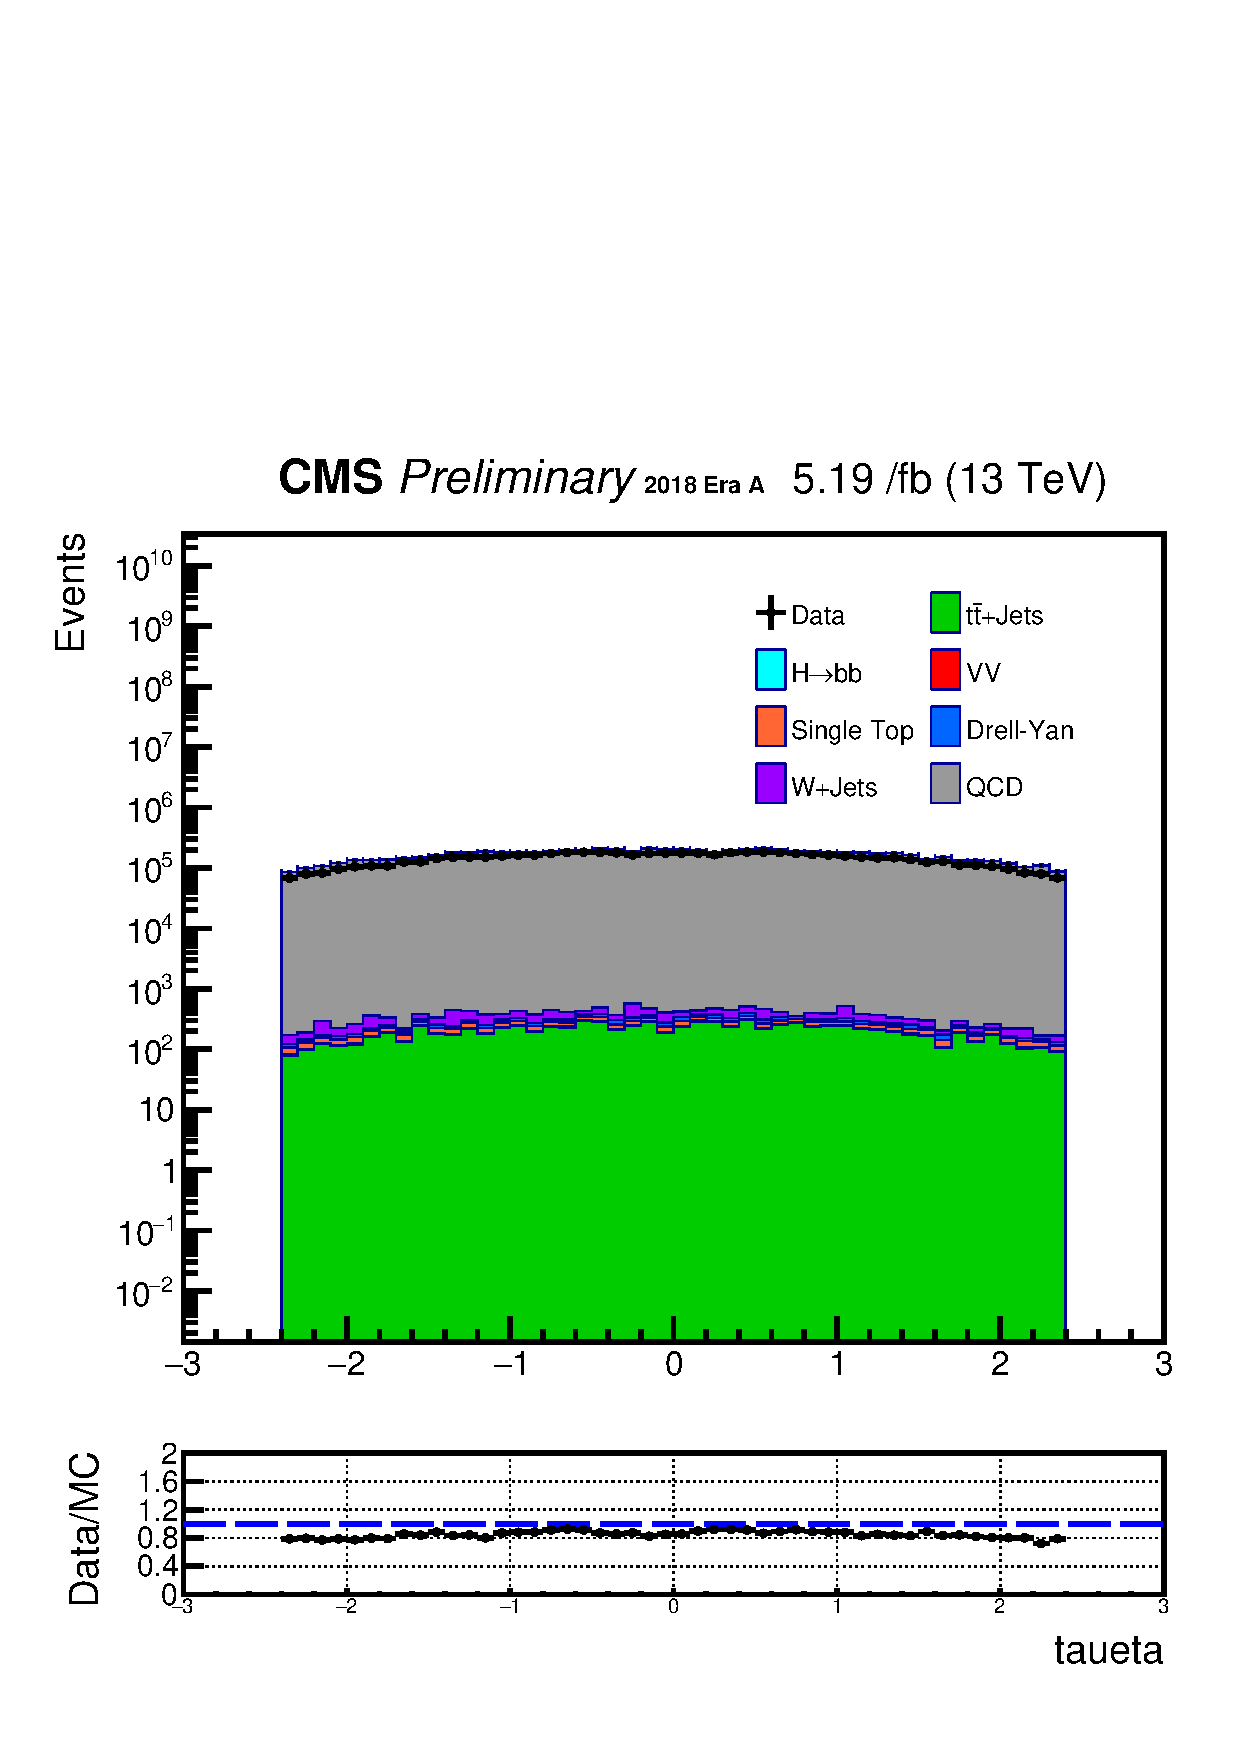
\includegraphics[width=0.47\linewidth]{figs/Data_log_AnalysisNote_MS-15_ctauS-10_taueta.pdf}
  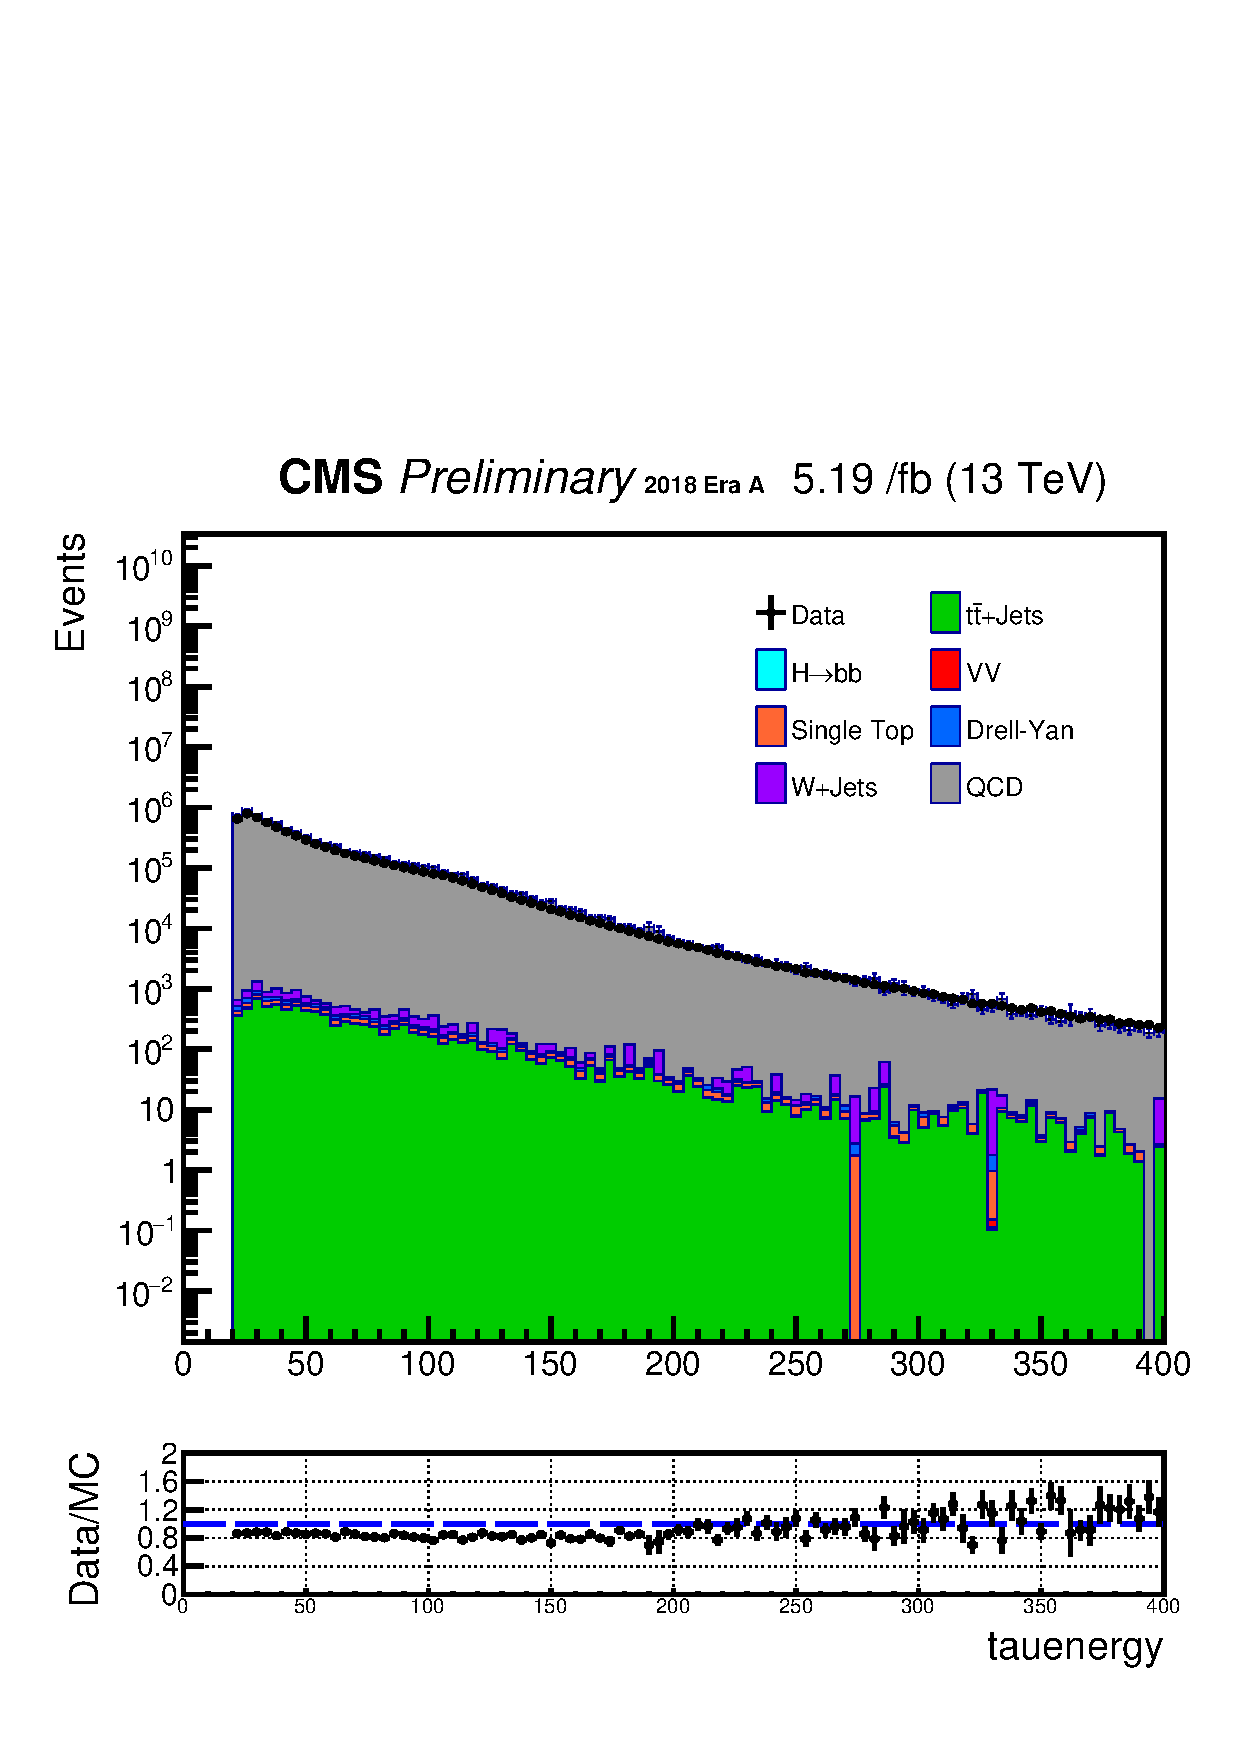
\includegraphics[width=0.47\linewidth]{figs/Data_log_AnalysisNote_MS-15_ctauS-10_tauenergy.pdf}
  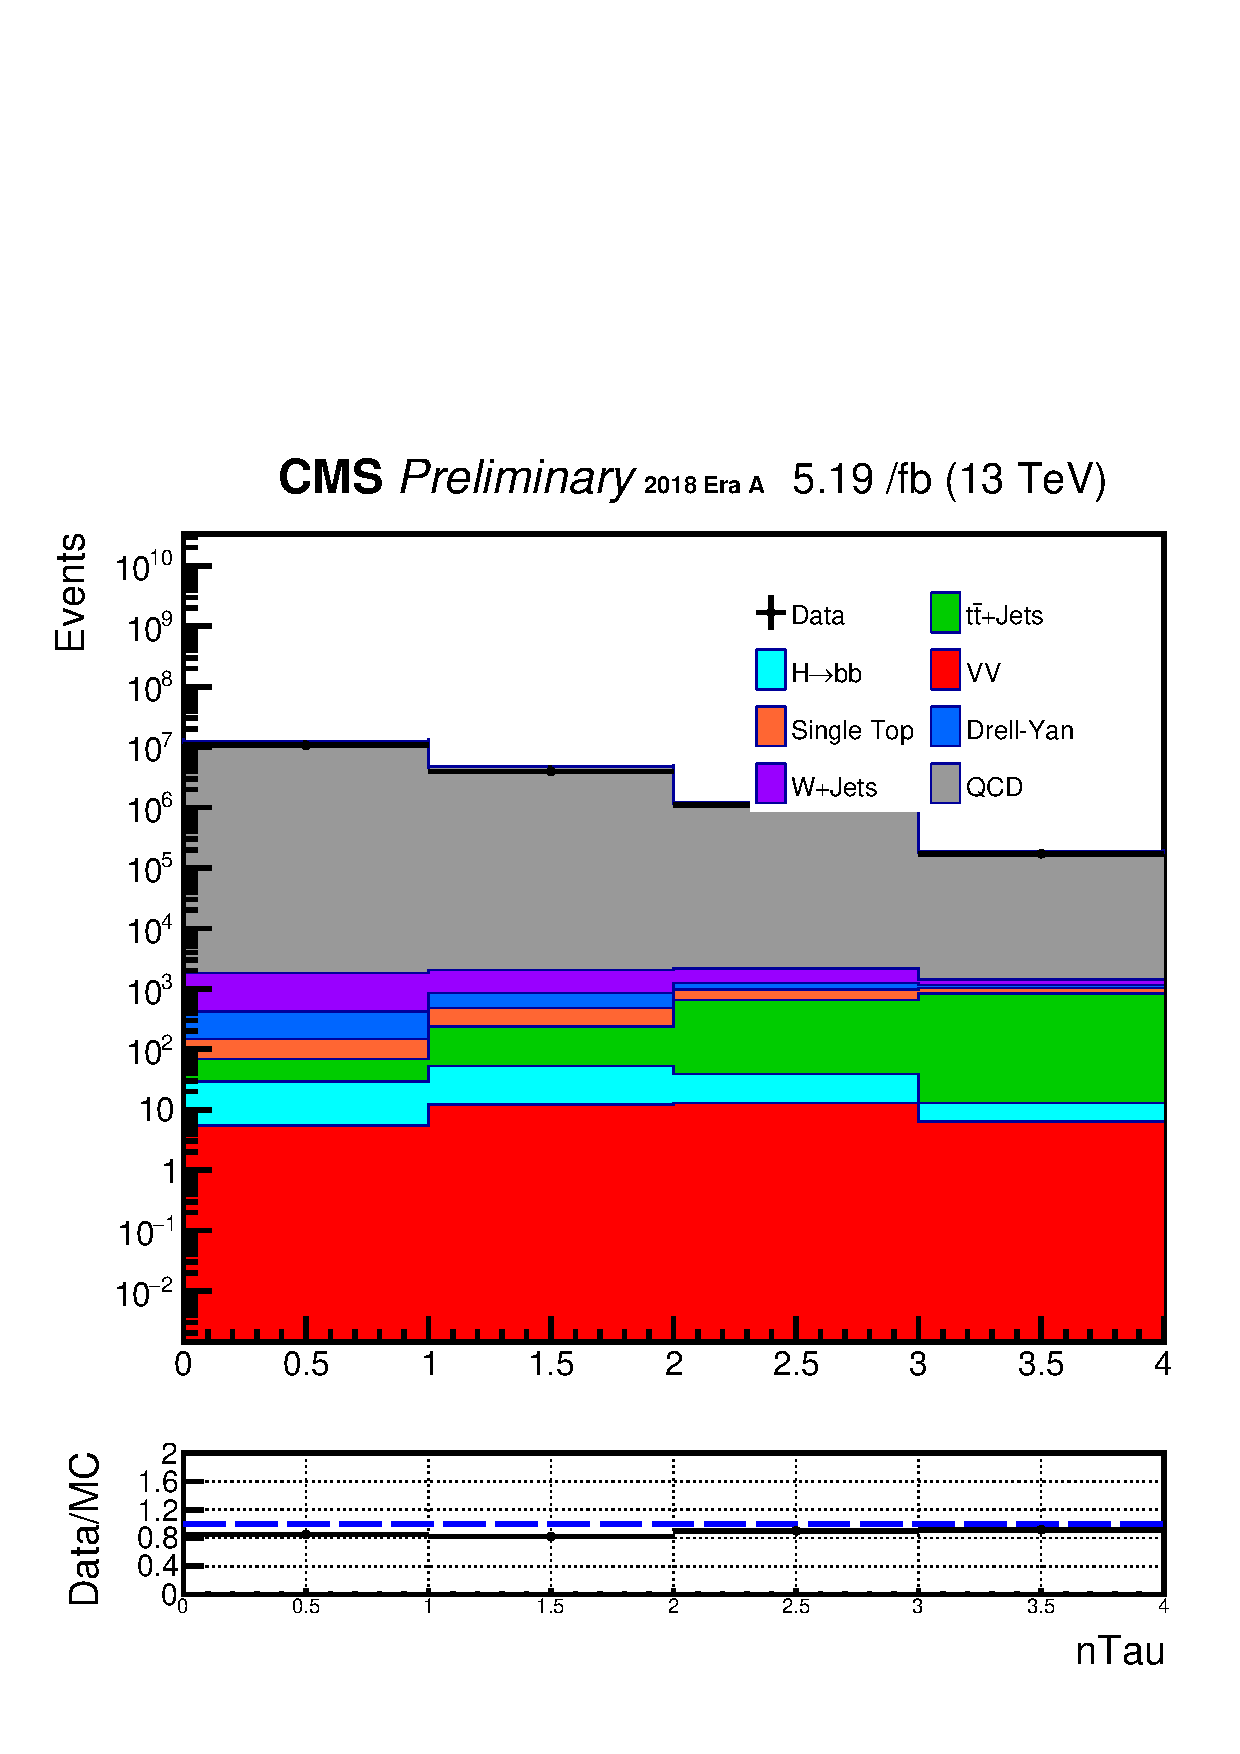
\includegraphics[width=0.47\linewidth]{figs/Data_log_AnalysisNote_MS-15_ctauS-10_nTau.pdf}
\end{figure}

\begin{figure}[h!]
  \caption{Data/MC of MET objects for pT, energy}
  \label{fig:METs}
  \centering
  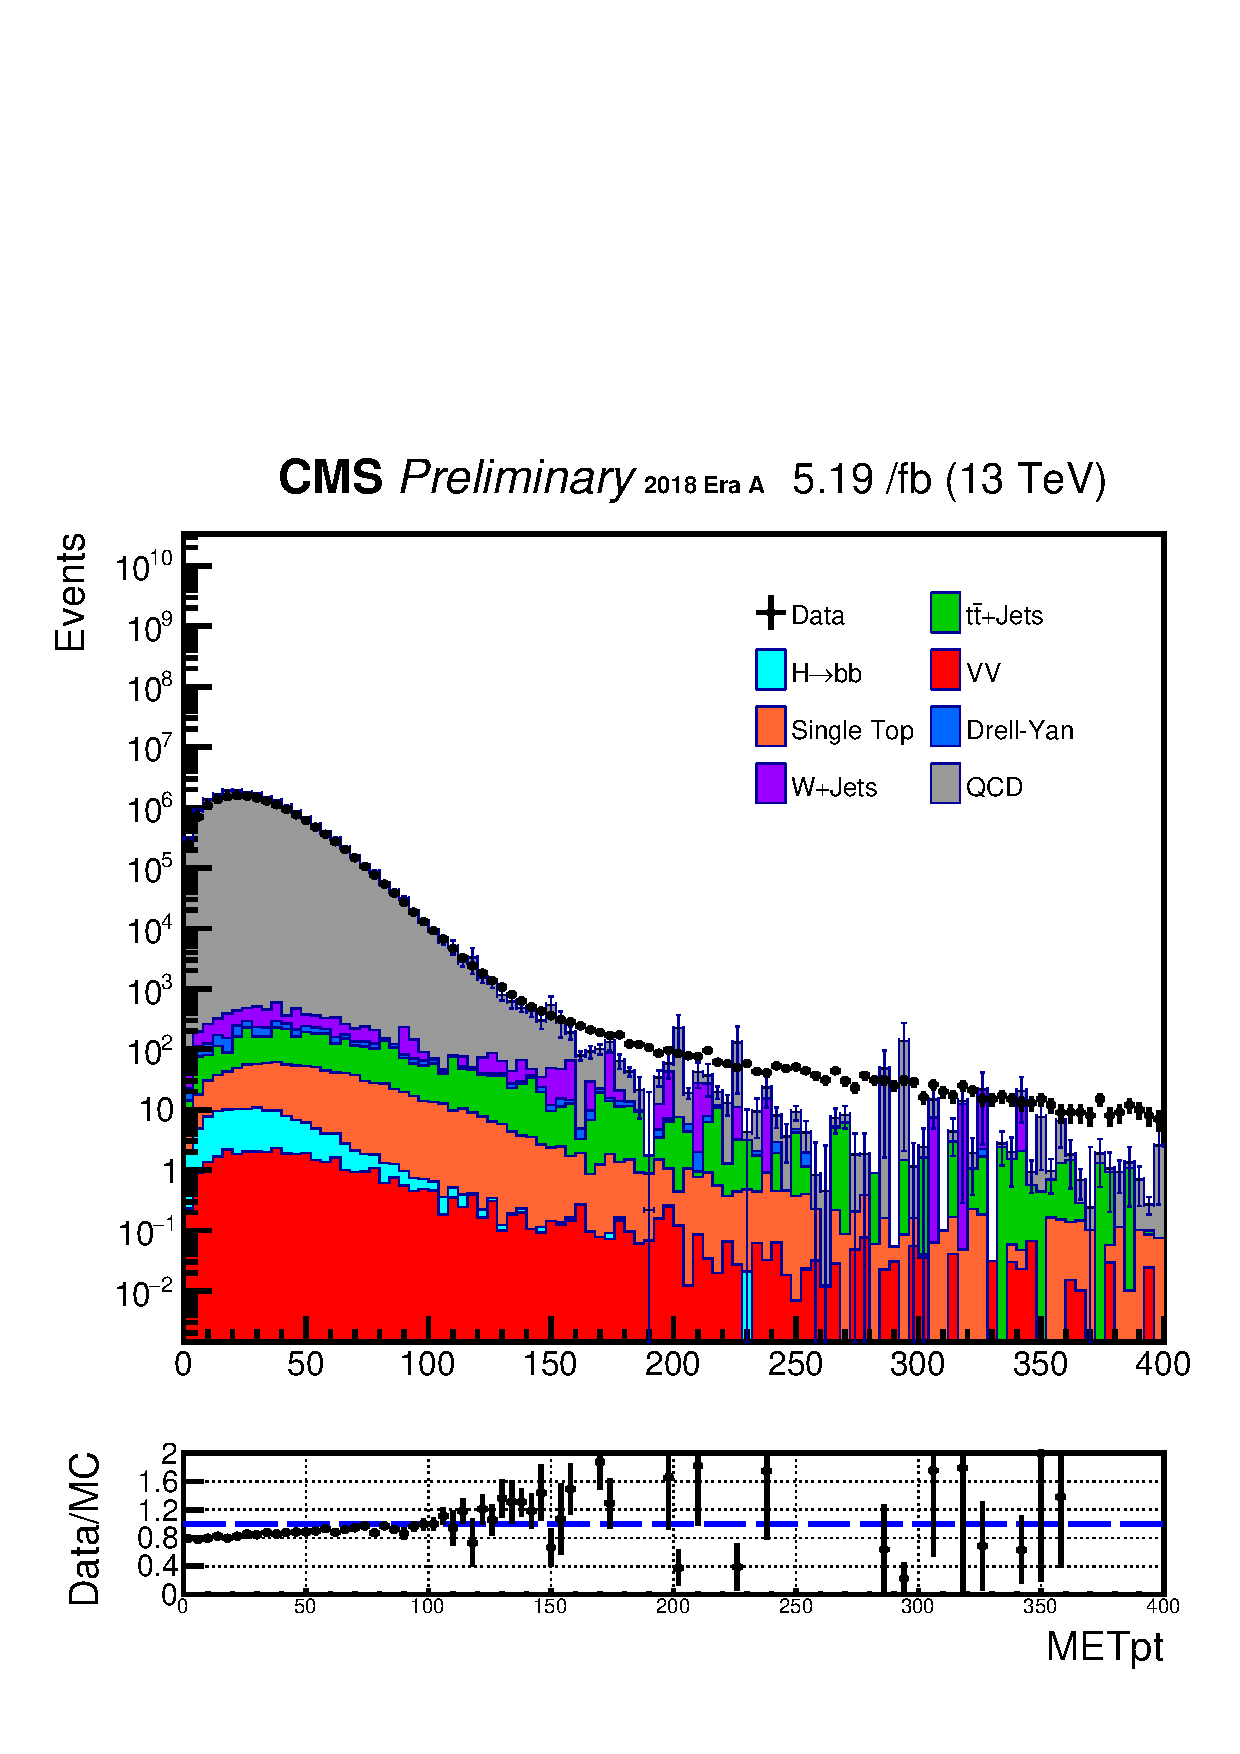
\includegraphics[width=0.47\linewidth]{figs/Data_log_AnalysisNote_MS-15_ctauS-10_METpt.pdf}
  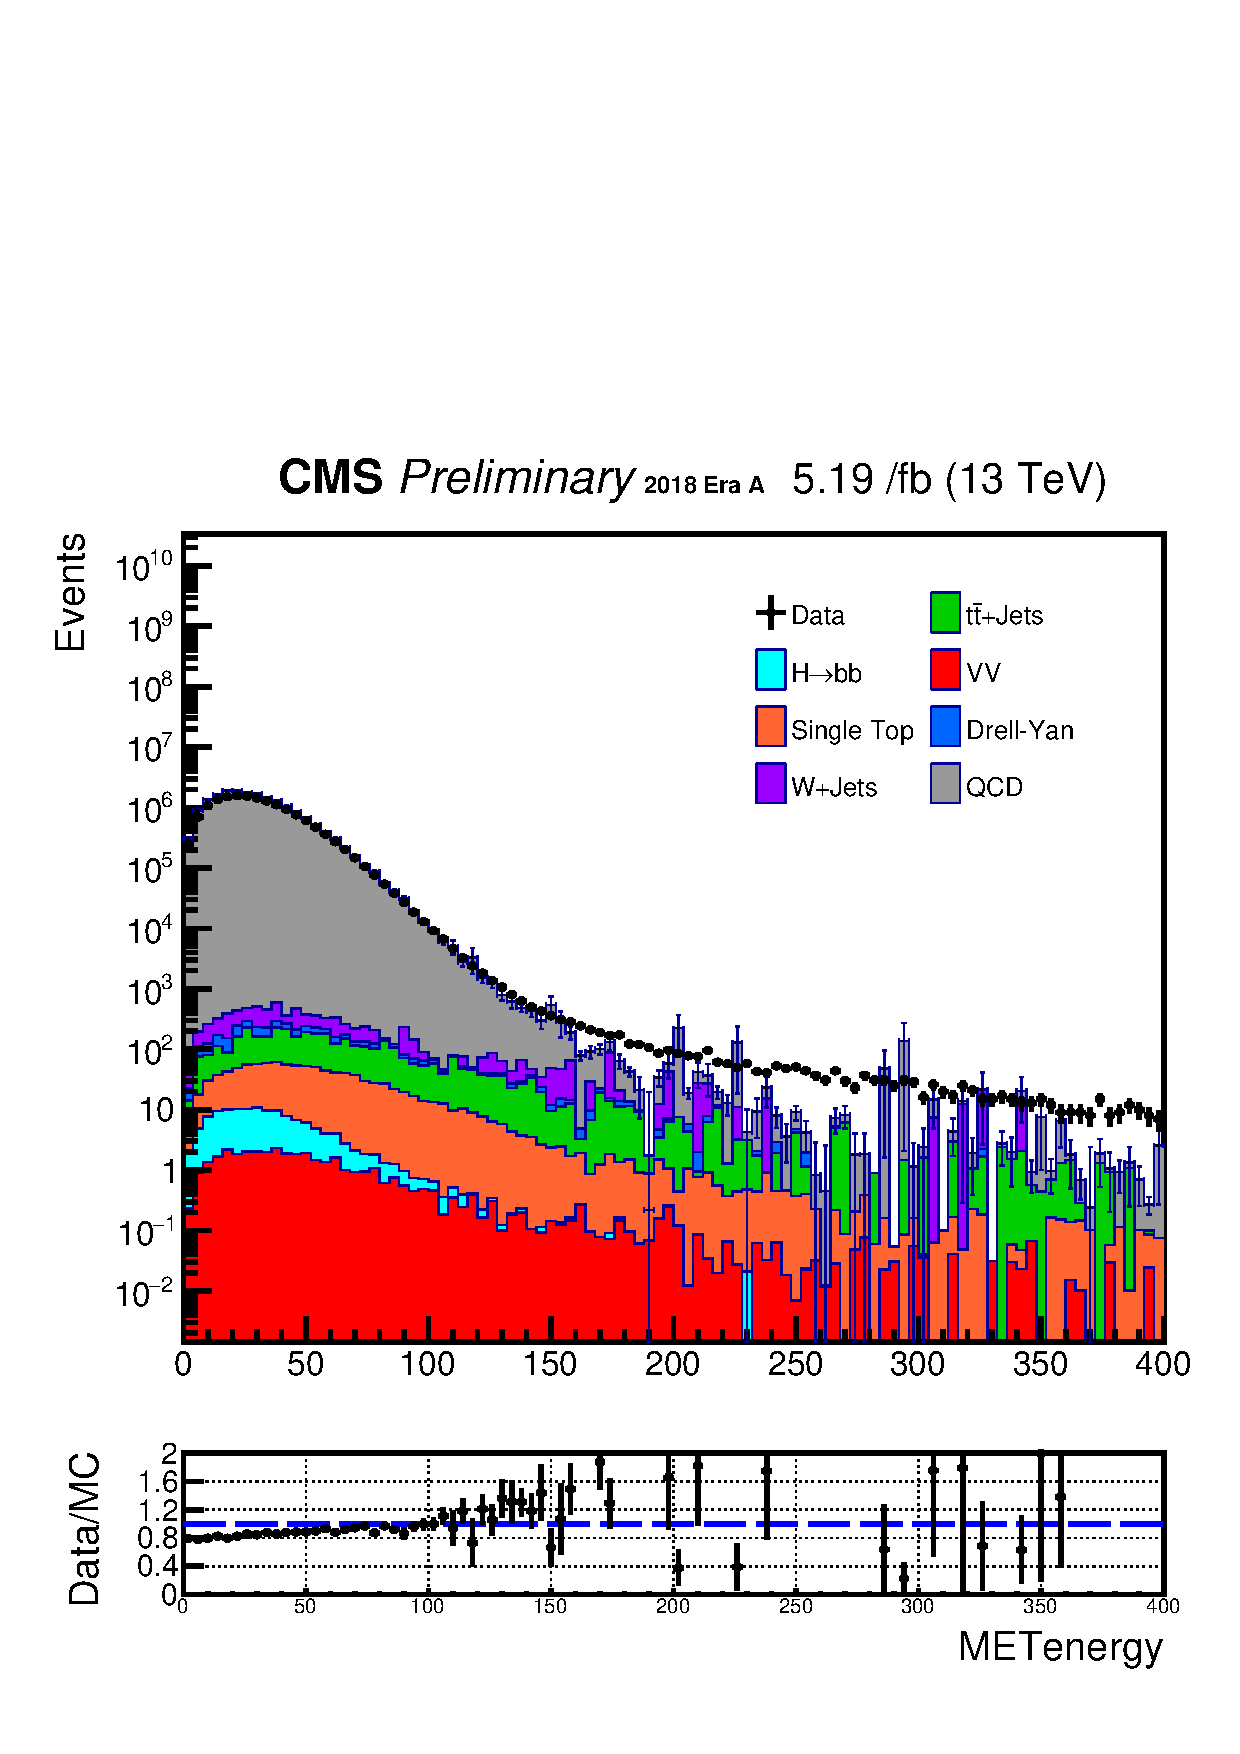
\includegraphics[width=0.47\linewidth]{figs/Data_log_AnalysisNote_MS-15_ctauS-10_METenergy.pdf}
\end{figure}




\section{Region of Interest}\label{sec:ROIs}
Tracks contain many essential qualities, such as the impact parameter significance and the four vectors.
LLP scalar particles decay in the tracker, so these track qualities should be good discriminant against the background.
However, we can not save all tracks in the event with all track information, as much as we have to filter out uninteresting events with the trigger system in CMS.
In our signal process, a geometrical concept can play a vital role in sorting out only relevant tracks for our analysis.
LLP scalar has no electric or color charge as described in section \ref{sec:theory}.
LLP scalar leaves no tracks in the tracker and decays into 2 charged tau leptons, which decay into at least one charged track ($\mu$, electron, at least one charged hadron).
Like in the pair production, two charged tracks often travel opposite directions.
Thus, a geometric convergence of 2 charged tracks should point to the decay vertex of the neutral LLP.
The tracker algorithm that we use to construct this ``Interesting Geometric Region'' provides us with a converged vertex, and the area around this vertex is referred to as the ``Region of Interest'' (ROI).
The complete reconstruction procedure of the Regions of Interest is detailed in the following subsections.
An ROI requires
\begin{itemize}
  \item Good quality track selection
  \item Vertex Fitted from pair-wise tracks by V0Fitter in CMSSW
  \item Cluster the fitted vertices to form a Region of Intrest (ROI)
  \item Look for tracks around $\Delta R=0.3$ around ROI to save its isolation information
\end{itemize}

\subsection{Tracks}\label{sec:ROI_tracks}

The analysis sources packedPFCandidates and lostTracks from MINIAOD.
Track parameters and convariance values will be propagated along the ROI production process and no value should be non-physical
\begin{itemize}
  \item !isinf(tracks.parameter)  and !isnan(tracks.parameter) 
  \item !isinf(tracks.covariance) and !isnan(tracks.covariance) 
  \item Number of valid hits $>$ 3
  \item pt $\geq$ 0.35
  \item Track $IPSig_{XY}\geq$2.
  \item Track $IPSig_{Z}\geq$-1.
  \item Track normalized $\chi^{2}\geq$10.
\end{itemize}


\subsection{Vertex Fitter}\label{sec:ROI_V0Fitter}

The analysis sources offlineBeamspot from MINIAOD for beamspot reference.
Vertex fitter is KalmanVertexFitter with vertex cuts as below.
\begin{itemize}
  \item Vertex $\chi^{2}\geq$6.63 
  \item Transverse Decay distance significance$\geq$15.
  \item V0mass $\geq$13000GeV
  \item cos($\theta_{XY}$) between x and p of V0 candidate $\geq$ 0
  \item cos($\theta_{XYZ}$) between x and p of V0 candidate $\geq$ -2
\end{itemize}
%New PVtight and opposite traveling track req

\subsection{ROI formation}\label{sec:ROI_ROIformation}
Fitted vertices are clustered to form a Region of Interest (ROI).
The clustering steps can be further detailed as below.
\begin{itemize}
  \item A fitted vertex is merged with another vertex if they are within 1cm. 
  \item A new ROI is formed where the position vector of ROI is averaged.
  \item Clustering is repeated until there is no other vertex within 1cm limit.
\end{itemize}
Although vertex clustering can be done with the step above, we can be creative and acquire more information.
Isolation, containing information about the ROI's environment, could also be helpful information.
We can obtain information about isolation by defining an isolation shell.
The shell's construction step is described below.
\begin{itemize}
  \item A cone of DeltaR < 0.3 around the center of the ROI is defined, where DeltaR is calculated with respect to the PV.
  \item A plane that is perpendicular to the axis of the cone and that contains the center of the ROI is the isolation plane. It becomes a circle. 
  \item Make the circle into a 3D sphere.
  \item Any tracks that pass through that sphere but not through the ROI are the annulus tracks.
\end{itemize}
With these essential tracks' information, we are ready to discriminate signals from the background.

\begin{figure}[h!]
  \centering
  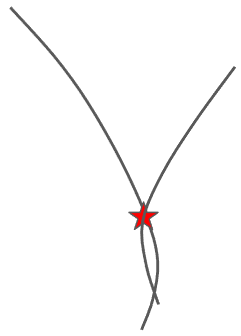
\includegraphics[width=0.27\linewidth]{figs/MLP3.png}
  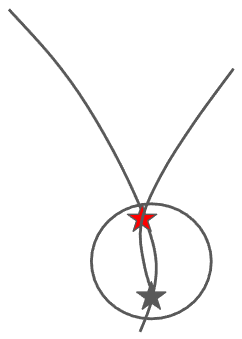
\includegraphics[width=0.27\linewidth]{figs/MLP2.png}
  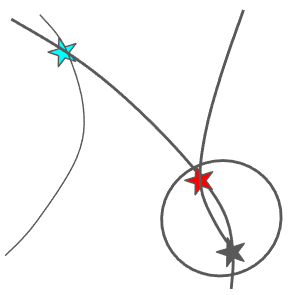
\includegraphics[width=0.27\linewidth]{figs/MLP1.png}
\caption{
        The figures display cartoons of the step-by-step formation of the Region of Interest (ROI).
        A dark line denotes a charged track: a muon track or electron track, or a charged hadron track from a tau lepton decay.
        The left figure shows the vertex (red star) fitted by KalmanVertexFitter in CMSSW from two charged tracks that decayed from a neutral LLP.
        The middle figure shows the clustering of the vertex, with the vertex (grey) formed by the extended tracks being clustered into the original ROI if the vertices are within a 1cm limit.
        The right figure shows the non-clustering of the vertex (sky) if the vertex is out of the 1cm limit. The track (thinner line), which forms a non-clustered vertex, is most likely from a pileup interaction.
	}
  \label{fig:Clustering}
\end{figure}

\begin{figure}[h!]
  \centering
  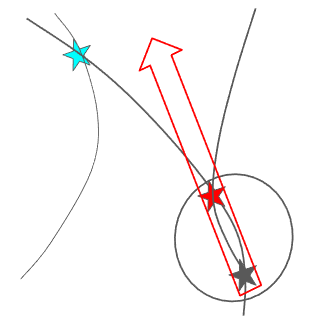
\includegraphics[width=0.4\linewidth]{figs/MLP4.png}
  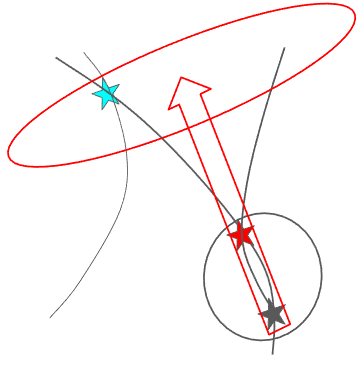
\includegraphics[width=0.4\linewidth]{figs/MLP5.png}
\caption{
        The figures display cartoons of the step-by-step formation of the shell structure.
        The left figure shows the axis of the cone when the axis goes through the center of ROI.
        The right figure shows the construction of the isolation plane, shown in the red color of the circle.
        The isolation plane has $\Delta$R=0.3.
        One can see the pileup track goes through the isolation plane in the cartoon.
        Thus, the shell formed by this isolation plane contains information about the isolation variable.
	}
  \label{fig:Clustering}
\end{figure}

\begin{figure}[h!]
  \caption{Data/MC of ROI distribution, distance along the transverse plane and beam direction}
  \label{fig:ROIs}
  \centering
  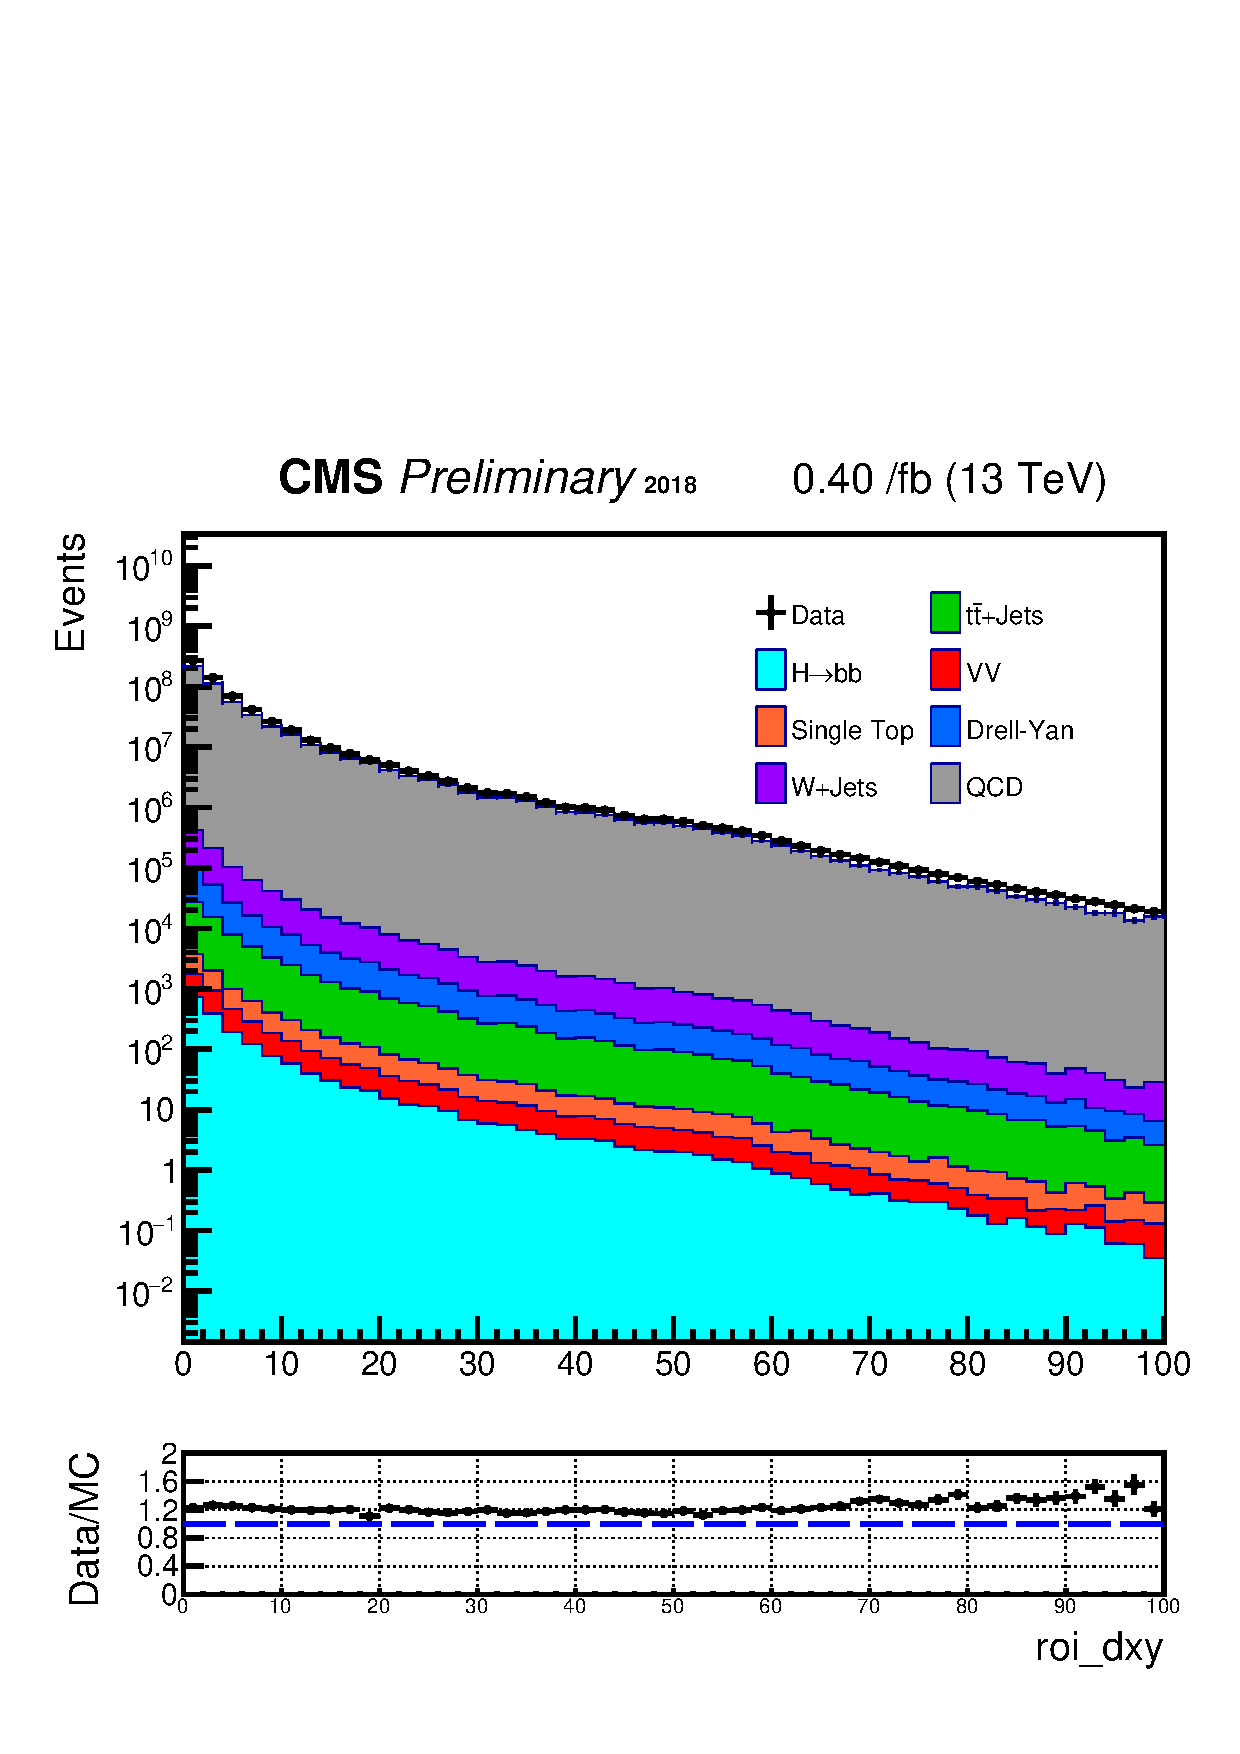
\includegraphics[width=0.47\linewidth]{figs/Data_AnalysisNoteplot_MS-15_ctauS-10_roi_dxy.pdf}
  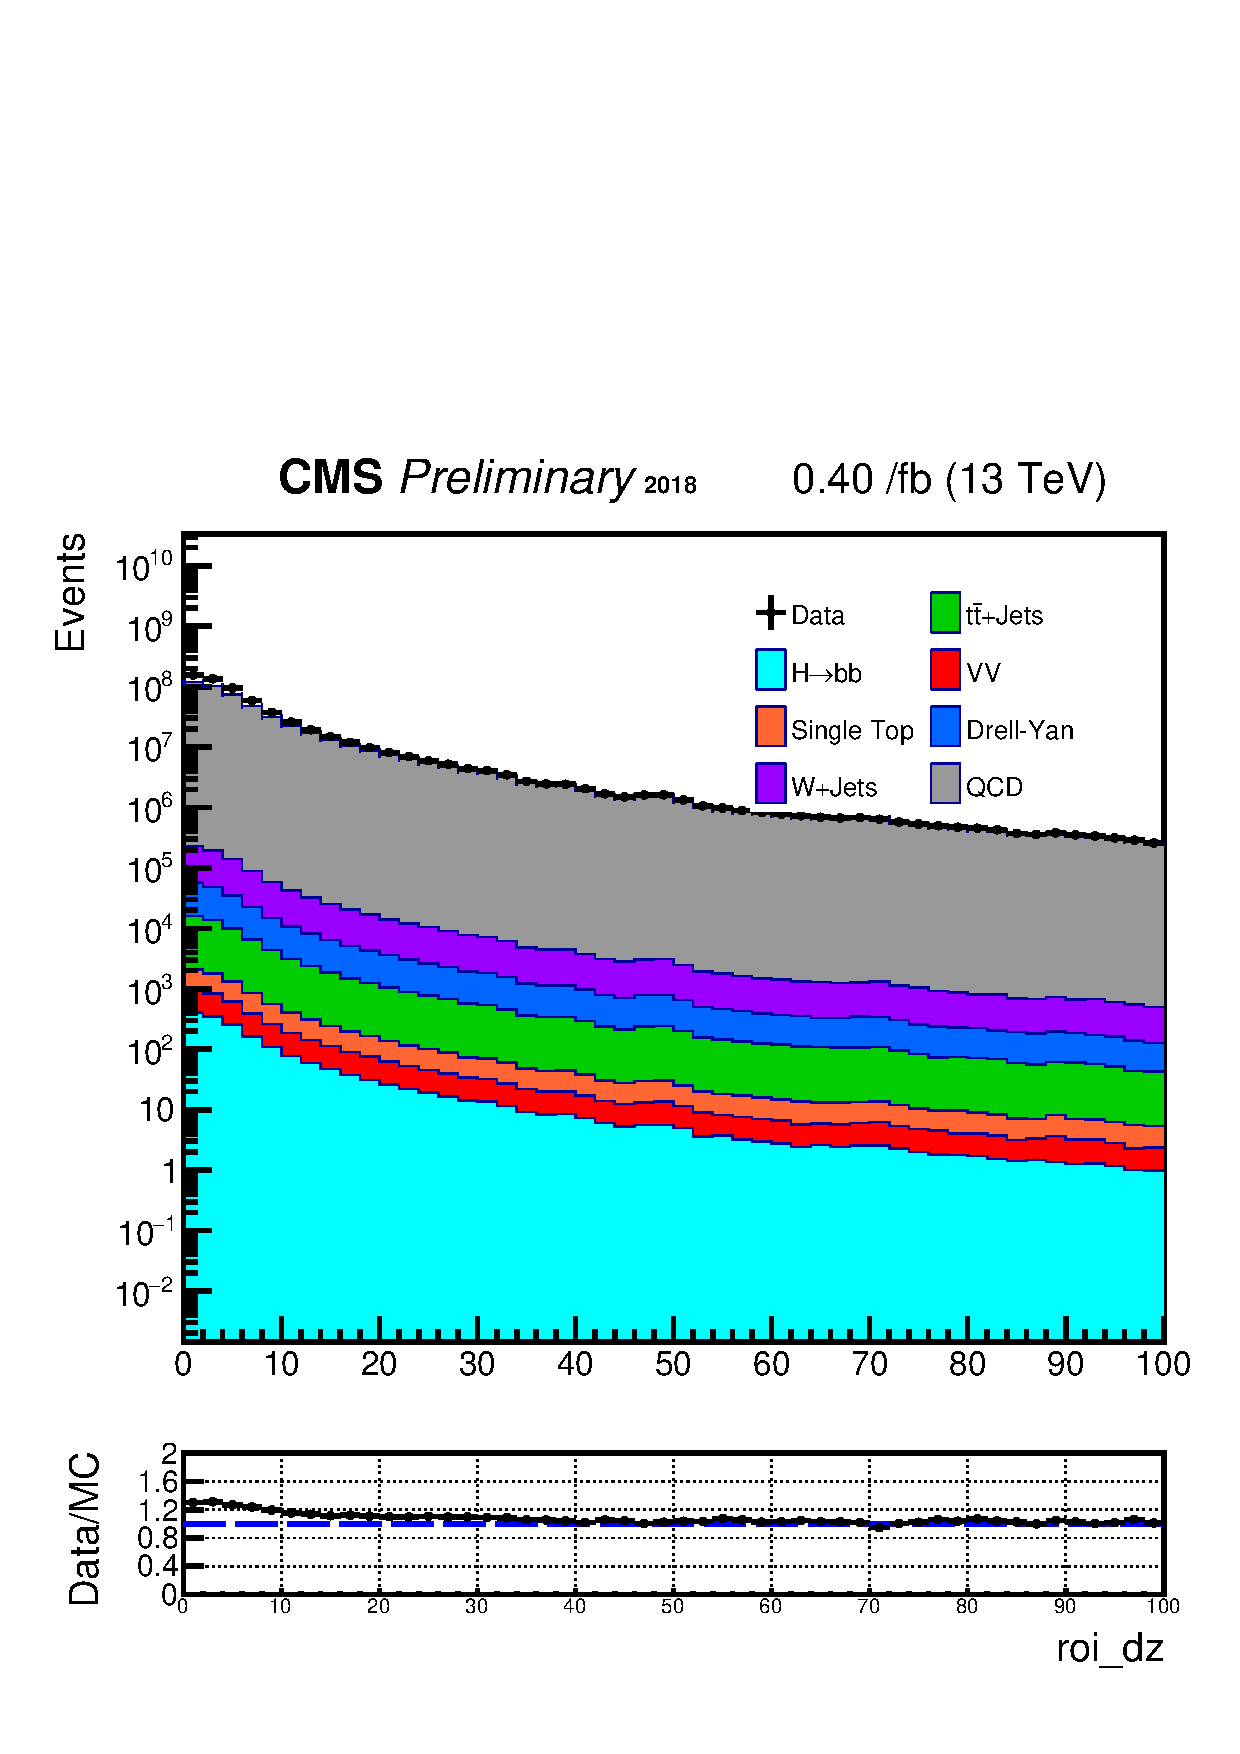
\includegraphics[width=0.47\linewidth]{figs/Data_AnalysisNoteplot_MS-15_ctauS-10_roi_dz.pdf}
\end{figure}

\begin{figure}[h!]
  \caption{Data/MC of ROI vertex and annulus track distribution}
  \label{fig:2ROIs}
  \centering
  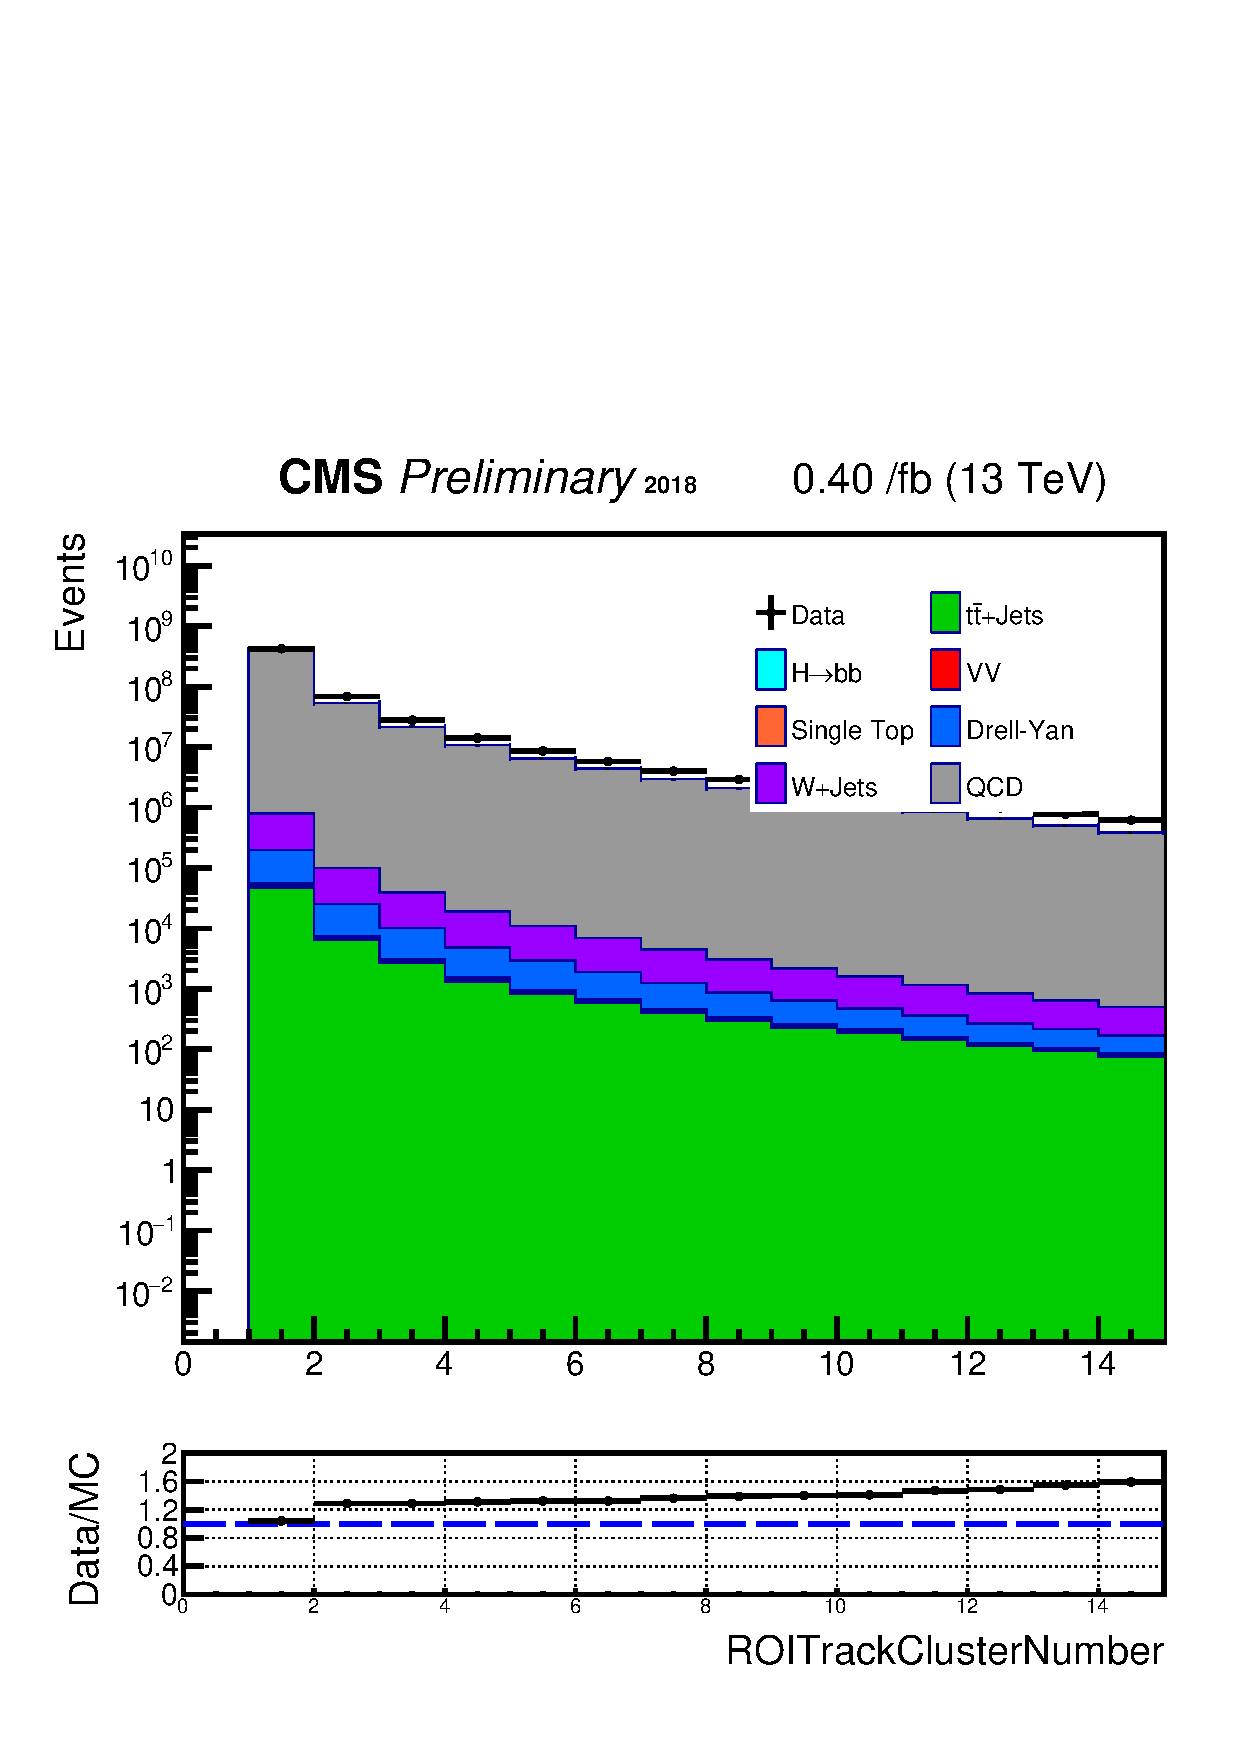
\includegraphics[width=0.47\linewidth]{figs/Data_AnalysisNoteplot_MS-15_ctauS-10_ROITrackClusterNumber.pdf}
  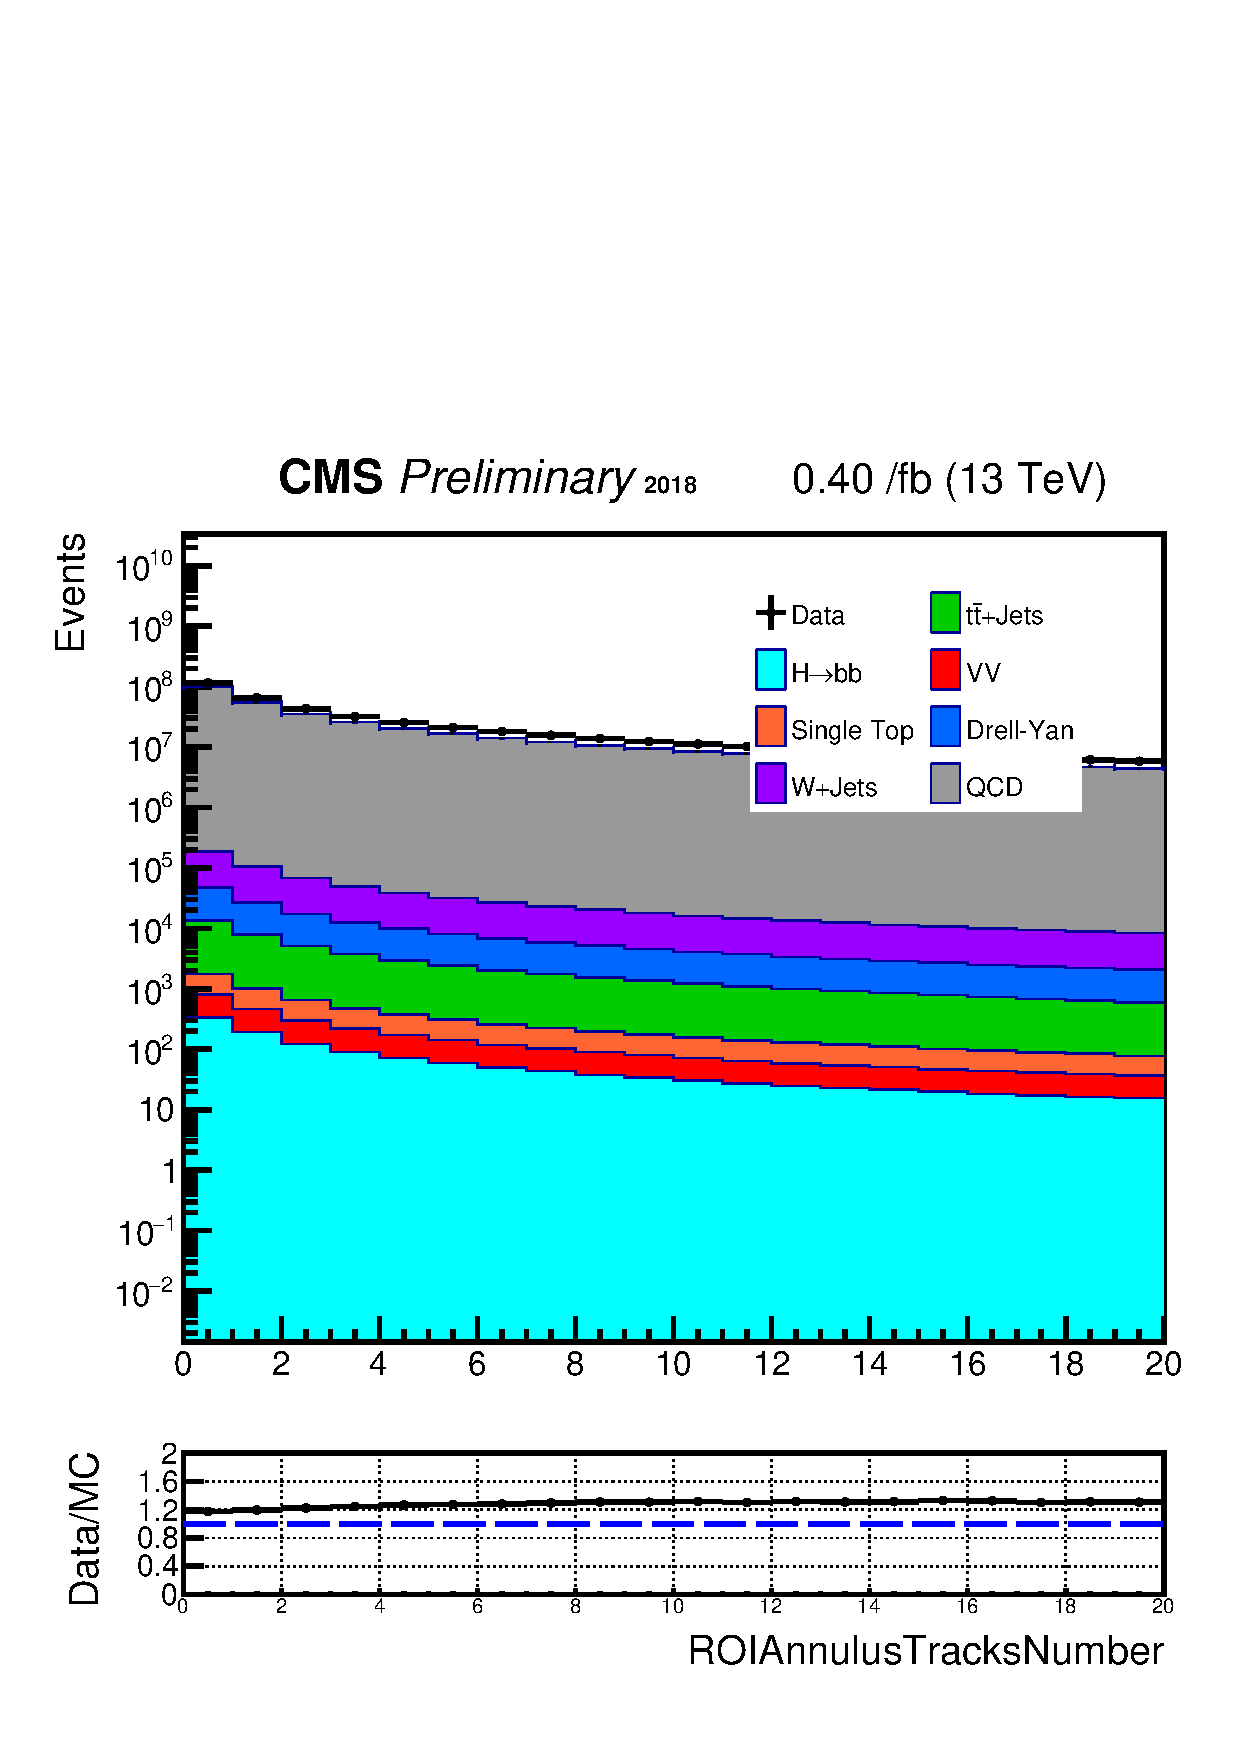
\includegraphics[width=0.47\linewidth]{figs/Data_AnalysisNoteplot_MS-15_ctauS-10_ROIAnnulusTracksNumber.pdf}
\end{figure}

\clearpage

\clearpage
\chapter{Machine Learning}\label{sec:machinelearning}
ROIs are artificial regions created by the CMSSW mechanism, displaced vertex candidates.
ROIs contain thorough information about fitted tracks, vertices, and isolation, following the formation procedure described in the previous section.
The exhaustive variables saved in each ROI contain information that directly and indirectly tells whether the ROI is from the signal or background process.
Given the extensive amount of variables within ROIs, it is inappropriate to use ROIs' single or a few variables as our tagging variables, like in ZH analysis ~\cite{ZHAN}.
It is also inefficient to implement a cut-based approach due to having so many variables from ROI.
The optimization process for all these vertex, isolation, and track variables would be extremely time-consuming, inefficient, and error-prone.
Therefore, the analysis exploits machine learning (ML) for this multivariate analysis.
Boosted decision trees will also face a similar problem as cut-based analysis.
Deep Neural Networks are the most adaptable ML algorithm for this analysis method, in which the algorithm inputs an extensive list of ROI variables into a neural network and receives a final score to discriminate ROIs that arise in signal process versus background processes.
The list of variables inputted into the ML algorithms is provided in subsection \ref{sec:MLIV}.

The analysis uses Keras-Tensorflow for its ML platform.
CMSSW includes Keras-Tensorflow, which enables simple and easy usage of Keras-Tensorflow with simple commands in various CMS remote clusters.
For CMSSW\_10\_6\_12 (to have access to the B Parking trigger path), the Keras-Tensorflow version is 2.3.1.
It runs with CPUs and GPUs.
\section{Machine Learning Input Variables}\label{sec:MLIV}
As discussed in chapter \ref{sec:objects}, the ROI has vertex and shell (isolation) information.
Vertex information is trained with 27 different variables, which are listed and categorized in Tables ~\ref{tab:ROITCvars}.
%, ~\ref{tab:ROIANvars}, and ~\ref{tab:ROIEVvars}.

\begin{table}[htb]
\caption{ROI (trackCluster) variables by category}
\begin{center}
\begin{tabular}{r|l|l}\hline
 TrackCluster & Position & TrackClusters.vx() - primaryVertex.X() \\
              & Position & TrackClusters.vy() - primaryVertex.Y() \\
              & Position & TrackClusters.vz() - primaryVertex.Z() \\
              & Covariance & TrackClusters.vertexCovariance()(0,0) \\
              & Covariance & TrackClusters.vertexCovariance()(0,1) \\
              & Covariance & TrackClusters.vertexCovariance()(0,2) \\
              & Covariance & TrackClusters.vertexCovariance()(1,0) \\
              & Covariance & TrackClusters.vertexCovariance()(1,1) \\
              & Covariance & TrackClusters.vertexCovariance()(1,2) \\
              & Track0,1 & Track0,1.pt \\
              & Track0,1 & Track0,1.eta \\
              & Track0,1 & Track0,1.phi \\
              & Track0,1 & Track0,1.dxy \\
              & Track0,1 & Track0,1.dz \\
              & Track0,1 & Track0,1.dxyError \\
              & Track0,1 & Track0,1.dzError \\
              & Track0,1 & Track0,1.normalizedChi2 \\
              & Track0,1 & Track0,1.HighPurityInt \\
 \hline
 \hline
\end{tabular}
\label{tab:ROITCvars}
\end{center}
\end{table}



Shell information is trained with 9 different variables, which are listed in Tables ~\ref{tab:ROIANvars}.

\begin{table}[htb]
\caption{ROI (Annulus) variables by category}
\begin{center}
\begin{tabular}{r|l|l}\hline
 Annulus      & pfCandidate/LostTracks & pfCandidate/LostTracks.pt \\
              & pfCandidate/LostTracks & pfCandidate/LostTracks.eta \\
              & pfCandidate/LostTracks & pfCandidate/LostTracks.phi \\
              & pfCandidate/LostTracks & pfCandidate/LostTracks.dxy \\
              & pfCandidate/LostTracks & pfCandidate/LostTracks.dz \\
              & pfCandidate/LostTracks & pfCandidate/LostTracks.dxyError \\
              & pfCandidate/LostTracks & pfCandidate/LostTracks.dzError \\
              & pfCandidate/LostTracks & pfCandidate/LostTracks.normalizedChi2 \\
              & pfCandidate/LostTracks & pfCandidate/LostTracks.HighPurityInt \\
 \hline
 \hline
\end{tabular}
\label{tab:ROIANvars}
\end{center}
\end{table}

We input vertex and shell information into separate ML networks. Thus, we get two final products from the ML networks, one for the vertex information and the other for the shell information.

 \begin{figure}[h!]
   \label{fig:NetworkML}
   \centering
   \includegraphics[width=0.6\linewidth]{figs/PhiVNet.png}
   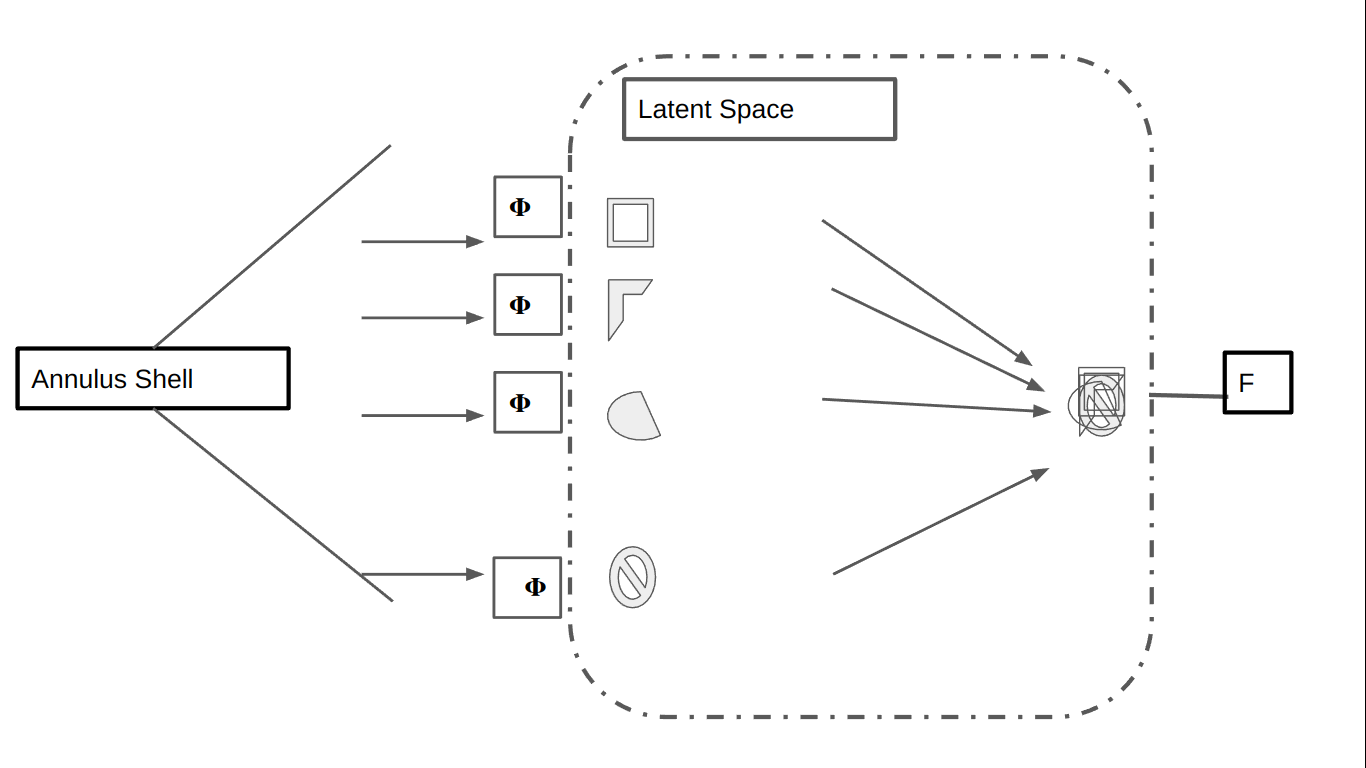
\includegraphics[width=0.6\linewidth]{figs/PhiANet.png}
   \caption{Simple cartoon showing ML network for vertex and annulus shell.}
 \end{figure}

%\begin{table}[htb]
%\caption{Event variables by category}
%\begin{center}
%\begin{tabular}{r|l|l}\hline
%  ROI    & Position & x \\
%         & Position & y \\
%         & Position & z \\
% \hline
% \hline
%\end{tabular}
%\label{tab:ROIEVvars}
%\end{center}
%\end{table}

\section{Fine-Tuning of ML environemnt}
CMSSW includes an image container for Keras-Tensorflow, and researchers can also submit remote batch jobs for its ML training.
The analysis tested multiple variables (such as epoch numbers, batch sizes, phi sizes, and f sizes) of our DNN layers thanks to the submission of remote batch jobs with CMSSW's Keras-Tensorflow image container.
The analysis tested different signal vs. background dataset combinations for maximum discriminant power.
The list of mass scale and lifetime tested for signal points are listed in the appendix \ref{sec:train}.
Different SM physics process (and their compositions) tested for background process are also listed in the appendix \ref{sec:train}.

The final Tensorflow product used for the analysis was trained with parameters in table \ref{tab:ROIParam}.
Keras-Tensorflow DNN variable information was fine-tuned with these variables for the maximum Area Under the Curve (AUC) value.
Its information is listed in the table \ref{tab:ROIParam}.
\begin{table}[htb]
\caption{Parameters for ML network}
\begin{center}
\begin{tabular}{r|l}\hline
Epoch & 300 \\
batch size & 250 \\
Phi sizes & (64,128,256) for vertex ,(32,64,128) for shell \\
f sizes & (256,128,32) \\
Signal & ggHSSTo4Tau-MS15GeV-c$\tau$100mm  \\
Background & QCD\_Pt120-170\_MuEneriched and TTJets \\
 \hline
 \hline
\end{tabular}
\label{tab:ROIParam}
\end{center}
\end{table}


\section{ML scores of the ROIs}
More than 10 ROIs per event often exist from our ROI reconstruction mechanism.
However, we do not need all ROIs per event, as many of them are low-scoring ROIs that come from track misconstruction and others.
The signal process has two scalar decays as in Figure~\ref{fig:feynmanggH}, and it is reasonable to use only the two highest-scoring ROIs for our analysis.
Thus, we define the leading ROI (leadROI) as an ROI with the highest vertex score in the event.
Likewise, it would be easy to define the subleading ROI (subleadROI) as an ROI with the second highest vertex score in the event.
However, the subleadROI is not simply the second highest-scoring ROI of the event due to the non-negligible lifetime of $\tau$ leptons in the detector.
After obtaining an ROI with the highest ML vertex score, we search for the next highest scored ROI, $\Delta\Phi>$0.4, from the leading ROI to avoid counting ROI from the same LLP decay.
The ordering is done by vertex discriminant since it is more potent than the shell discriminant.
For better numerical representation, we use log base 10 value of ROI vertex score subtracted from 1.
Mathmatical definition of loglead and logexclead are in formulae \ref{eq:log} and \ref{eq:logexc}. 
\begin{equation}
\label{eq:log}
	loglead = Log10(1-ROI's\;leading\;Vertex\;score)
\end{equation}
\begin{equation}
\label{eq:logexc}
	logexclead = Log10(1-ROI's\;subleading\;Vertex\;score),\;with\;\Delta\Phi(lead,sublead) \geq 0.4.
\end{equation}
%More detailed explanations are described in section~\ref{sec:lifetimeROI}.)  
%The cuts on the leading ROI, and the subleading ROI are optimized based on maximizing the punzi significance formula with value $\sigma$ set to discovery value of 5.  
%\begin{equation}\label{eq:significance}
%    \sigma(N_{\mathrm{displaced-tag}}) = \frac{S(N_{\mathrm{displaced-tag}})} {\sqrt{B(N_{\mathrm{displaced-tag}})} + 2.5 }.
%\end{equation}

%\begin{figure}[h!]
%  \caption{Tensorflow scores}
%  \label{fig:TensorFlow scores}
%  \centering
%  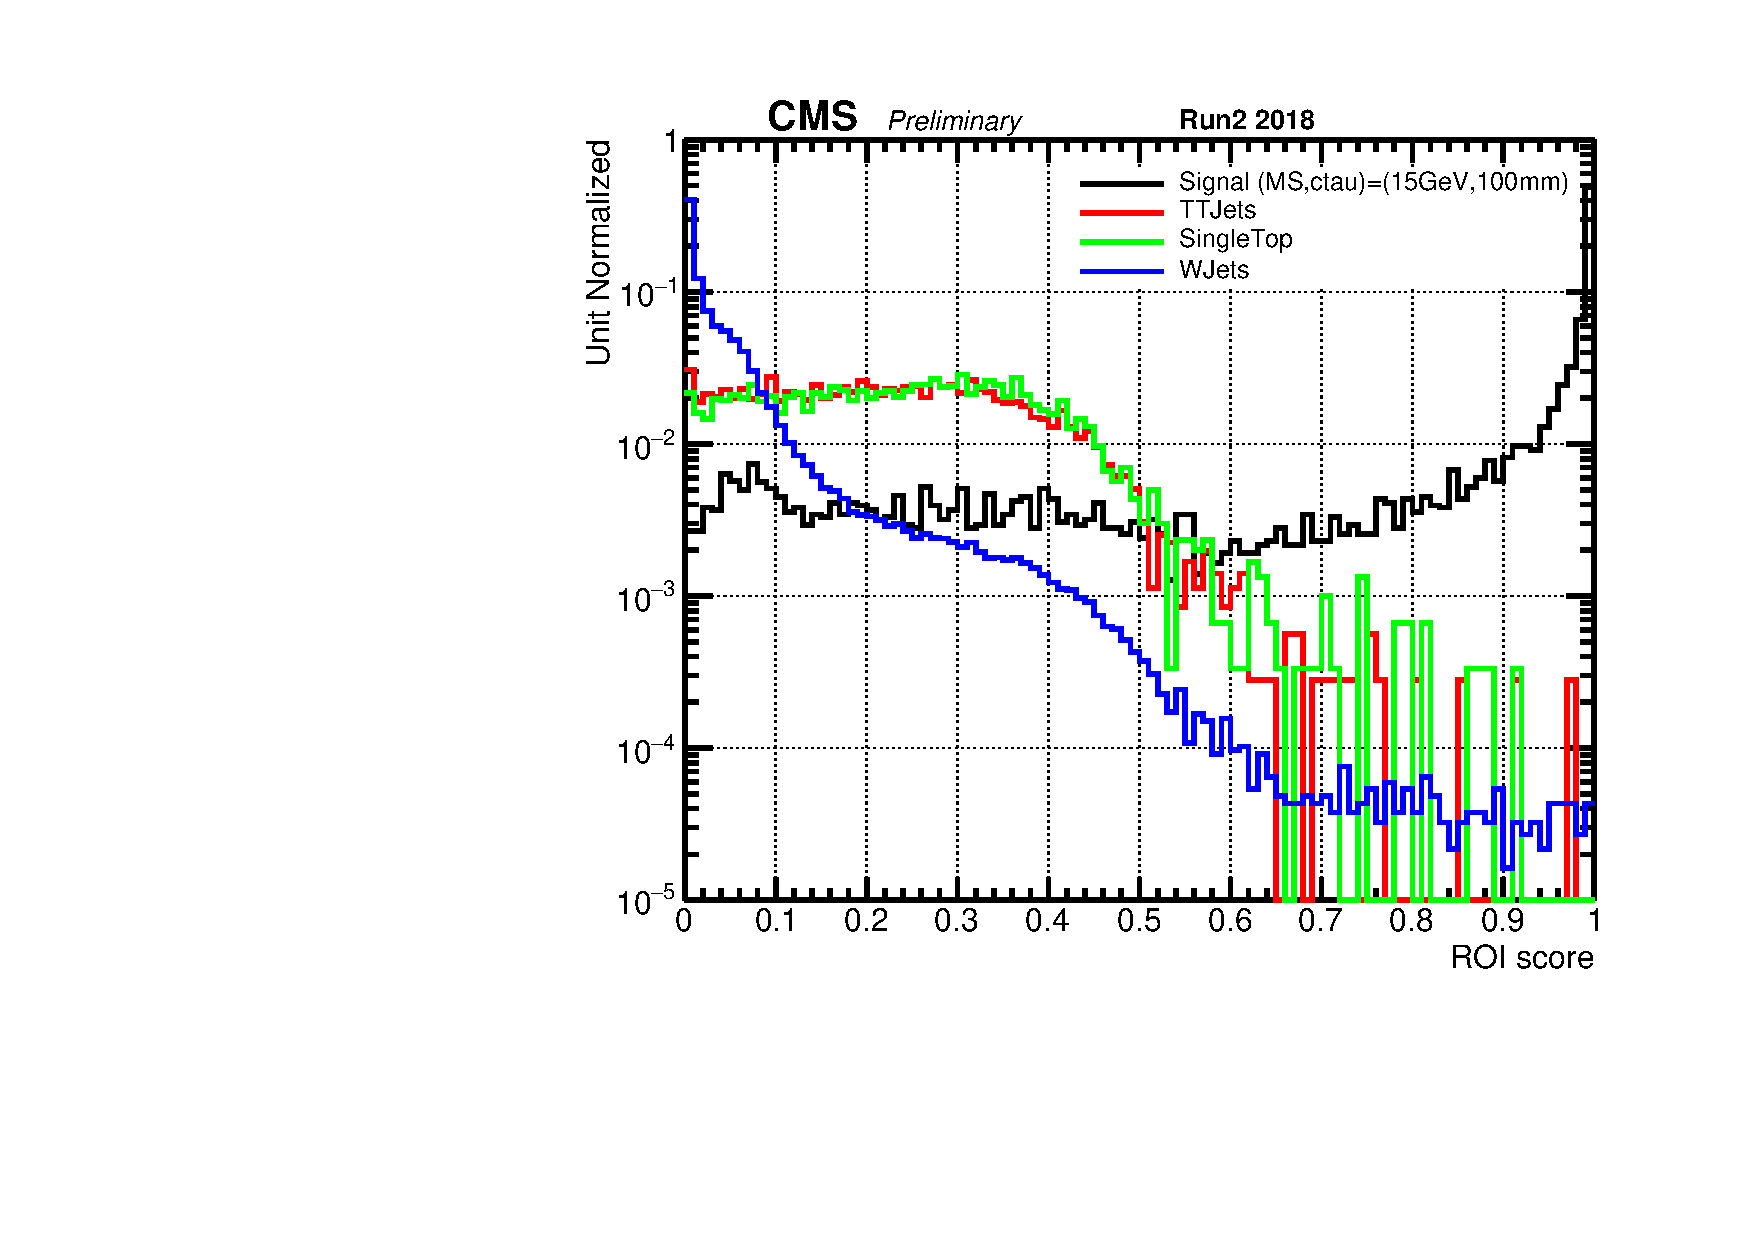
\includegraphics[width=0.67\linewidth]{figs/Tensorflow_Disc_mostrecent.pdf}
%
%\end{figure}

 \begin{figure}[h!]
   \label{fig:leadROIscore}
   \centering
   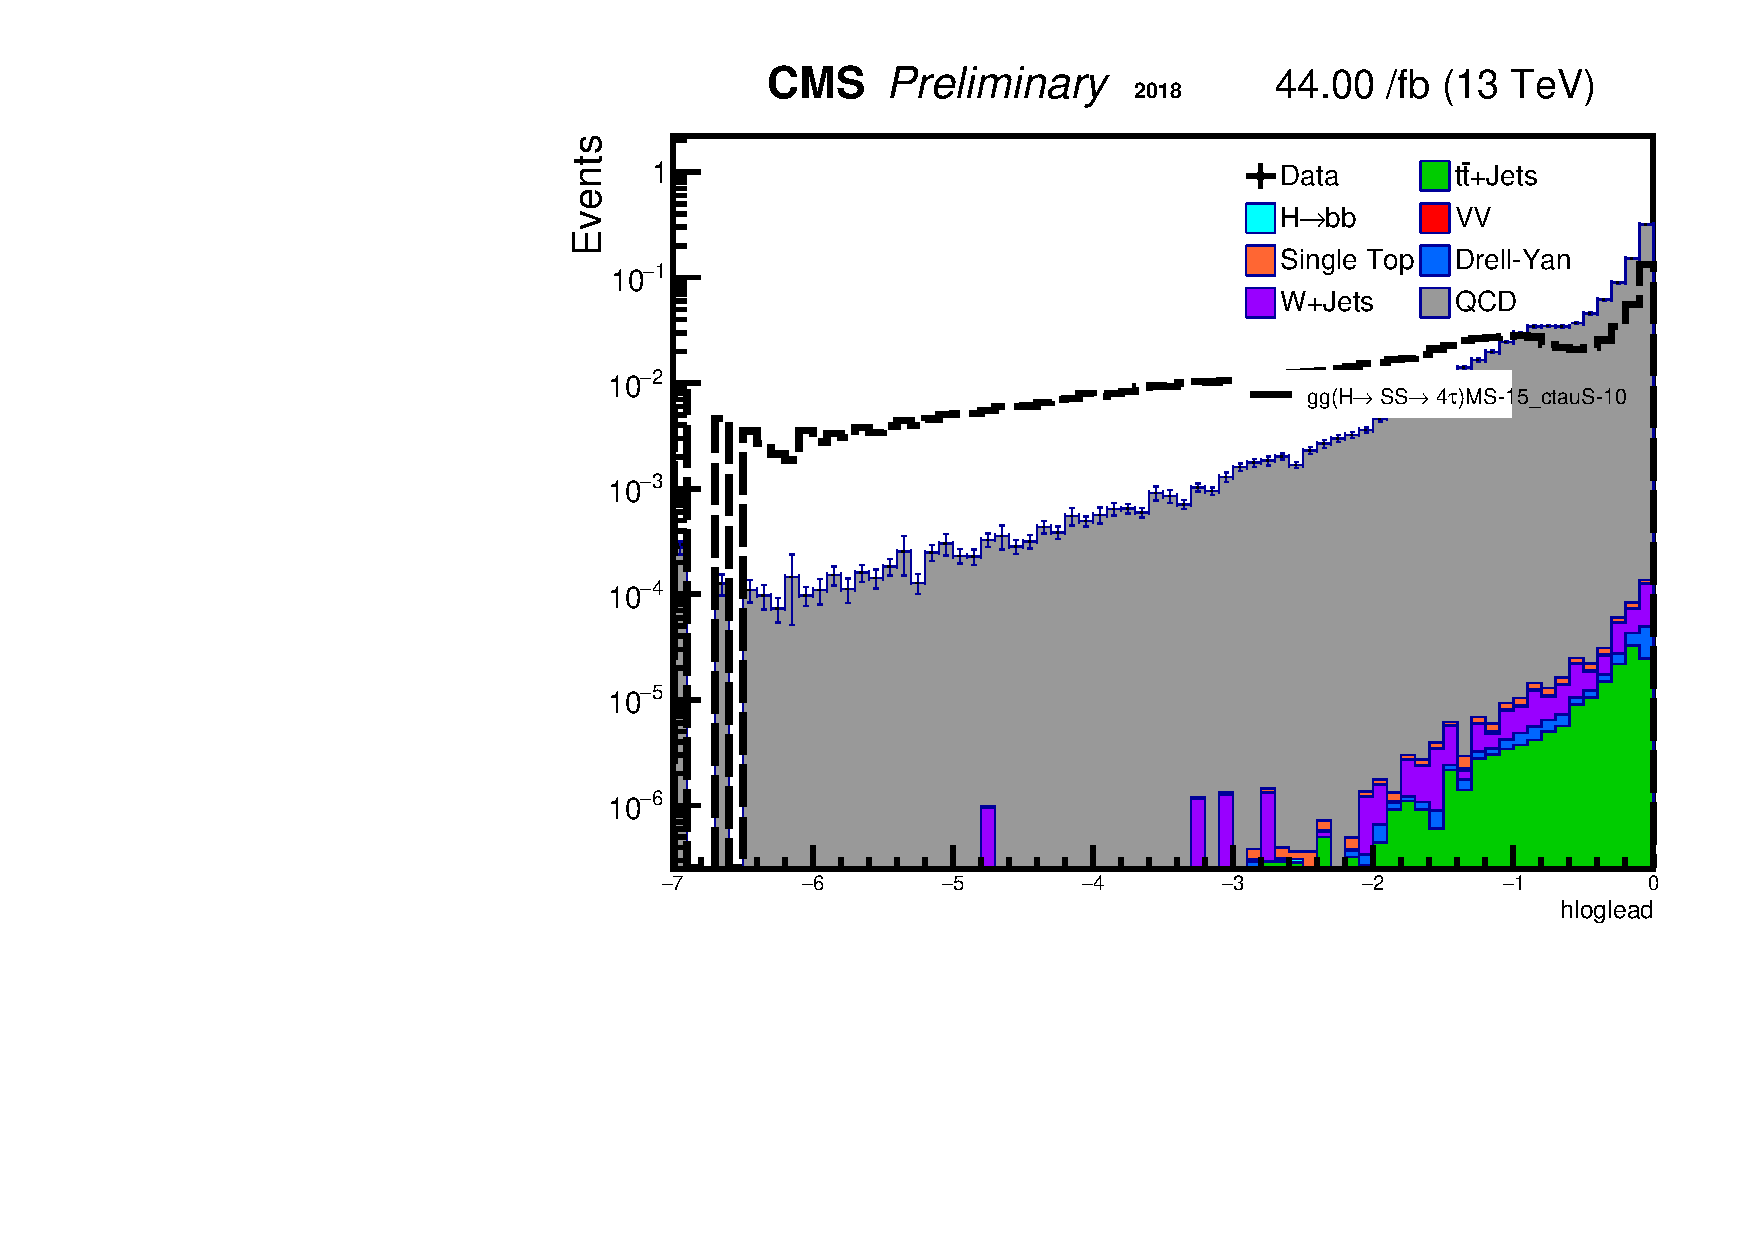
\includegraphics[width=0.47\linewidth]{figs/log_Oct6ANVars_MS-15_ctauS-10_hloglead.pdf}
   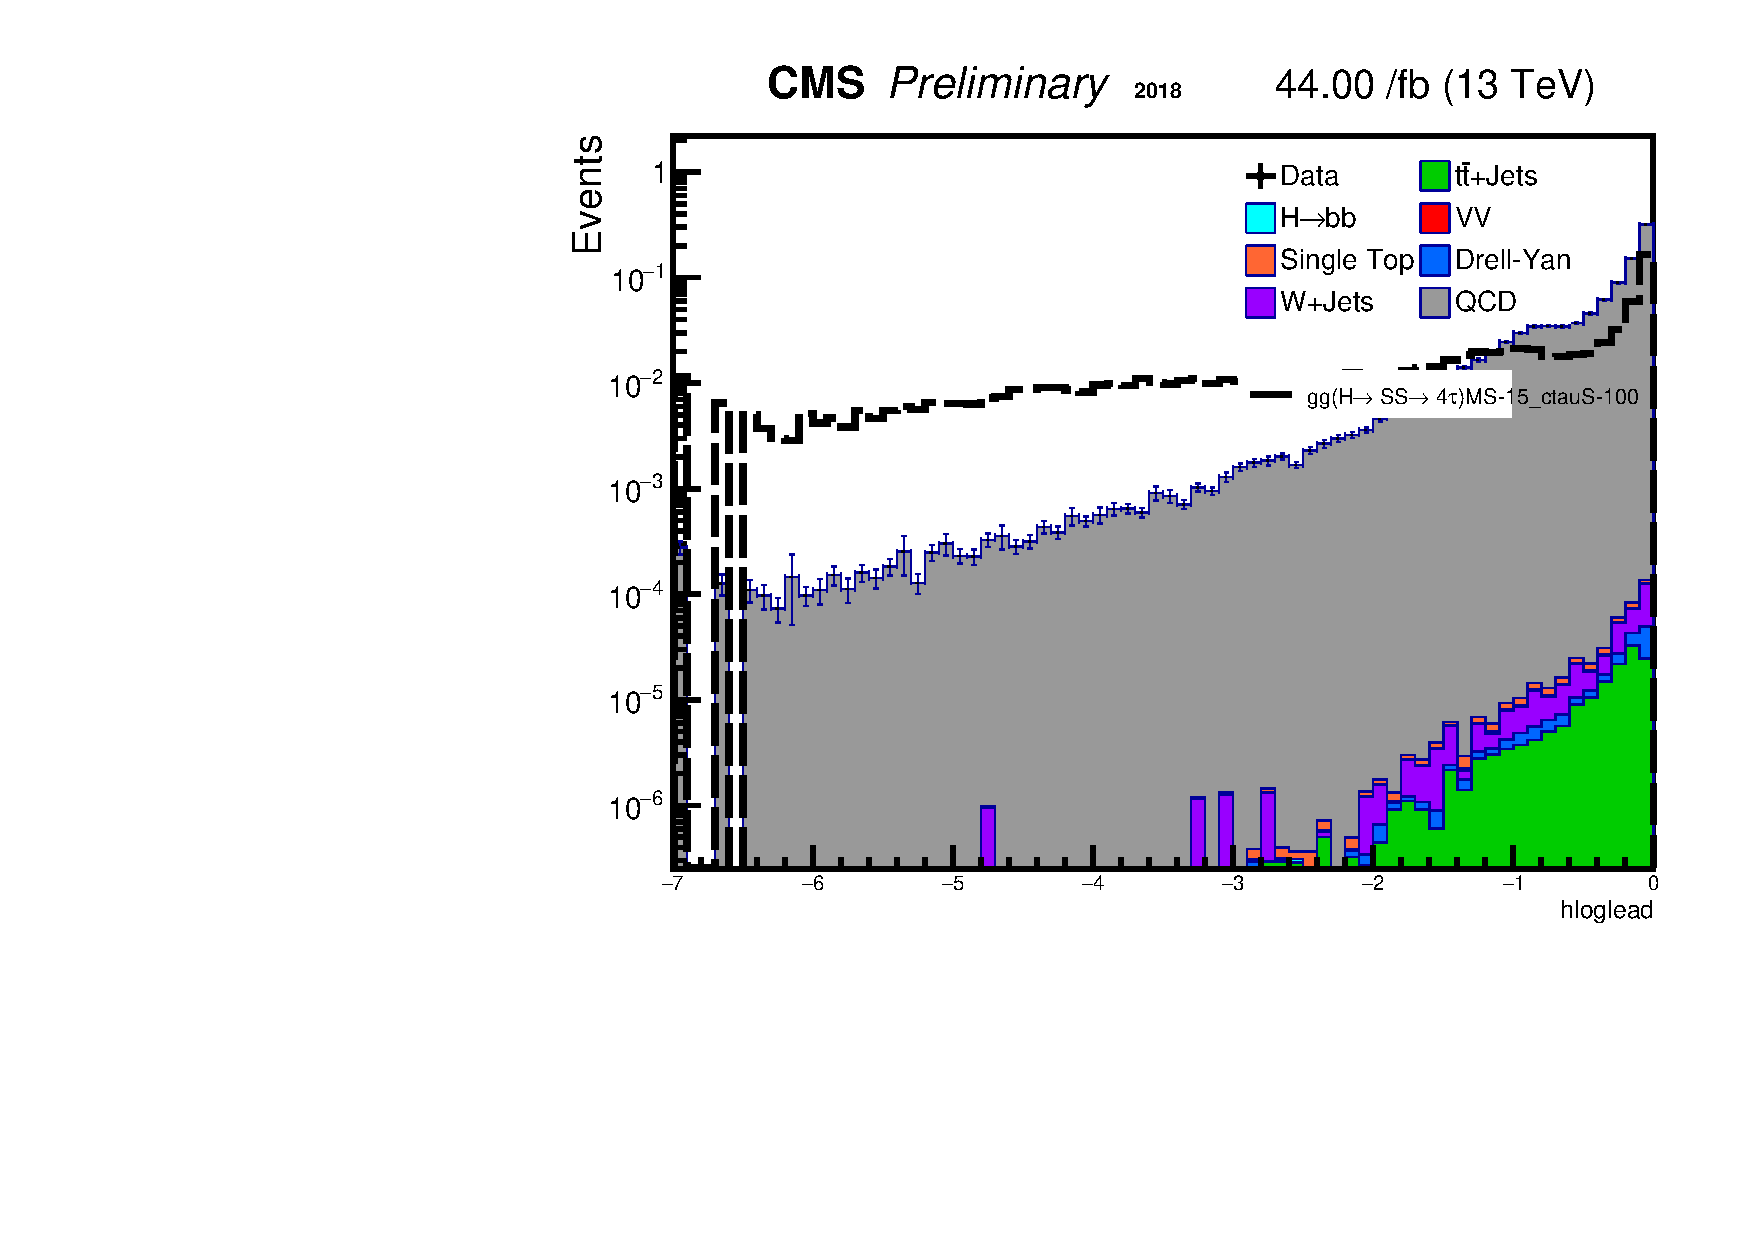
\includegraphics[width=0.47\linewidth]{figs/log_Oct6ANVars_MS-15_ctauS-100_hloglead.pdf}
   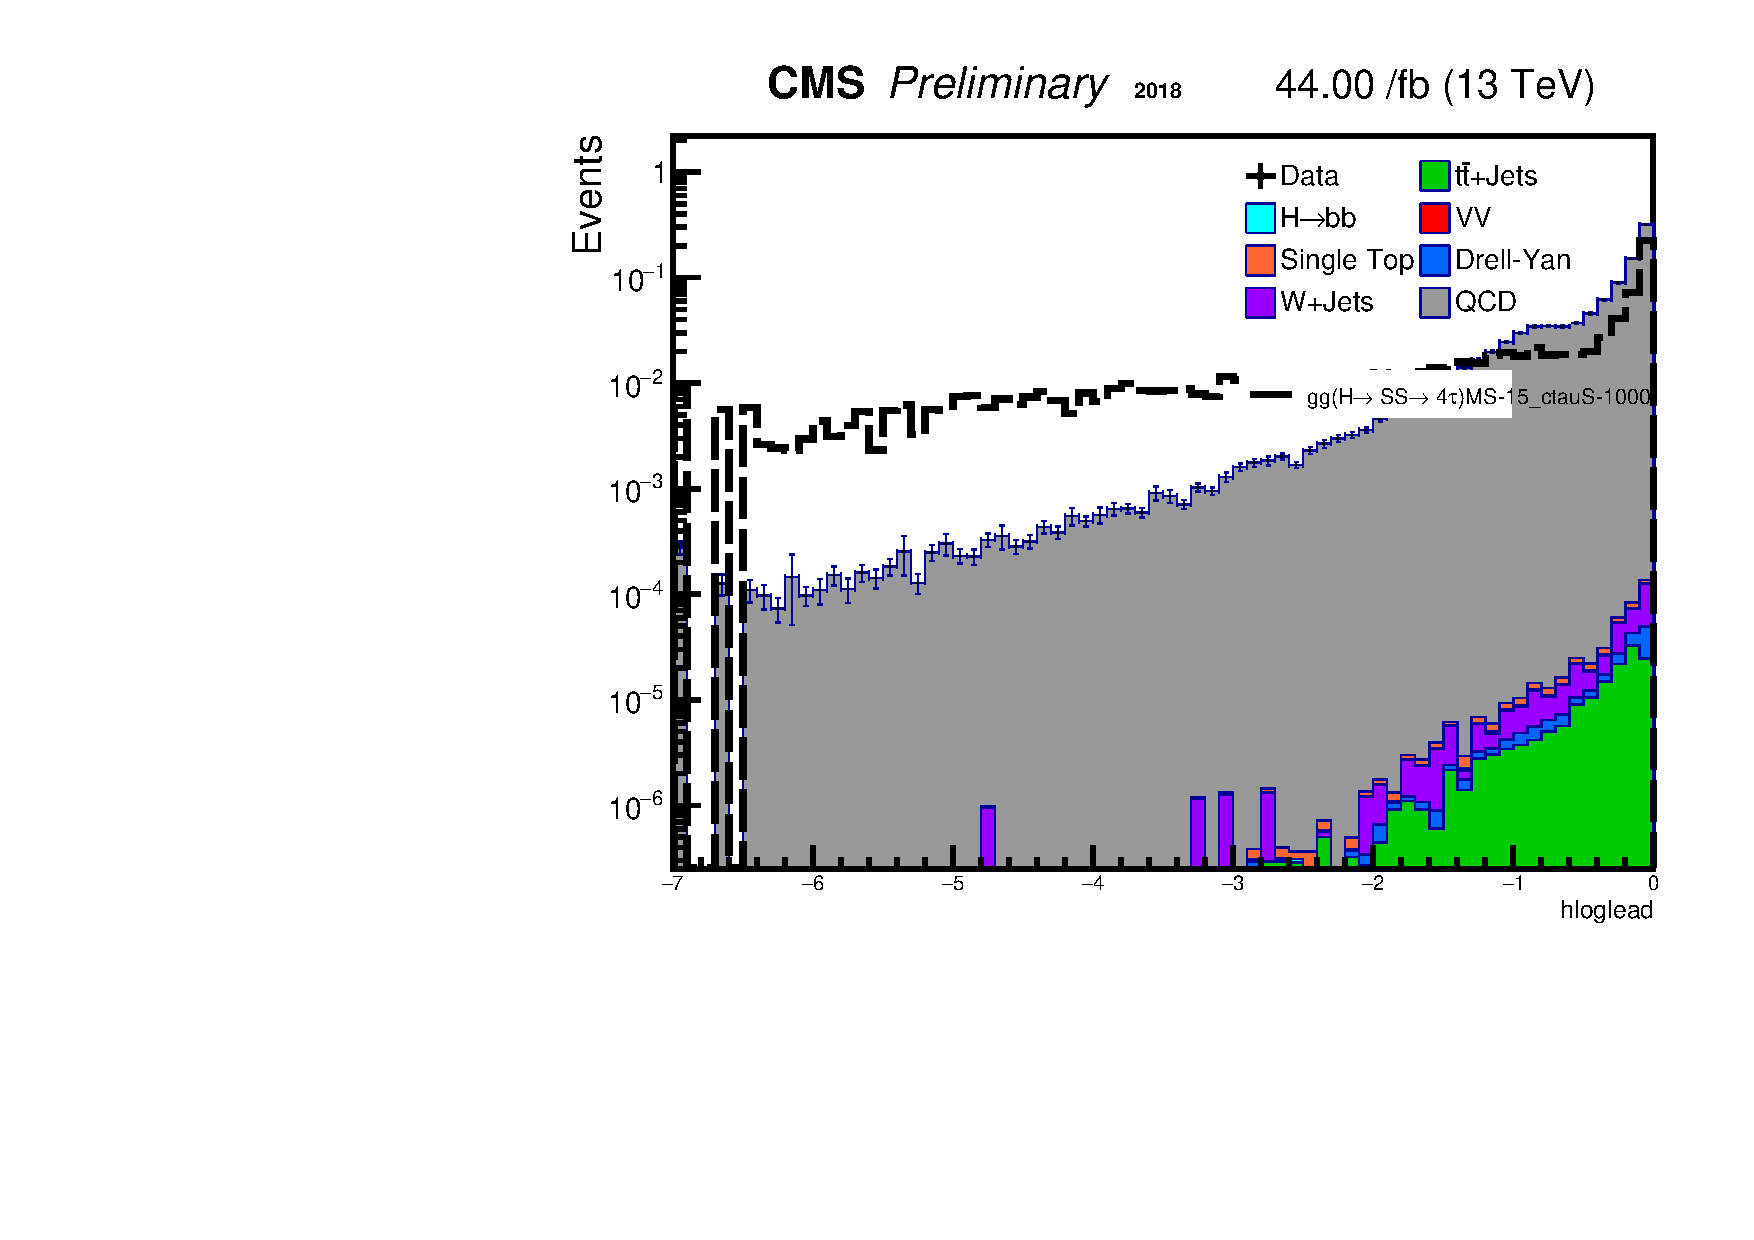
\includegraphics[width=0.47\linewidth]{figs/log_Oct6ANVars_MS-15_ctauS-1000_hloglead.pdf}
   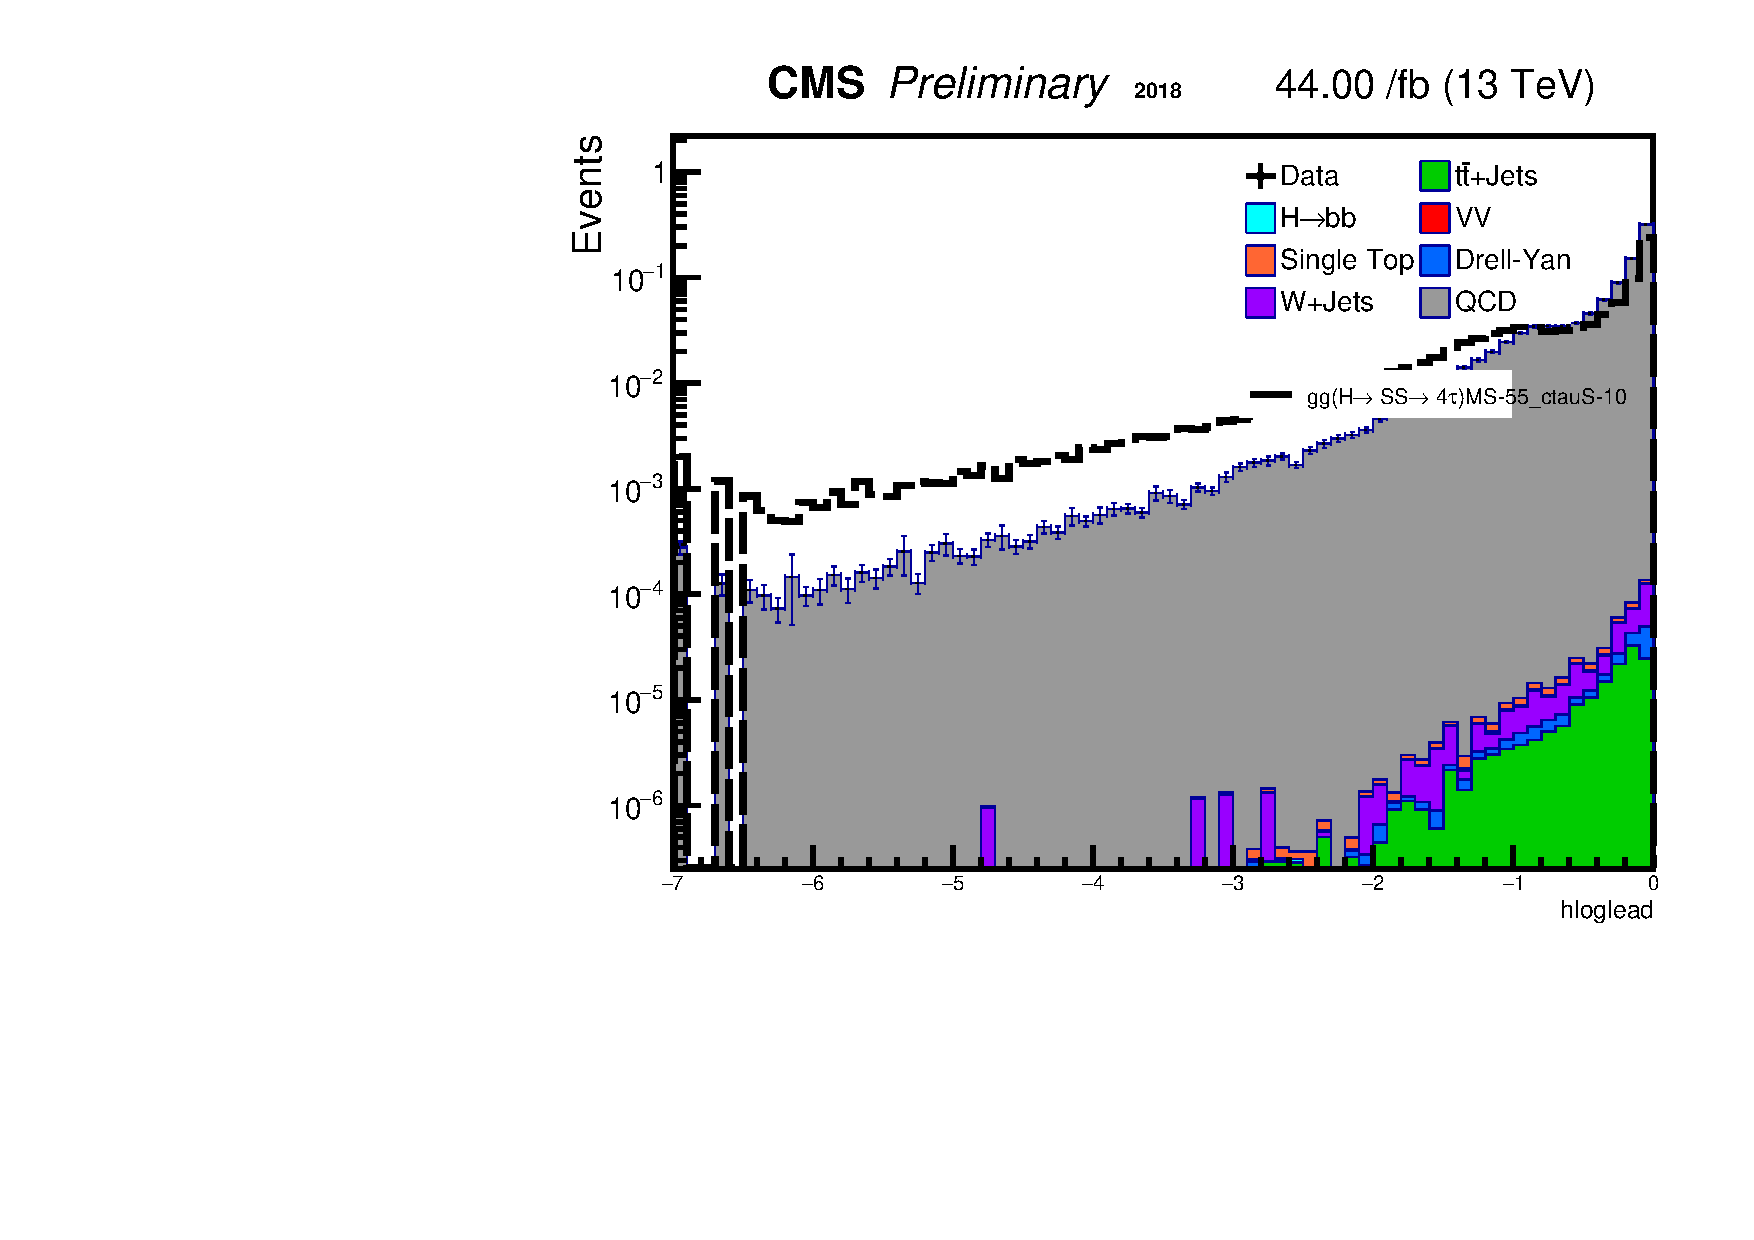
\includegraphics[width=0.47\linewidth]{figs/log_Oct6ANVars_MS-55_ctauS-10_hloglead.pdf}
   \caption{Signal versus Background for loglead, where the ROI score is the highest ROI of the event. Left plot is for MS-15\_ctauS-10mm point, whereas the right plot is for MS-15\_cauS-100mm point}
 \end{figure}


 \begin{figure}[h!]
   \label{fig:excROIscore}
   \centering
   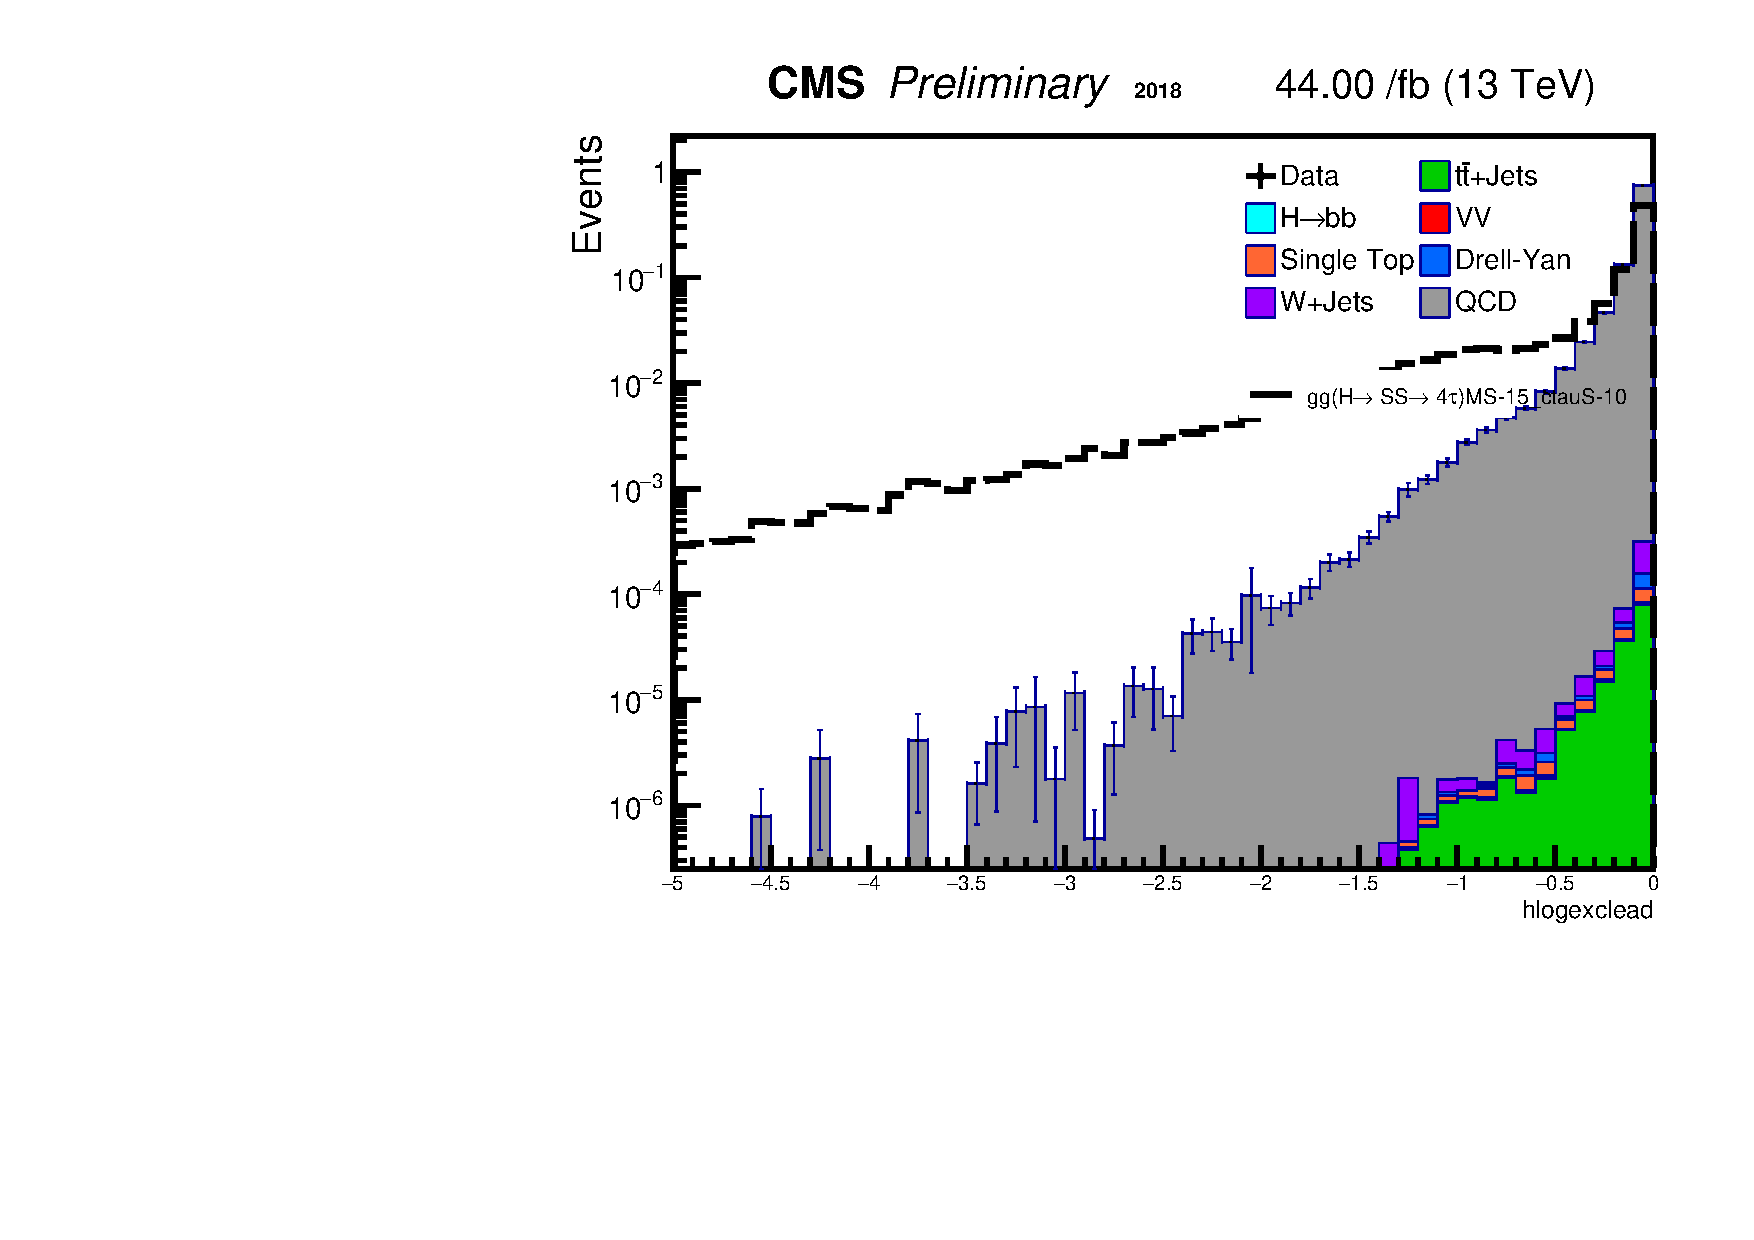
\includegraphics[width=0.47\linewidth]{figs/log_Oct6ANVars_MS-15_ctauS-10_hlogexclead.pdf}
   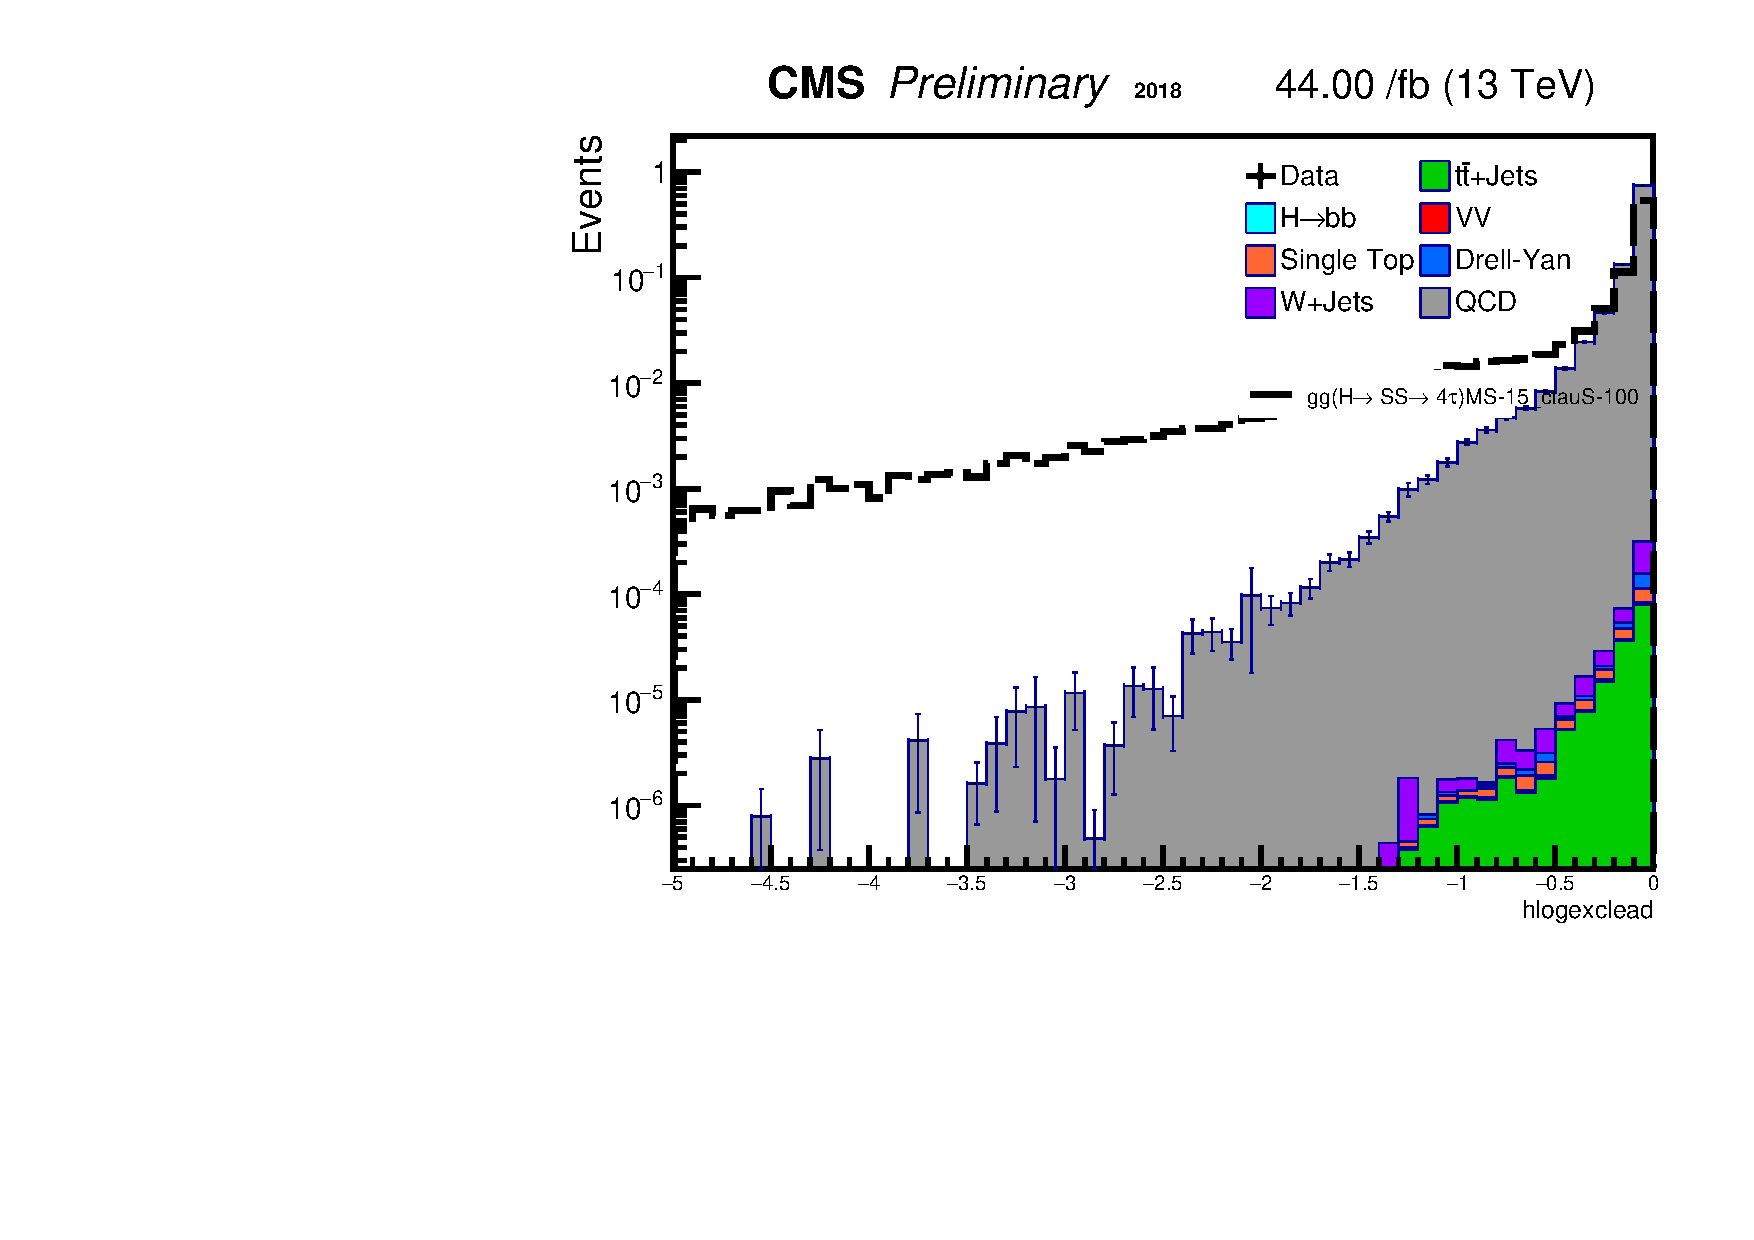
\includegraphics[width=0.47\linewidth]{figs/log_Oct6ANVars_MS-15_ctauS-100_hlogexclead.pdf}
   \includegraphics[width=0.47\linewidth]{figs/log_Oct6ANVars_MS-15_ctauS-1000_hlogexclead.pdf}
   \includegraphics[width=0.47\linewidth]{figs/log_Oct6ANVars_MS-55_ctauS-10_hlogexclead.pdf}
	 \caption{Signal versus Background for logexclead (sublead), where the ROI score is the second highest ROI (outside of dPhi=0.4 from leading ROI) of the event. Left plot is for MS-15\_ctauS-10mm point, whereas the right plot is for MS-15\_cauS-100mm point}
 \end{figure}

\begin{figure}[h!]
  \label{fig:DataMCscore}
  \centering
  \includegraphics[width=0.67\linewidth]{figs/Data_log_Oct6ANVars_MS-15_ctauS-10_hloglead.pdf}
  \includegraphics[width=0.67\linewidth]{figs/Data_log_Oct6ANVars_MS-15_ctauS-10_hlogexclead.pdf}
  \caption{Data/MC agreement for loglead and logexclead scores}
\end{figure}

\begin{figure}[h!]
  \label{fig:DataMCscore2}
  \centering
  \includegraphics[width=0.57\linewidth]{figs/Data_log_Oct6ANVars_MS-15_ctauS-10_hleaddxy.pdf}
  \includegraphics[width=0.57\linewidth]{figs/Data_log_Oct6ANVars_MS-15_ctauS-10_hexcleaddxy.pdf}
  \caption{Data/MC agreement for leading and subleading ROI distributions}

\end{figure}


\begin{figure}[h!]
  \label{fig:DataMCscore3}
  \centering
  \includegraphics[width=0.57\linewidth]{figs/Data_log_Oct6ANVars_MS-15_ctauS-10_leadROINumVert.pdf}
  \includegraphics[width=0.57\linewidth]{figs/Data_log_Oct6ANVars_MS-15_ctauS-10_excleadROINumVert.pdf}
  \caption{Data/MC agreement for leading and subleading ROI distributions}
\end{figure}


\begin{figure}[h!]
  \label{fig:DataMCscore4}
  \centering
  \includegraphics[width=0.57\linewidth]{figs/Data_log_Oct6ANVars_MS-15_ctauS-10_leadROIATNumber.pdf}
  \includegraphics[width=0.57\linewidth]{figs/Data_log_Oct6ANVars_MS-15_ctauS-10_excROIATNumber.pdf}
  \caption{Data/MC agreement for leading and subleading ROI distributions}

\end{figure}


\clearpage

\clearpage
\chapter{Event Selection, Signal and Control Regions}\label{sec:selections}
We have introduced the leading ROI's vertex score and subleading ROI's vertex score, which were both highly discirminant (Score ordering is based upon the vertex score).
Although we might have successful event selection with just triggers, and ROI vertex scores, we could strengthen the discriminant power further if we consider objects other than the trigger and ROIs(tracks).
These variables could be
\begin{itemize}
 \item Non-relevant to ROIs (muon, jet object)
 \item Missing input variable in the ROI training
\end{itemize}
These are not inputs of ML training, something that can't be learned by the ML, so not discriminated with scoring of the ROIs.
For this phenomenological situation, the analysis implements further event selection categories itemized below.
\begin{itemize}
  \item $\Delta\Phi(lead ROI,sublead ROI)$ 
  \item $\Delta R(lead ROI, Jet)<$0.6 
  \item 1 Isolated $\mu$
  \item Leading $\mu$'s transverse impact parameter significance to PV
\end{itemize}

Each of the cuts for the items above is motivated and explained in following subsections.

\section{Delta Phi(lead ROI,sublead ROI)}\label{sec:DeltaPhi}
This analysis looks for displaced vertices in the tracker region, coming from the decays of exotic LLPs from Higgs produced in gluon fusion mode, leaving the SM Higgs boson without boost.
The largest mass of the exotic LLPs is 55 GeV, ranging down to 7 GeV. 
Thus, exotic LLPs decayed from the SM Higgs become boosted, with their momentum vectors pointing back-to-back in the SM Higgs rest frame. 
Exotic LLPs with lighter mass are more boosted than heavier LLPs, since less LLP mass means more leftover energy into kinetic energy.
Given that ROIs corresponding to an exotic LLP's decay should have the highest ROI score, one should expect that the leading ROI and subleading ROI in a single event would be back-to-back.
Thus, in signal events, $\Delta\Phi$(lead ROI,sublead ROI) tends to have high values, while the background processes tend to have a more uniform distribution.
This analysis applies a cut above 2.2 to reduce background contribution. 
%Figure ~\ref{fig:dPhileadsub} shows the difference between the distribution of signal process and SM QCD backgrounds.


 \begin{figure}[h!]
   \caption{Signal versus Background for Delta Phi(leadROI, subleadROI). Left plot is for MS-15\_ctauS-10mm point, whereas the right plot is for MS-15\_cauS-100mm point}
   \label{fig:leadexcPosPhi}
   \centering
   \includegraphics[width=0.47\linewidth]{figs/AnalysisNoteplot_MS-15_ctauS-10_leadexcPosPhi.pdf}
   \includegraphics[width=0.47\linewidth]{figs/AnalysisNoteplot_MS-15_ctauS-100_leadexcPosPhi.pdf}
 \end{figure}

\section{Isolation criteria for muons}\label{ref:muISO}
As discussed in ~\ref{sec:triggers}, the main background for our analysis comes from QCD background events, especially from B-meson decay of QCD events with high ROI scores. 
Leptonic decay of B-meson generates muons, which trigger the B-parking trigger of the analysis.
Muons of B-meson decay have very poor isolation quality, just like ROIs formed around the B-meson decay.
In contrast, muons of $\tau$ lepton decay have better isolation quality.
In order to eliminate the dominant B-meson background from the QCD process, the analysis applies a PFISOLoose in selecting muon objects.
The precise definition of PFISOLoose is defined as below.
\begin{itemize}
  \item $(\Sigma pT(ch.had from PV)+max(0,\Sigma ET(neut.had) \Sigma ET (phot)-0.5* \Sigma pT(ch.had from PU)))/P_{T}(\mu)<0.25$
\end{itemize}

%Not only muons decayed from $\tau$ leptons with 55, 40GeV mass have a good isolation quality, but also muons of $\tau$ leptons from 15 GeV have a decent isolation quality based on gen-level $\Delta R(\tau,\bar_{\tau})$.
Some muons decayed from $\tau$ lepton with 7 GeV mass fail isolation cut, due to its poorer isolation quality from the boost.
However, it still benefits to apply the PFISOLoose cut on muons given it removes more background events than signal events.
The table below demonstrates event yield drop before and after requiring PFISOLoose cut on muons, classified by its signal and background process. 

\begin{tiny}
    \begin{table}
  \centering
\begin{tabular}{|p{3cm}|p{2cm}|p{2cm}|}
\hline
MC sample & events with BPH+1$\mu$ (noISO) & events with BPH+1$\mu$ (ISO) \\
\hline
 15to20 & 1 & 0.545 \\
 \hline
 20to30 & 1 & 0.407 \\
\hline
 30to50 & 1 & 0.295 \\
\hline
 50to80 & 1 & 0.144 \\
\hline
 80to120 & 1 & 0.078 \\
\hline
120to170 & 1 & 0.049 \\
\hline
170to300 & 1 & 0.032 \\
\hline
\textcolor{red}{ggH4$\tau$-MS7}& 1 & 0.619 \\
\hline
\textcolor{red}{ggH4$\tau$-MS15} & 1 & 0.855 \\
\hline
\textcolor{red}{ggH4$\tau$-MS40} & 1 & 0.910 \\
 \hline
    \end{tabular}
    \caption{Ptbinned Isocut}
    \end{table}
\end{tiny}    


\section{Leading muon's transverse impact parameter significance to PV}\label{ref:muIP}
With the B-Parking trigger, triggering muons have significant transverse displacement (impact parameter) in both background and signal processes.
However, displacement in the signal process is greater than the that of the background process.
The signal process has at minimum of c$\tau$ = 1mm, which is longer than B-meson lifetime.
Thus, triggering muon object's transverse impact parameter to PV is larger in signal process than background process.
In order to account for the error values associated with the parameter, we use impact parameter significance defined as the ratio of impact parameter divided by its error.
In order to adjust the orders of magnitude observed for the variable impact parameter significance (IPSig), we exploint log value of the IPSig.
The analysis implements a cut on this variable.


 \begin{figure}[h!]
   \caption{leading muon's transverse impact parameter value to the primary vertex. Left plot is for MS-15\_ctauS-10mm point, whereas the right plot is for MS-15\_cauS-100mm point}
   \label{fig:leadmuIP}
   \centering
   \includegraphics[width=0.47\linewidth]{figs/AnalysisNoteplot_MS-15_ctauS-10_leadmuIP.pdf}
   \includegraphics[width=0.47\linewidth]{figs/AnalysisNoteplot_MS-15_ctauS-100_leadmuIP.pdf}
 \end{figure}


\section{DeltaR(ROI, jet)}\label{ref:jetdR}
$\tau$ leptons of the signal process can also decay hadronically, while only one of the $\tau$ leptons decay muonically to trigger B parking trigger.
When $\tau$ leptons decay hadronically, its decay shower can get clustered in the calorimeter, and reconstructed as a jet.
Given the $\tau$ lepton's on-shell mass is a fixed value, $\tau$ lepton and its hadronic decay products (to-be clustered into a jet) have a specific kinematic phase space.
Thus, the $\Delta$ R(ROI, jet) has a distribution with a peak at a certain value (around 0.3-0.6).
Meanwhile, the QCD backround has a different distribution shape.
Given the hadronic nature of the process, jet multiplicity is high. 
Higher jet multiplicity makes the $\Delta$ R(ROI,jet) value to have a rather randomized value, resulting in a flat distribution. 

 \begin{figure}[h!]
   \caption{Delta R(Jet, leadingROI). Left plot is for MS-15\_ctauS-10mm point, whereas the right plot is for MS-15\_cauS-100mm point}
   \label{fig:ANleadSize}
   \centering
   \includegraphics[width=0.47\linewidth]{figs/AnalysisNoteplot_MS-15_ctauS-10_leadclosejetdR.pdf}
   \includegraphics[width=0.47\linewidth]{figs/AnalysisNoteplot_MS-15_ctauS-100_leadclosejetdR.pdf}
 \end{figure}


\section{Number of Annulus Tracks Associated with ROI}
 The tensorflow used for this analysis is trained with $p_T, \eta, \chi^{2}$, and other information of the annulus tracks (tracks that are inside ROI radius, but not fitted to vertex).
Meanwhile, an ROI's total number of annulus tracks is not a direct input for ML and tensorflow can only learn such information indirectly via annulus tracks' $p_T$.
Although having selected ROIs with high scores ($>$0.999), signal processes ROIs' number of annulus tracks show a quite different distribution from the background process.
%Figure ~\ref{fig:ANnum}
signal's high-scoring ROIs are mostly from the the exotic LLP scalar's decay into $\tau$ leptons. 
%The $\tau$ leptons have most 3 charged tracks for 12\%, and 1 charged track for 80\% of its decay mode ~\cite{willbedonelater}
Since the signal's high-score ROIs' are very well isolated, the ROI's number of annulus tracks is very low.
QCD background events, which are our dominant background, have a poor isolation quality.
Since QCD's high-scoring ROI's are poorly isolated due to QCD nature, these ROIs' numbers of annulus tracks are higher than the signal.
More precisely, QCD's high-scoring ROI's are usually from B-mesons, which have higher track multiplicity than $\tau$ leptons.


%% \begin{figure}[h!]
 \begin{figure}[h!]
   \caption{Number of tracks in the annulus cone of the leading ROI. Left plot is for MS-15\_ctauS-10mm point, whereas the right plot is for MS-15\_cauS-100mm point}
   \label{fig:ANleadSize}
   \centering
   \includegraphics[width=0.47\linewidth]{figs/AnalysisNoteplot_MS-15_ctauS-10_leadROIATNumber.pdf}
   \includegraphics[width=0.47\linewidth]{figs/AnalysisNoteplot_MS-15_ctauS-100_leadROIATNumber.pdf}
 \end{figure}


%\section{Number of Annulus Tracks Associated with ROI}\label{ref:NumAnnulus}
% The tensorflow used for this analysis is trained with $p_T, \eta, \chi^{2}$, and other information of the annulus tracks (tracks that are inside ROI radius, but not fitted to vertex).
%Meanwhile, an ROI's total number of annulus tracks is not a direct input for ML and tensorflow can only learn such information indirectly via annulus tracks' $p_T$.
%Although having selected ROIs with high scores ($>$0.999), signal processes ROIs' number of annulus tracks show a quite different distribution from the background process.
%%Figure ~\ref{fig:ANnum}
%signal's high-scoring ROIs are mostly from the the exotic LLP scalar's decay into $\tau$ leptons. 
%%The $\tau$ leptons have most 3 charged tracks for 12\%, and 1 charged track for 80\% of its decay mode ~\cite{willbedonelater}
%Since the signal's high-score ROIs' are very well isolated, the ROI's number of annulus tracks is very low.
%QCD background events, which are our dominant background, have a poor isolation quality.
%Since QCD's high-scoring ROI's are poorly isolated due to QCD nature, these ROIs' numbers of annulus tracks are higher than the signal.
%More precisely, QCD's high-scoring ROI's are usually from B-mesons, which have higher track multiplicity than $\tau$ leptons.
%
%
%%% \begin{figure}[h!]
% \begin{figure}[h!]
%   \caption{Number of tracks in the annulus cone of the leading ROI. Left plot is for MS-15\_ctauS-10mm point, whereas the right plot is for MS-15\_cauS-100mm point}
%   \label{fig:ANleadSize}
%   \centering
%   \includegraphics[width=0.47\linewidth]{figs/AnalysisNoteplot_MS-15_ctauS-10_leadROIATNumber.pdf}
%   \includegraphics[width=0.47\linewidth]{figs/AnalysisNoteplot_MS-15_ctauS-100_leadROIATNumber.pdf}
% \end{figure}
%
%
%

\clearpage

\clearpage
\chapter{Background Estimation}\label{sec:estimate}

\begin{figure}[h!]
	\caption{Data/MC agreement for distributions. High ROI scores and high Log10(muIPSig) values lack MC statistics}
  \label{fig:DataMCscore5}
  \centering
  \includegraphics[width=0.40\linewidth]{figs/Data_log_AnalysisNote_MS-15_ctauS-10_hlogexclead.pdf}
  \includegraphics[width=0.40\linewidth]{figs/Data_log_AnalysisNote_MS-15_ctauS-10_AmpLog10muIPSig.pdf}

\end{figure}
Section ~\ref{sec:selections} listed several different discriminant variables for the analysis.
Leading ROI vertex score, subleading ROI vertex score, and leading muon's IP value have the most discriminatory power.
Although the background MC samples describe the data's distribution reasonably well, one can also see discrepancies at higher vertex scores and IPSig values.
The discrepancy originates from 2 different reasons.
First, the lack of statistics is a fundamental deficiency for the MC samples.
Unlike 11.9 billion b-parking data events, MC sample events are simulated with extremely intensive computing resources.
Thus, its event number is below 100 million at most, failing to describe distributions for extreme values.
Second, the QCD MC's data description accuracy is lacking compared to other physics processes.
QCD background, the main background for the analysis, is a quantum-chromodynamics process.
QCD involves much uncertainty and relies on probabilistic description at low energy.
Therefore, QCD's description accuracy is lacking compared to other processes, such as WJets and the Drell-Yan process.
Since MC does not adequately describe the data, the analysis uses data-driven background estimation method.




\section{ABCD method}
ABCD method is the most preferred for any background estimation method thanks to its simplicity.
ABCD method is the simplest form of transfer factor.
A ratio of background events at two control regions (CR) is applied to another CR's background event to infer background events in signal regions (SR) without unblinding.
The simplest mathematical for is described in formula \ref{eq:ABCD}.
\begin{equation}
\label{eq:ABCD}
	SR:CR1=CR2:CR3, SR=CR1*\frac{CR2}{CR3} 
\end{equation}

ABCD method requires two variables used for its estimation to be independent of each other for the background process.


Unfortunately, leading ROI and subleading ROI vertex scores are correlated in the QCD background process.
ROIs from B-mesons score higher in our TensorFlow.
In QCD processes, the B-mesons are likely to be pair produced.
Therefore, when the leading ROI vertex score is high due to a B-meson, the subleading ROI vertex score is also high because the other meson is produced at the same time.
Thus, due to their correlation, leading and subleading scores cannot be our ABCD discriminant variable candidates.

The analysis selects leading ROI and leading muon's IP value as its ABCD discriminant variables.
After implementing all other cuts (sublead ROI, $\Delta\Phi(lead,sublead)$, Annulus score, 1 Isolated $\mu$, $\Delta R(lead ROI, Jet)$), we tested the correlation factor between the leading ROI, and leading mu's IPSig values for each background process.
The values are pretty minimal except for 2-3 processes where there were too few entries to derive a solid conclusion due to statistical limitations.
%Therefore, the analysis uses leading Log10(IPSig) and leading ROI vertex score for its ABCD discriminant variables.
 \begin{figure}[h!]
   \caption{Cutflow histogram of Signal versus background. The signal is MS15GeV-ct10mm point. Last bin of the cutflow histogram is ABCD region selection. Top left plot is for region A, whereas the bottom right plot is for region D}
   \label{fig:ABmethod}
   \centering
   \includegraphics[width=0.47\linewidth]{figs/log_CutflAnalysisNote_MS-15_ctauS-10_A_Cutflow.pdf}
   \includegraphics[width=0.47\linewidth]{figs/log_CutflAnalysisNote_MS-15_ctauS-10_B_Cutflow.pdf}
   \includegraphics[width=0.47\linewidth]{figs/log_CutflAnalysisNote_MS-15_ctauS-10_C_Cutflow.pdf}
   \includegraphics[width=0.47\linewidth]{figs/log_CutflAnalysisNote_MS-15_ctauS-10_D_Cutflow.pdf}
 \end{figure}

% \begin{figure}[h!]
%   \caption{Cutflow histogram of MS55GeV-ct10mm point. Left plot is for region A, whereas the right plot is for region D}
%   \label{fig:ABmethod2}
%   \centering
%   \includegraphics[width=0.47\linewidth]{figs/log_CutflAnalysisNote_MS-55_ctauS-10_A_Cutflow.pdf}
%   \includegraphics[width=0.47\linewidth]{figs/log_CutflAnalysisNote_MS-55_ctauS-10_B_Cutflow.pdf}
%   \includegraphics[width=0.47\linewidth]{figs/log_CutflAnalysisNote_MS-55_ctauS-10_C_Cutflow.pdf}
%   \includegraphics[width=0.47\linewidth]{figs/log_CutflAnalysisNote_MS-55_ctauS-10_D_Cutflow.pdf}
% \end{figure}
 \begin{figure}[h!]
   \caption{Final bin of cutflow}
   \label{fig:Finalbin}
   \centering
   \includegraphics[width=0.67\linewidth]{figs/log_CutflAnalysisNote_MS-15_ctauS-10_ABCD_final_rate.pdf}
 \end{figure}

\section{Validation of ABCD method}
Although background MC's correlation factor($\hat{r}$) values are small, we need to verify that the data's correlation factor is negligible since data will be used for our background estimation.
However, direct computation of $\hat{r}$(leadROI,Log10(muIPSig)) for data is problematic because CMS collaboration stipulates ``blinding.''
In general, a high signal ratio is expected in the signal region.
In order to avoid bias for discovery and to change their analysis strategy accordingly, CMS collaboration recommends physicists blind themselves from looking into data entry in the signal region until community acknowledgment is granted.
This concept is called ``blinding.''
Since one can not access data entry in the signal region, the data's correlation factor($\hat{r}$) can not be computed.
Therefore, one needs to find an alternative way to estimate data's $\hat{r}$(leadROI,Log10(muIPSig)) without unblinding data in the signal region.

For this purpose, we define a new ABCD region, referred to as A'B'C'D'.
A'-D' region is an orthogonal plane to the original ABCD, where the $\Delta\Phi$(lead,exclead) category of the event selection is flipped while all other event selection cuts are removed.
Region A', a correspondent Signal region of the orthogonal plane, should be much lower in the signal ratio (background dominated): Only so, looking into data entry in A' is not problematic.
In figures a-b, we confirm that the background dominates the A' region while the signal is low regardless of the signal's MS and ctau.

\begin{figure}[h!]
  \caption{Cartoon description of ABCD method validation. The first figure shows a simpler definition of validation region. The second figure shows a more sophisiticated definition of validation regions. }
  \label{fig:valcar}
  \centering
  \includegraphics[width=0.85\linewidth]{figs/SimpleVR.png}
  \includegraphics[width=0.85\linewidth]{figs/SophiVR.png}

\end{figure}


\begin{figure}[h!]
  \caption{Profile plot of VR1}
  \label{fig:valcar2}
  \centering
  \includegraphics[width=0.65\linewidth]{figs/VR1.png}

\end{figure}

\begin{figure}[h!]
  \caption{Profile plot of VR2}
  \label{fig:valcar2}
  \centering
  \includegraphics[width=0.65\linewidth]{figs/VR2.png}

\end{figure}

\begin{figure}[h!]
  \caption{Profile plot of VR3}
  \label{fig:valcar3}
  \centering
  \includegraphics[width=0.65\linewidth]{figs/VR3.png}

\end{figure}
In A'-D' region, we can see the correlation factor is about 10\%, still a negligible value.


With $\hat{r}$(leadROI,Log10(muIPSig)) value in A'-D' region, It seems sufficient to claim that there should be a negligible correlation between leadROI and Log10(muIPSig) for the A-D region as well.
Unfortunately, suspicious people could throw one last question.
What if $\hat{r}$(leadROI,Log10(muIPSig)) value changes with respect to $\Delta\Phi$(lead,exclead)?
If the formula in \ref{eq:rhat} is not true, $\hat{r}$(leadROI,Log10(muIPSig)) obtained from A'-D' is not a good estimate for $\hat{r}$(leadROI,Log10(muIPSig)) for A-D.


\begin{equation}
\label{eq:rhat}
	\frac{d\hat{r}(leadROI,Log10(muIPSig))}{d\Delta\Phi(lead,exc)}=0
\end{equation}
We subdivide A'-D' to check that formula \ref{eq:rhat} is true.
A1'-D1' are orthogonal planes where $\Delta\Phi$(lead,exclead) is closest to A-D. 
Increasing numeric value indicates how far the $\Delta\Phi$(lead,exclead) is from the A-D. 
$\hat{r}$(leadROI,Log10(muIPSig)) value for each of A'-D' region is plotted in figures and summarized in table.



As we scan $\hat{r}$(leadROI,Log10(muIPSig)) for each $\Delta\Phi$(lead,exclead) section, very small trend with respect to $\Delta\Phi$(lead,exclead) is observed.
We can claim the formula \ref{eq:rhat} is true and $\hat{r}$(leadROI,Log10(muIPSig)) from A'-D' can be translated into A-D region as well.
Since there is little correlation between the two variables for the ABCD region, we validated the background estimation method.
With the background rate in the signal region estimated by the ABCD method with data, and with signal MC, we can either claim there exists a signal over the SM expectation or not.
If it does not, we can claim an exclusion limit on the branching ratio of the signal process to a specific value.

Before that final step, systematic uncertainty is described in the following section for exclusion limit calculation.


\clearpage

\clearpage
\chapter{Systematic Uncertainties}\label{sec:systs}
Table \ref{tab:systab} shows a summary of the systematic uncertainties included for the exclusion limit calculation,

\begin{table}[htb!]
  \caption{Systematic Uncertainty Table}
  \begin{center}
    \begin{tabular}{l|l|l}\hline
     Uncertainty    & Signal (\%) & Background (\%)\\
      \hline
     Luminosity     & 2 & 2\\
      \hline
     Muon ID,ISO Scale Factor     & 2 & 2 \\
      \hline
     ROI Score      & 10 & -\\
      \hline
     Background Estimation Method     & 20 & - \\
      \hline
     Statistical error     & 6 & 20 \\
      \hline
    \end{tabular}
    \label{tab:systab}
  \end{center}
\end{table}
CMS records the delivered luminosity, which is accompanied by its uncertainty.
This uncertainty is universal and applied to every analysis.
For data collected in 2018, the luminosity uncertainty is found to be 1.8\%, which is applied to both signal and background \cite{lumiUnc18}.
The analysis uses muon objects applied with Loose ID and ISO criteria.
Lepton ID, ISO scale factors, provided by the muon POG \cite{muonpog}, also carry uncertainty, albeit the magnitude is minimal.
The ROI score uncertainty is obtained by adjusting the leading ROI's vertex score.
As discussed in chapter \ref{sec:estimate}, we validated the ABCD method using a validation region of A'-D'.
The correlation factor of 2 variables in A'-D' was a small value of 11\%.
It tells us there could be an 11\% or slightly larger correlation in the A-D region.
A positive correlation implies more background concentrated in the SR(A) than its estimated rate(B*C/D), which would be about 11\%.
To be conservative with the estimation method, we set uncertainty sourced by the background estimation method at 20\%.
Last, our signal MC in SR(A) has enough statistics.
However, it is not infinite.
Therefore, we need to consider the statistical error of the signal MC in the signal region.
We have 300 events in signal region A, which results in 6\% of statistical error from $\frac{\sqrt{N}}{N}$, $\frac{30}{300}$.
Likely the background rate in the SR(A) is calculated with B*C/D.
Its propagated statistical uncertainty is 20\%

\clearpage

\clearpage
\chapter{Results}\label{sec:results}
Unblinded result data no excess over the standard model prediction.
Exclusion limit plot.
Results
 \begin{figure}[h!]
   \caption{Current Preliminary limit plots}
   \label{fig:Limit}
   \centering
   \includegraphics[width=0.48\linewidth]{figs/7GeVUpperLimit.pdf}
   \includegraphics[width=0.48\linewidth]{figs/15GeVUpperLimit.pdf}
 \end{figure}
 \begin{figure}[h!]
   \caption{Current Preliminary limit plots}
   \label{fig:Limit2}
   \centering
   \includegraphics[width=0.48\linewidth]{figs/40GeVUpperLimit.pdf}
   \includegraphics[width=0.48\linewidth]{figs/55GeVUpperLimit.pdf}
 \end{figure}

\clearpage

\clearpage
\chapter{Conclusions}\label{sec:conclusions}
This was an interesting analysis targeting tau lepton final state with tracker lifetime

\clearpage


\bibliography{auto_generated}

%%% DO NOT ADD \end{document}!
